%!TEX program = xelatex
%!TEX options=--shell-escape
\documentclass[12pt]{article}

%
\usepackage[scheme=plain]{ctex}
%
\usepackage{fontspec}
%
\usepackage[margin = 1in]{geometry}

%
\usepackage[dvipsnames]{xcolor}
\usepackage[many]{tcolorbox}

%
\usepackage{amsmath}
\usepackage{amssymb}
\usepackage{amsthm}
%
\usepackage{tensor}
%
\usepackage{slashed}
\usepackage{physics}
\usepackage{simpler-wick}

%
\usepackage[version=4]{mhchem}

%
\usepackage{mathtools}

%
\usepackage{bm}
\newcommand{\dbar}{\dif\hspace*{-0.18em}\bar{}\hspace*{0.2em}}
\DeclareMathAlphabet\mathbfcal{OMS}{cmsy}{b}{n}
%\usepackage{bbold}
\newcommand*{\dif}{\mathop{}\!\mathrm{d}}
\newcommand*{\euler}{\mathrm{e}}
\newcommand*{\imagi}{\mathrm{i}}

\renewcommand{\vec}[1]{\boldsymbol{\mathbf{#1}}}

\usepackage{caption}

\usepackage{enumitem}

\usepackage{multirow}
%
\usepackage{mathrsfs}
\usepackage{dsfont}

%
\usepackage{hyperref}
\hypersetup{
    colorlinks=true,
    linkcolor=violet,
    filecolor=blue,      
    urlcolor=blue,
    citecolor=cyan,
}

%
\usepackage{graphicx}
\usepackage{subfig}
\usepackage{subcaption}
%
\graphicspath{{figures/}}


%
\usepackage{indentfirst}
%
\setlength{\parindent}{2em}
\linespread{1.25}

% 
% \setmainfont{Times New Roman}

\title{Note}
\author{Feng-Yang Hsieh}
\date{}

\begin{document}
\maketitle

\section{Sample}% (fold)
\label{sec:sample}
	The vector boson samples are generated from \textsc{MadGraph5 aMC@NLO 3.3.1}. Then pass to Pythia for showering and hadronization. Then pass to Delphes for detector simulation. 	

	The processes are the VBF production for doubly charged Higgses $H_5^{\pm\pm}$ and heavy neutral Higgses $H_5$ with decays $H_5^{\pm\pm} \to W^{\pm}W^{\pm} \to jjjj$ and $H_5\to ZZ \to jjjj$.

	Following are the MadGraph scripts for generating $W^{+}$ sample:
	\begin{verbatim}
	import model GM_NLO
	define v = z w+ w-
	generate p p > H5pp j j $$v, (H5pp > w+ w+, (w+ > j j), (w+ > j j))
	output VBF_H5pp_ww_jjjj
	launch VBF_H5pp_ww_jjjj

	shower=Pythia8
	detector=Delphes
	analysis=OFF
	done

	set param_card tanth 0.226480
	set param_card lam2 0.070070
	set param_card lam3 -1.331328
	set param_card lam4 1.364671
	set param_card lam5 -1.963271
	set param_card M1coeff 1046.827111
	set param_card M2coeff 135.30791

	set run_card nevents 100000
	set run_card ebeam1 6500.0
	set run_card ebeam2 6500.0
	set run_card cut_decays True
	set run_card ptj 50
	set run_card etaj 3

	/home/r10222035/boosted_V_ML_test/Cards/delphes_card.dat

	done	
	\end{verbatim}

	In Delphes, jets are constructed by the anti-$k_t$ algorithm with $R = 0.7$.

	\subsection{Sample selection}% (fold)
	\label{sub:sample_selection}
		Only the events that satisfy the following requirement will use for training.
		\begin{enumerate}
			\item The transverse momentum of jets are required $p_\text{T} \in (350, 450) \text{ GeV}$ and in range $\abs{\eta}<1$.
			\item Merging: The angular distance between the two quarks decayed from the vector boson is required $\Delta R(q_1,q_2) < 0.6$.
			\item Matching: The vector boson and jet are matched if $\Delta R(V,j) < 0.1$. The events with less than two matching jets will be discarded.
		\end{enumerate}
	% subsection sample_selection (end)
	
	\subsection{Sample pre-processing}% (fold)
	\label{sub:sample_pre_processing}
		The jet charge of a jet is defined as
		\begin{equation}
			\mathcal{Q}_\kappa \equiv \frac{1}{(p_{\text{T}, J})^{\kappa}} \sum_{i\in J} q_i \times \left( p_{\text{T}}^{i} \right)^{\kappa}
		\end{equation}
		where $i$ represents the constituent in the jet $J$.

		\subsubsection{Jet image}% (fold)
		\label{subs:jet_image}
			After the sample selection, we can construct the jet image of the matching vector boson jet. The jet image is constructed by the following steps:
			\begin{enumerate}
				\item Centralization: Calculating the $p_\text{T}$ weighted center in $\eta,\phi$ plane, then shift this point to origin.
				\item Rotation
				\item Flipping
				\item Pixelating in $\Delta\eta = \Delta\phi = 1.6$ box, with $75\times 75$ pixels.
			\end{enumerate}
		% subsubsection jet_image (end)	
	% subsection sample_pre_processing (end)
	\subsection{Plots}% (fold)
	\label{sub:plots}
		Figure \ref{fig:jet_mass_distribution} is the jet mass distribution.
		\begin{figure}[htpb]
			\centering
			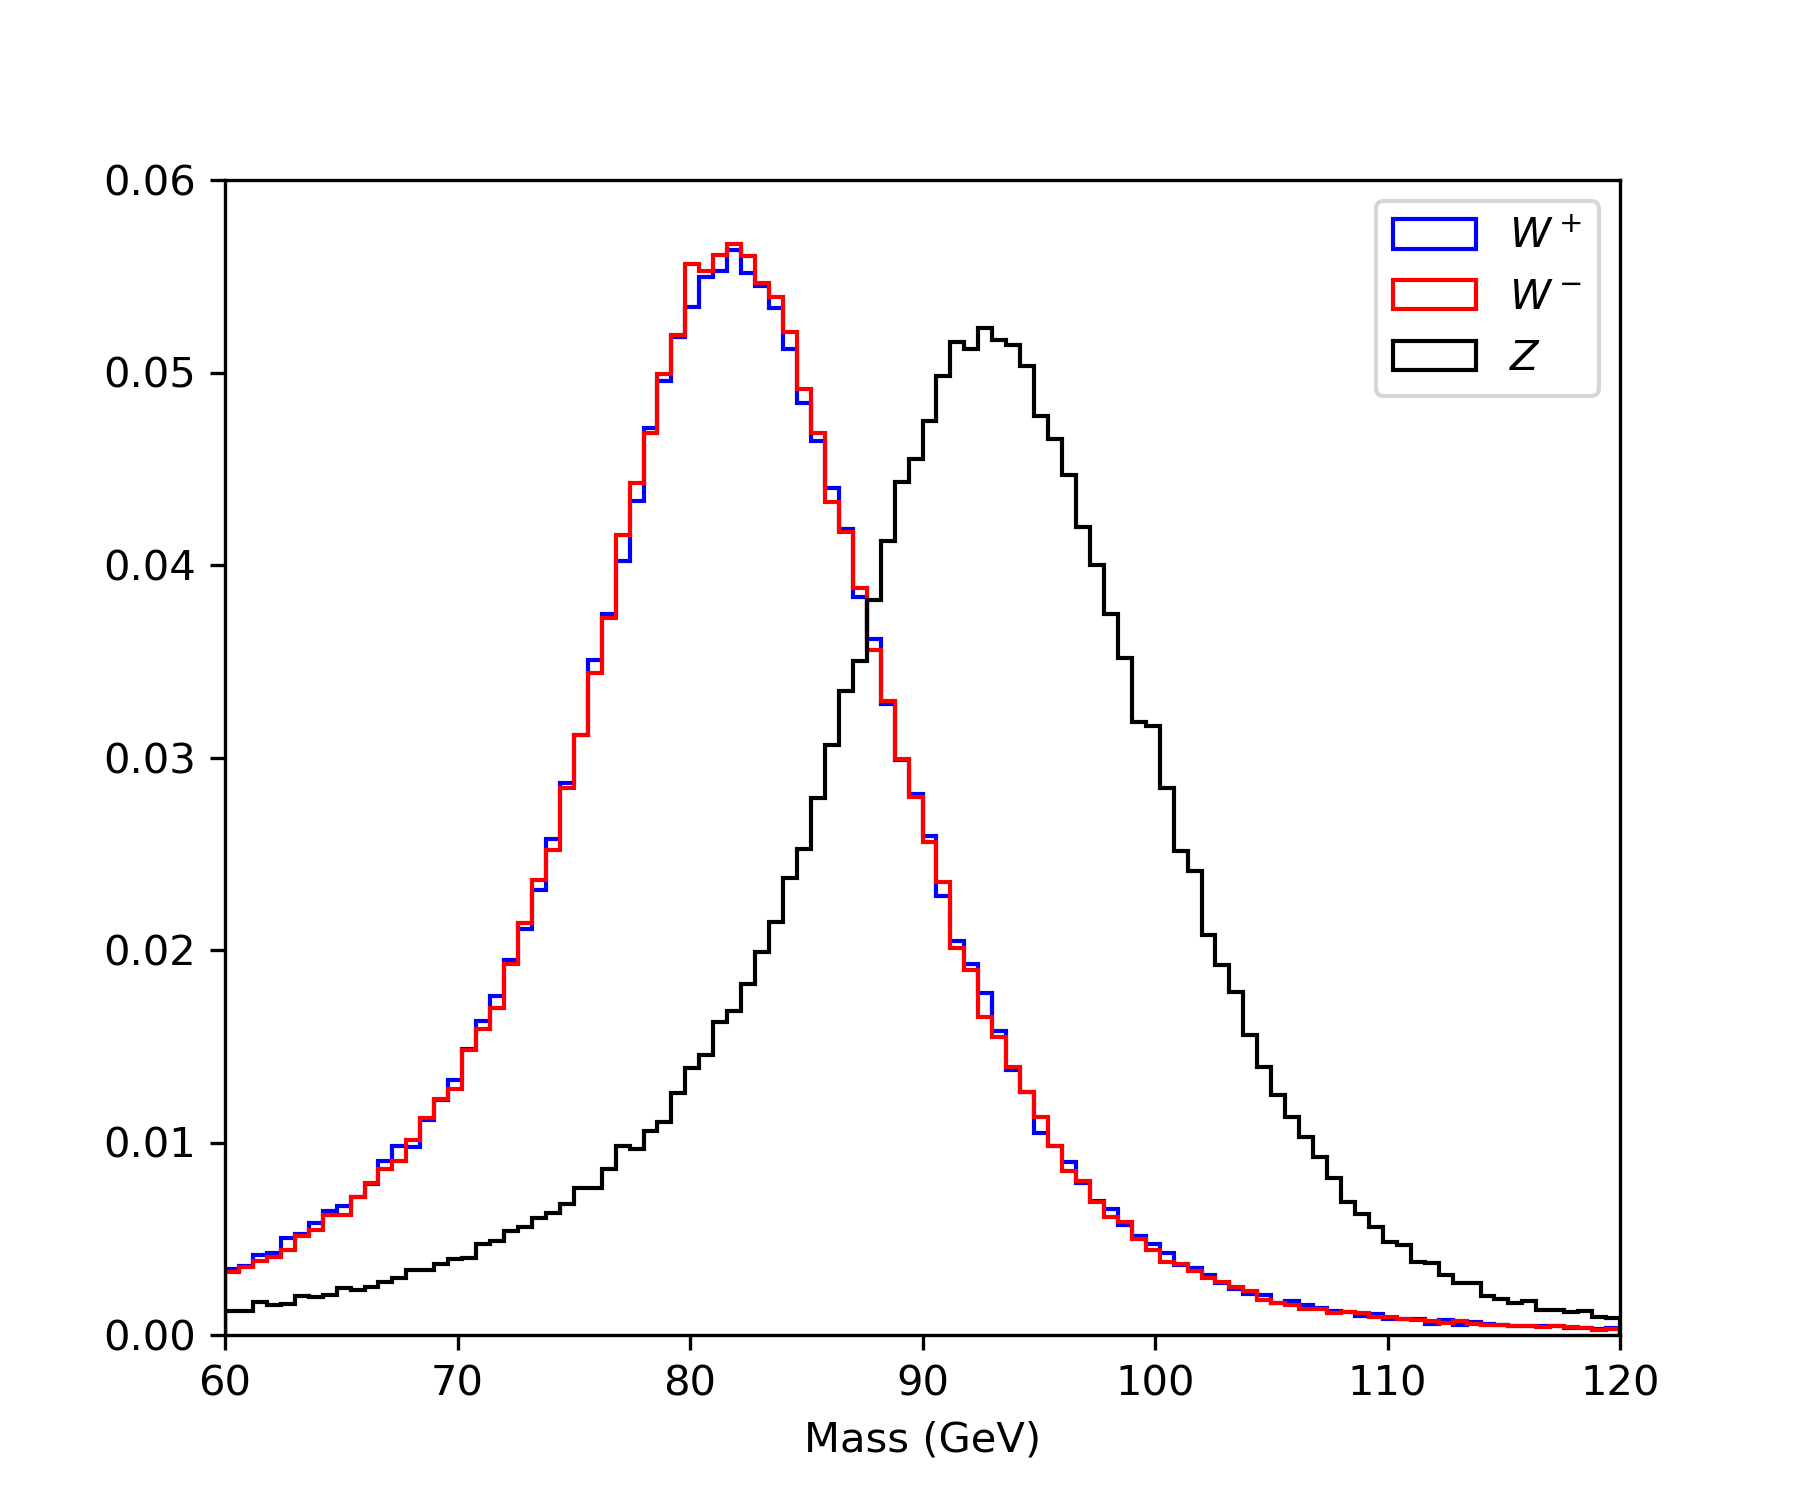
\includegraphics[width=0.5\textwidth]{jet_mass_distribution.png}
			\caption{Jet mass distributions of their vector boson samples.}
			\label{fig:jet_mass_distribution}
		\end{figure}

		Figure \ref{fig:jet_charge_different_kappa} is the jet charge distributions with different $\kappa$.
		\begin{figure}[htpb]
			\centering
			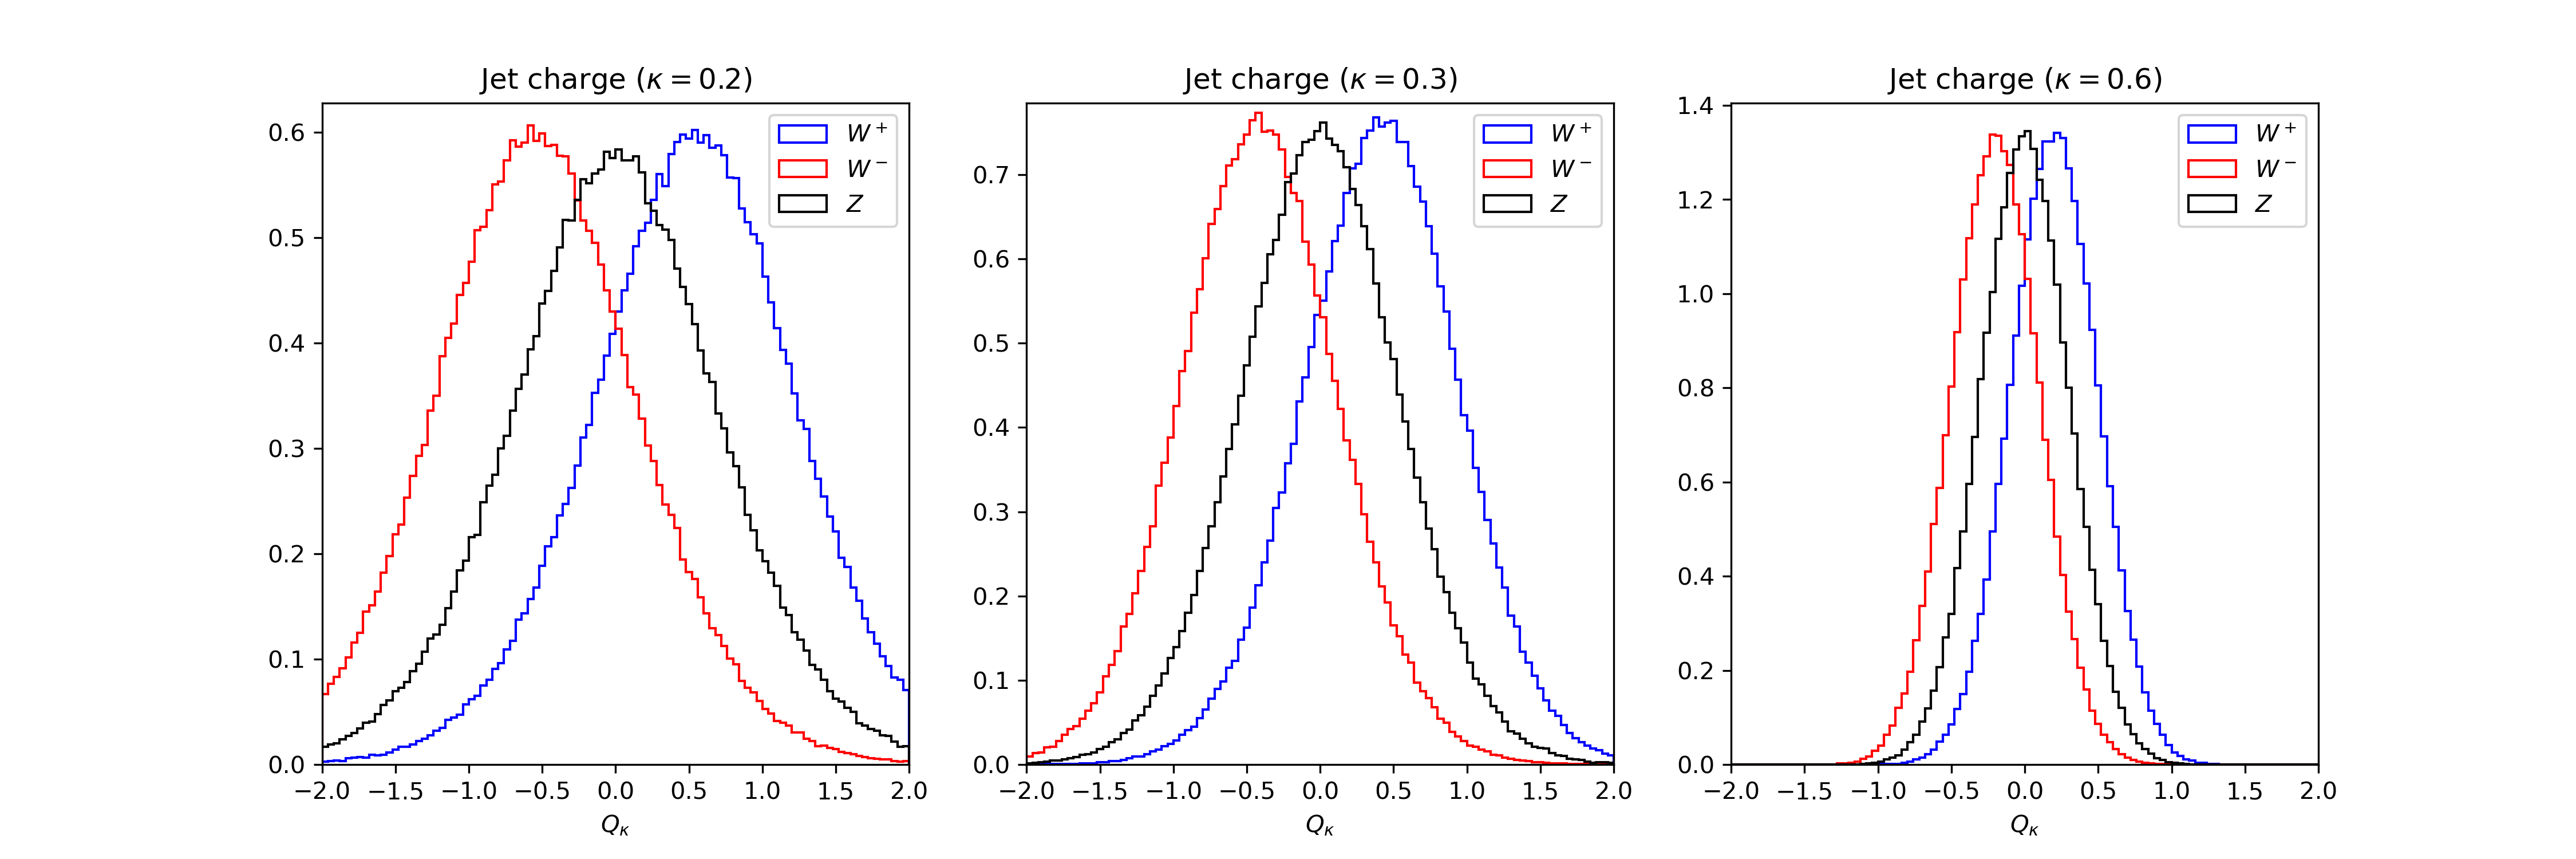
\includegraphics[width=0.95\textwidth]{jet_charge_distribution.png}
			\caption{$\mathcal{Q}_\kappa$ distributions of vector boson samples.}
			\label{fig:jet_charge_different_kappa}
		\end{figure}

		Figure \ref{fig:jet_image_PT}, \ref{fig:jet_image_Qk} are the average jet images of $p_\text{T}$ and $\mathcal{Q}_\kappa$.
		\begin{figure}[htpb]
			\centering
			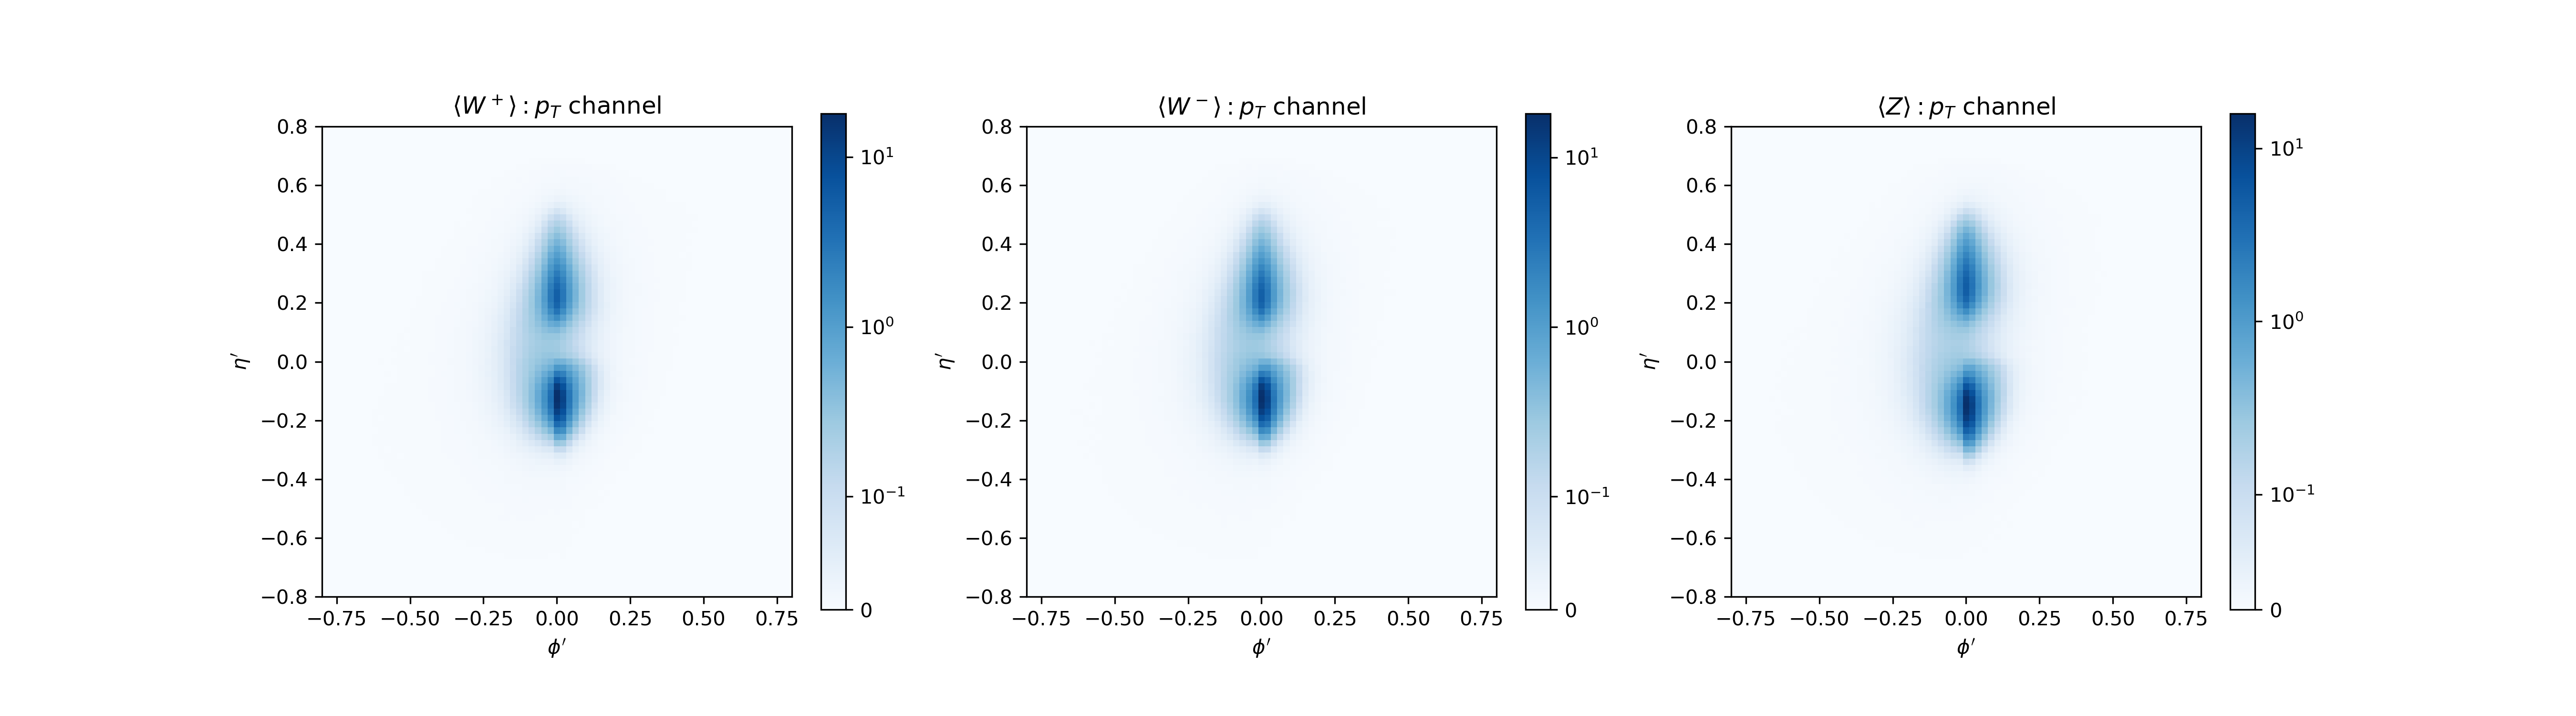
\includegraphics[width=0.95\textwidth]{jet_image_PT.png}
			\caption{Average of jet images in the $p_\text{T}$ channel.}
			\label{fig:jet_image_PT}
		\end{figure}
		\begin{figure}[htpb]
			\centering
			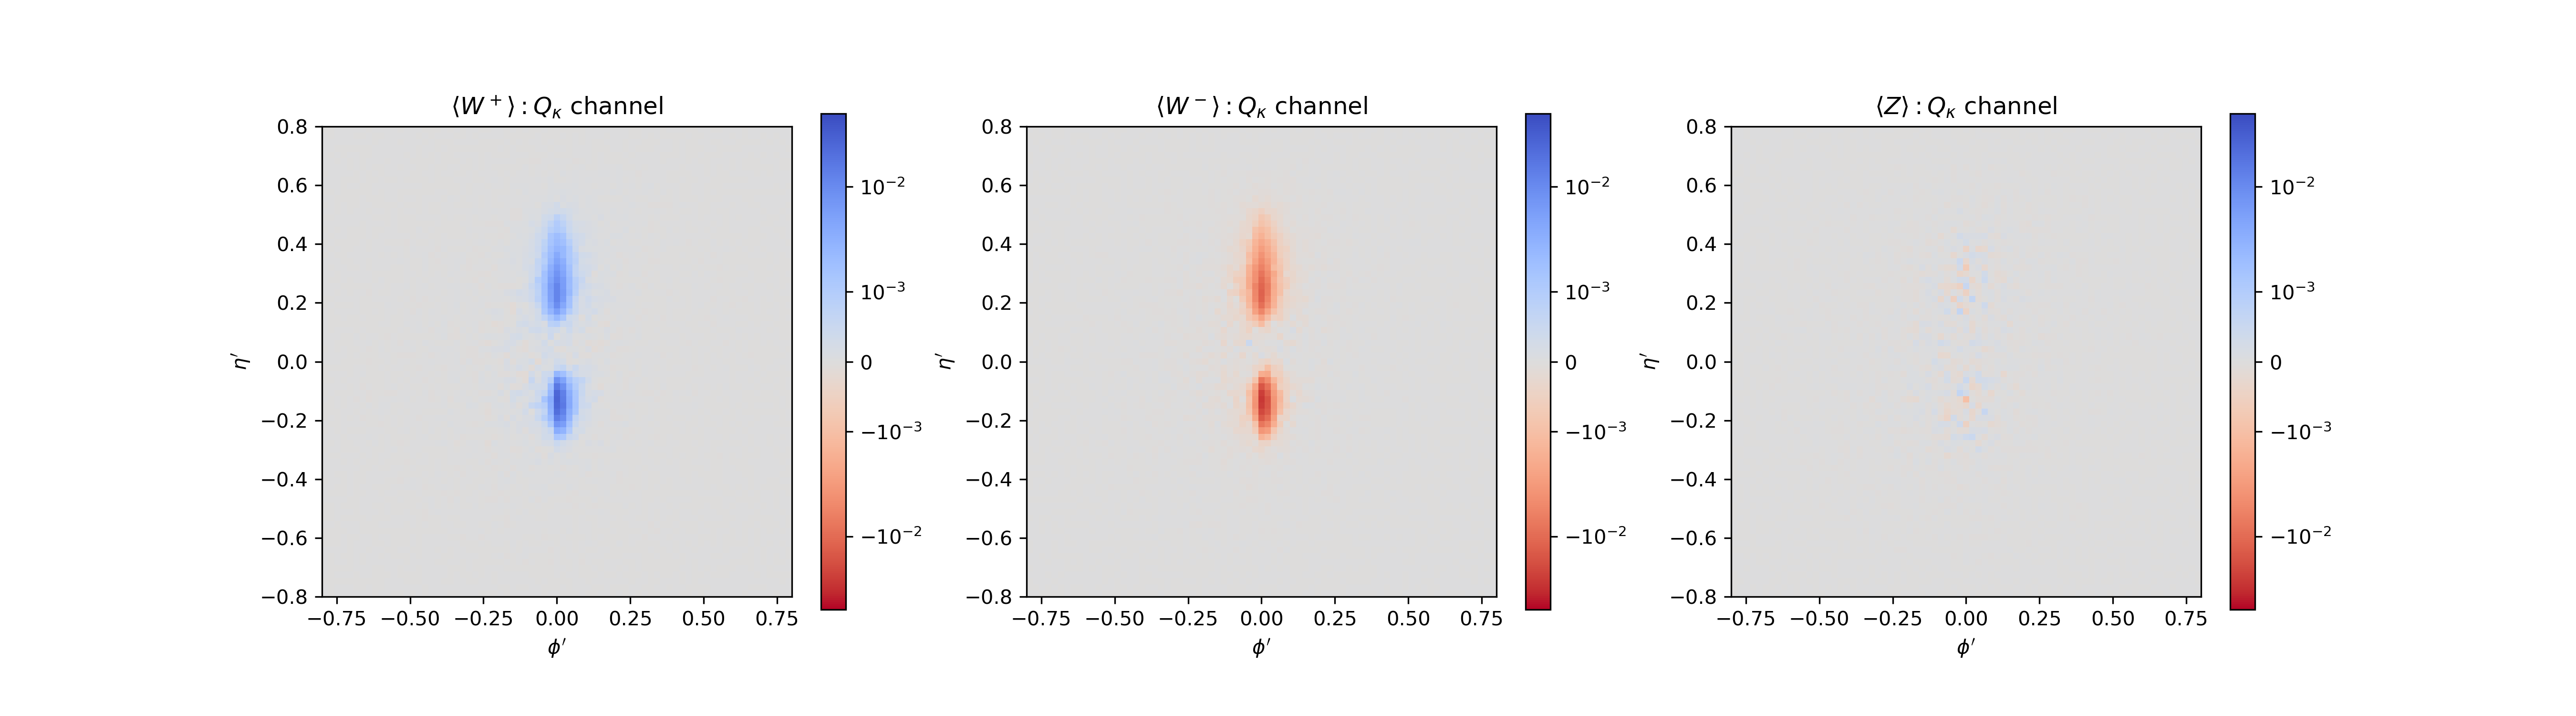
\includegraphics[width=0.95\textwidth]{jet_image_Qk.png}
			\caption{Average of jet images in the $\mathcal{Q}_\kappa$ channel, with $\kappa = 0.15$.}
			\label{fig:jet_image_Qk}
		\end{figure}
		Figure \ref{fig:jet_image_PT_Z-W+} is the $Z$ jet image minus $W^{+}$ jet image in $p_\text{T}$ channel.
		\begin{figure}[htpb]
			\centering
			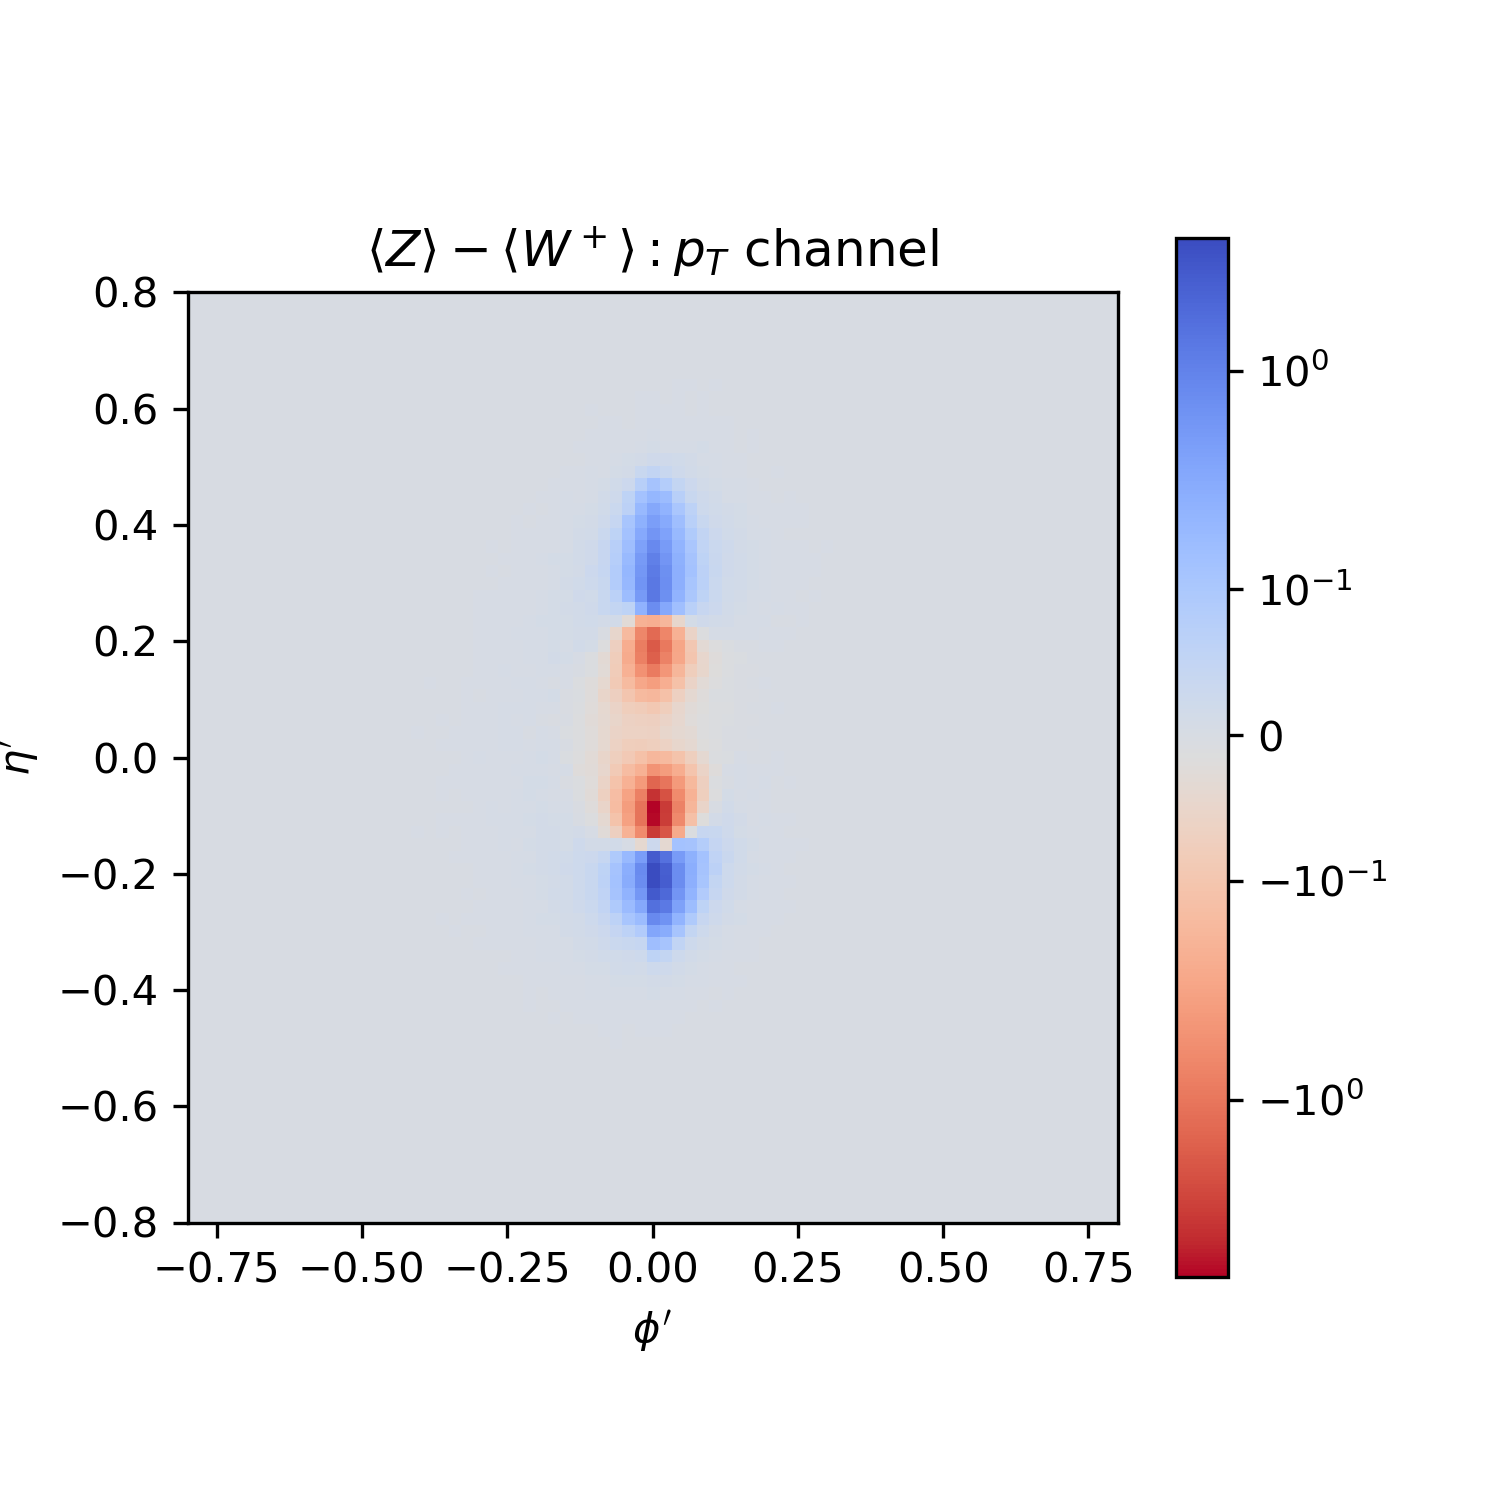
\includegraphics[width=0.5\textwidth]{jet_image_PT_Z-W+.png}
			\caption{The difference between the $Z$ and $W^{+}$ average jet images in $p_\text{T}$ channel.}
			\label{fig:jet_image_PT_Z-W+}
		\end{figure}

	% subsection plots (end)		

% section sample (end)
\section{BDT}% (fold)
\label{sec:bdt}
	The input features are jet mass $\mathcal{M}$ and jet charge $\mathcal{Q}_\kappa$.

	\subsection{BDT training}% (fold)
	\label{sub:bdt_training}
		Use the GBDT implemented by scikit-learn. The parameters are set as the default setting in sklearn.

		The training and testing sample size are in Table \ref{tab:BDT_sample_size}.
		\begin{table}[htpb]
			\centering
			\caption{The entries in the sum correspond to the $(W^{+}, W^{-}, Z)$ samples.}
			\label{tab:BDT_sample_size}
			\begin{tabular}{c|c|c}
			Case & Training set    & Testing set   \\ \hline
			1    & $14k+15k+13k$   & $3k+3k+3k$    \\
			2    & $100k+105k+90k$ & $25k+26k+22k$ \\
			3    & $242k+257k+221k$& $60k+64k+54k$ \\
			\end{tabular}
		\end{table}
	% subsection bdt_training (end)

	\subsection{BDT results}% (fold)
	\label{sub:bdt_results}
		The training results are summarized in Table \ref{tab:BDT_training_result}. The ROC of BDT for $\kappa = 0.3$ is presented in Figure \ref{fig:ROC_of_BDT}. 
		\begin{table}[htpb]
			\centering
			\caption{The training results of BDT for different $\kappa$ samples.}
			\label{tab:BDT_training_result}
			\begin{tabular}{c|c|c|cc|cc|cc}
								  &					 &             & \multicolumn{2}{c|}{$W^{+}$} & \multicolumn{2}{c|}{$W^{-}$} & \multicolumn{2}{c}{$Z$} \\
								  & Sample			 & Overall ACC & AUC		  & ACC			 & AUC          & ACC		   & AUC        & ACC       \\ \hline
			    BDT $\kappa=0.15$ &\multirow{2}{*}{1}& 0.644 & 0.808 & 0.773 & 0.812 & 0.766 & 0.812 & 0.770 \\ 
				BDT $\kappa=0.30$ &                  & 0.649 & 0.822 & 0.778 & 0.822 & 0.769 & 0.814 & 0.773 \\ \hline
			    BDT $\kappa=0.15$ &\multirow{2}{*}{2}& 0.646 & 0.808 & 0.769 & 0.815 & 0.765 & 0.809 & 0.774 \\ 
			    BDT $\kappa=0.30$ &					 & 0.652 & 0.820 & 0.774 & 0.826 & 0.772 & 0.810 & 0.775 \\ \hline
			    BDT $\kappa=0.15$ &\multirow{2}{*}{3}& 0.648 & 0.811 & 0.769 & 0.817 & 0.767 & 0.810 & 0.775 \\ 
			    BDT $\kappa=0.30$ &					 & 0.654 & 0.824 & 0.776 & 0.829 & 0.773 & 0.811 & 0.774 \\
			\end{tabular}
		\end{table}

		\begin{figure}[htpb]
			\centering
			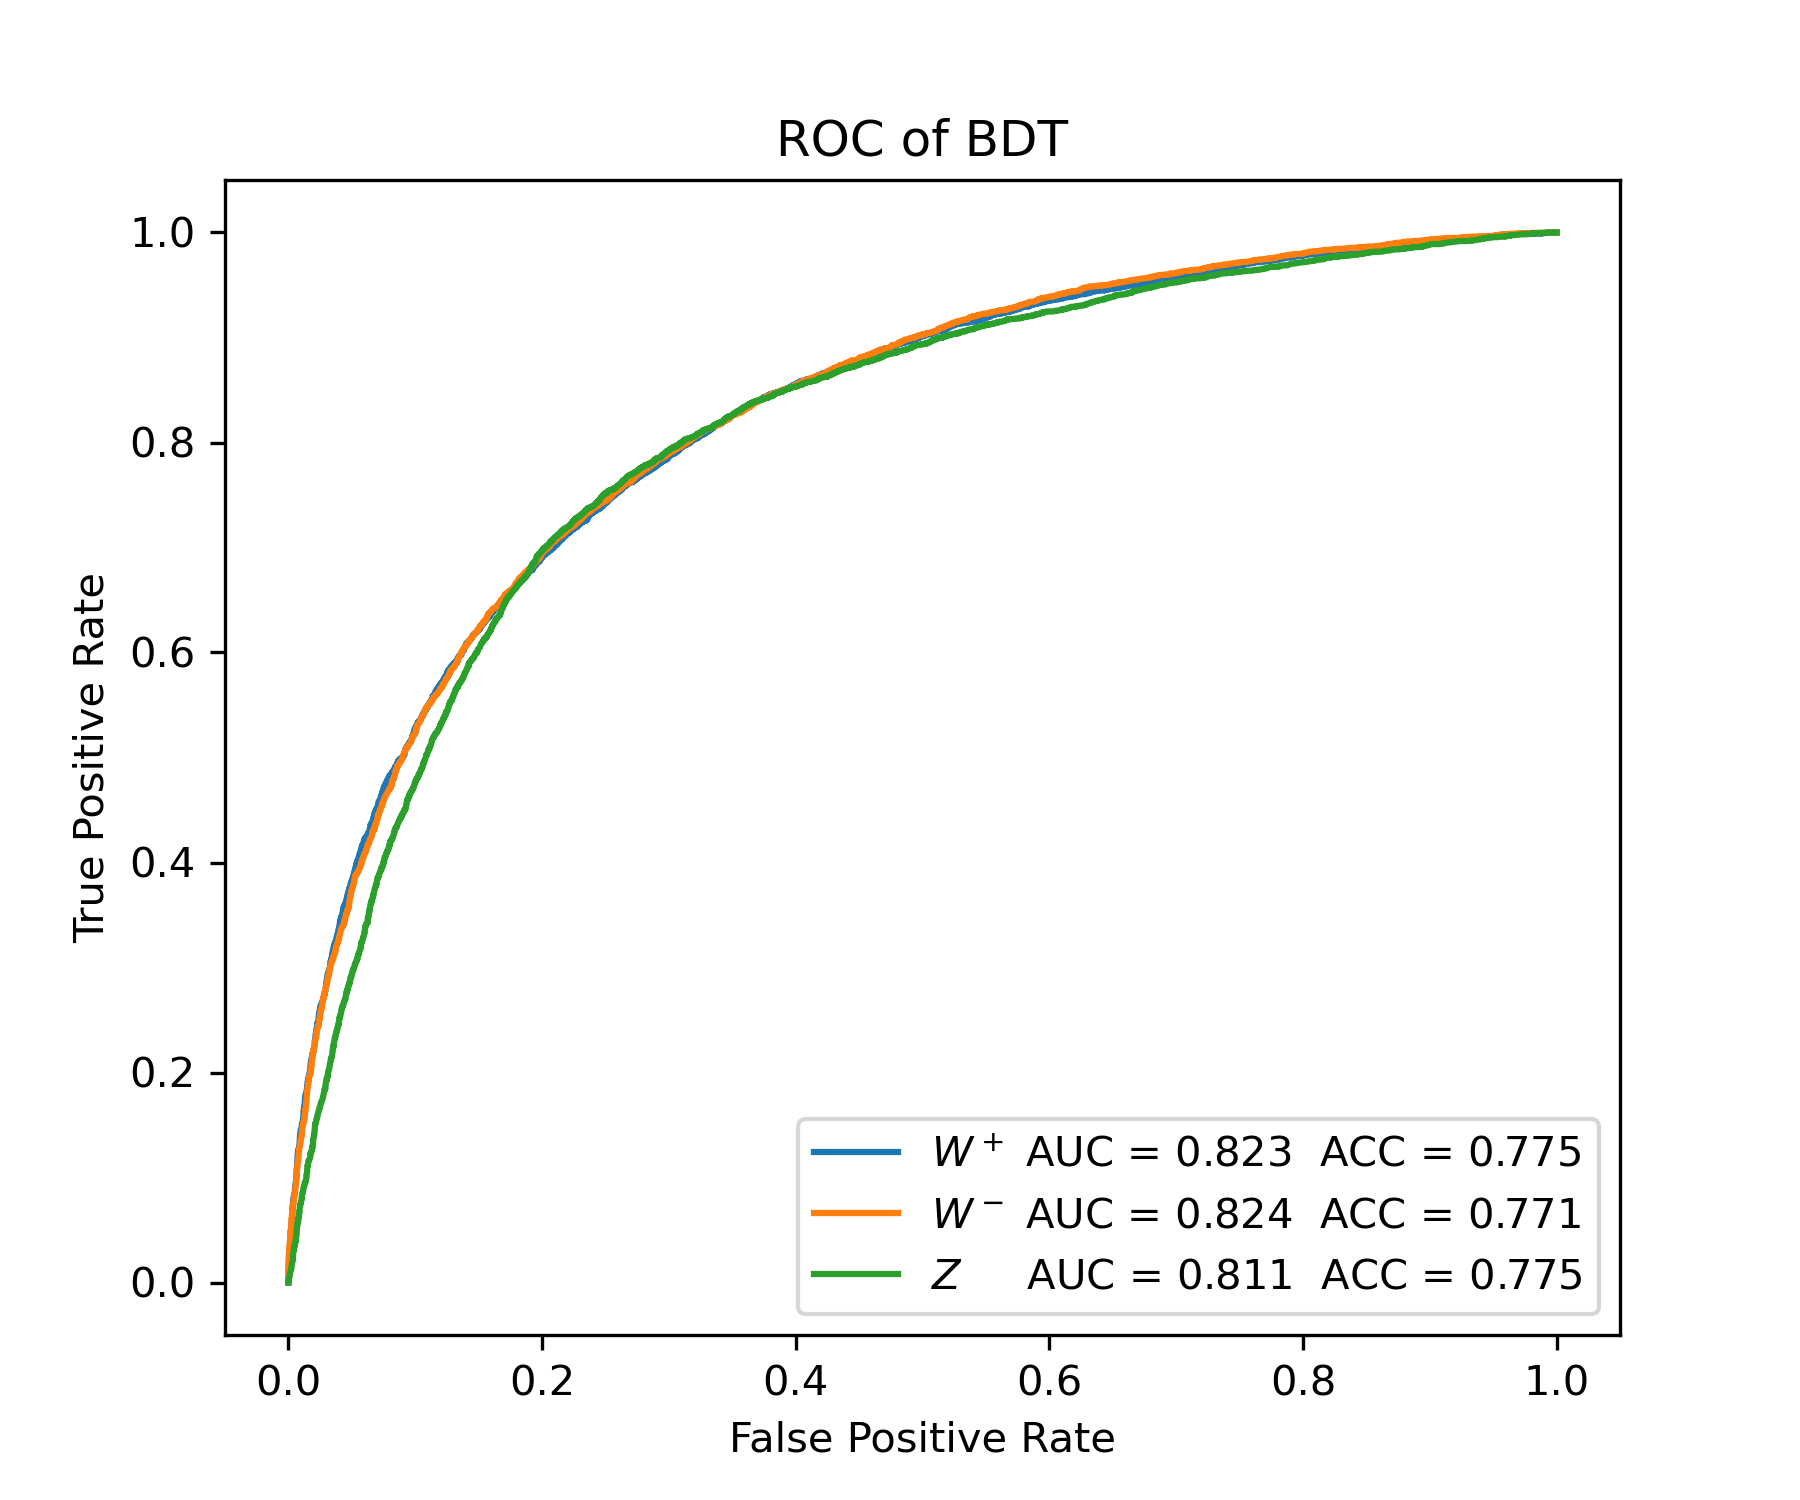
\includegraphics[width=0.8\textwidth]{ROC_BDT.png}
			\caption{The ROC of BDT. Case $W^{+}$ means take $W^{+}$ samples as signal and $W^{-}, Z$ as background.}
			\label{fig:ROC_of_BDT}
		\end{figure}

		\begin{figure}[htpb]
			\centering
			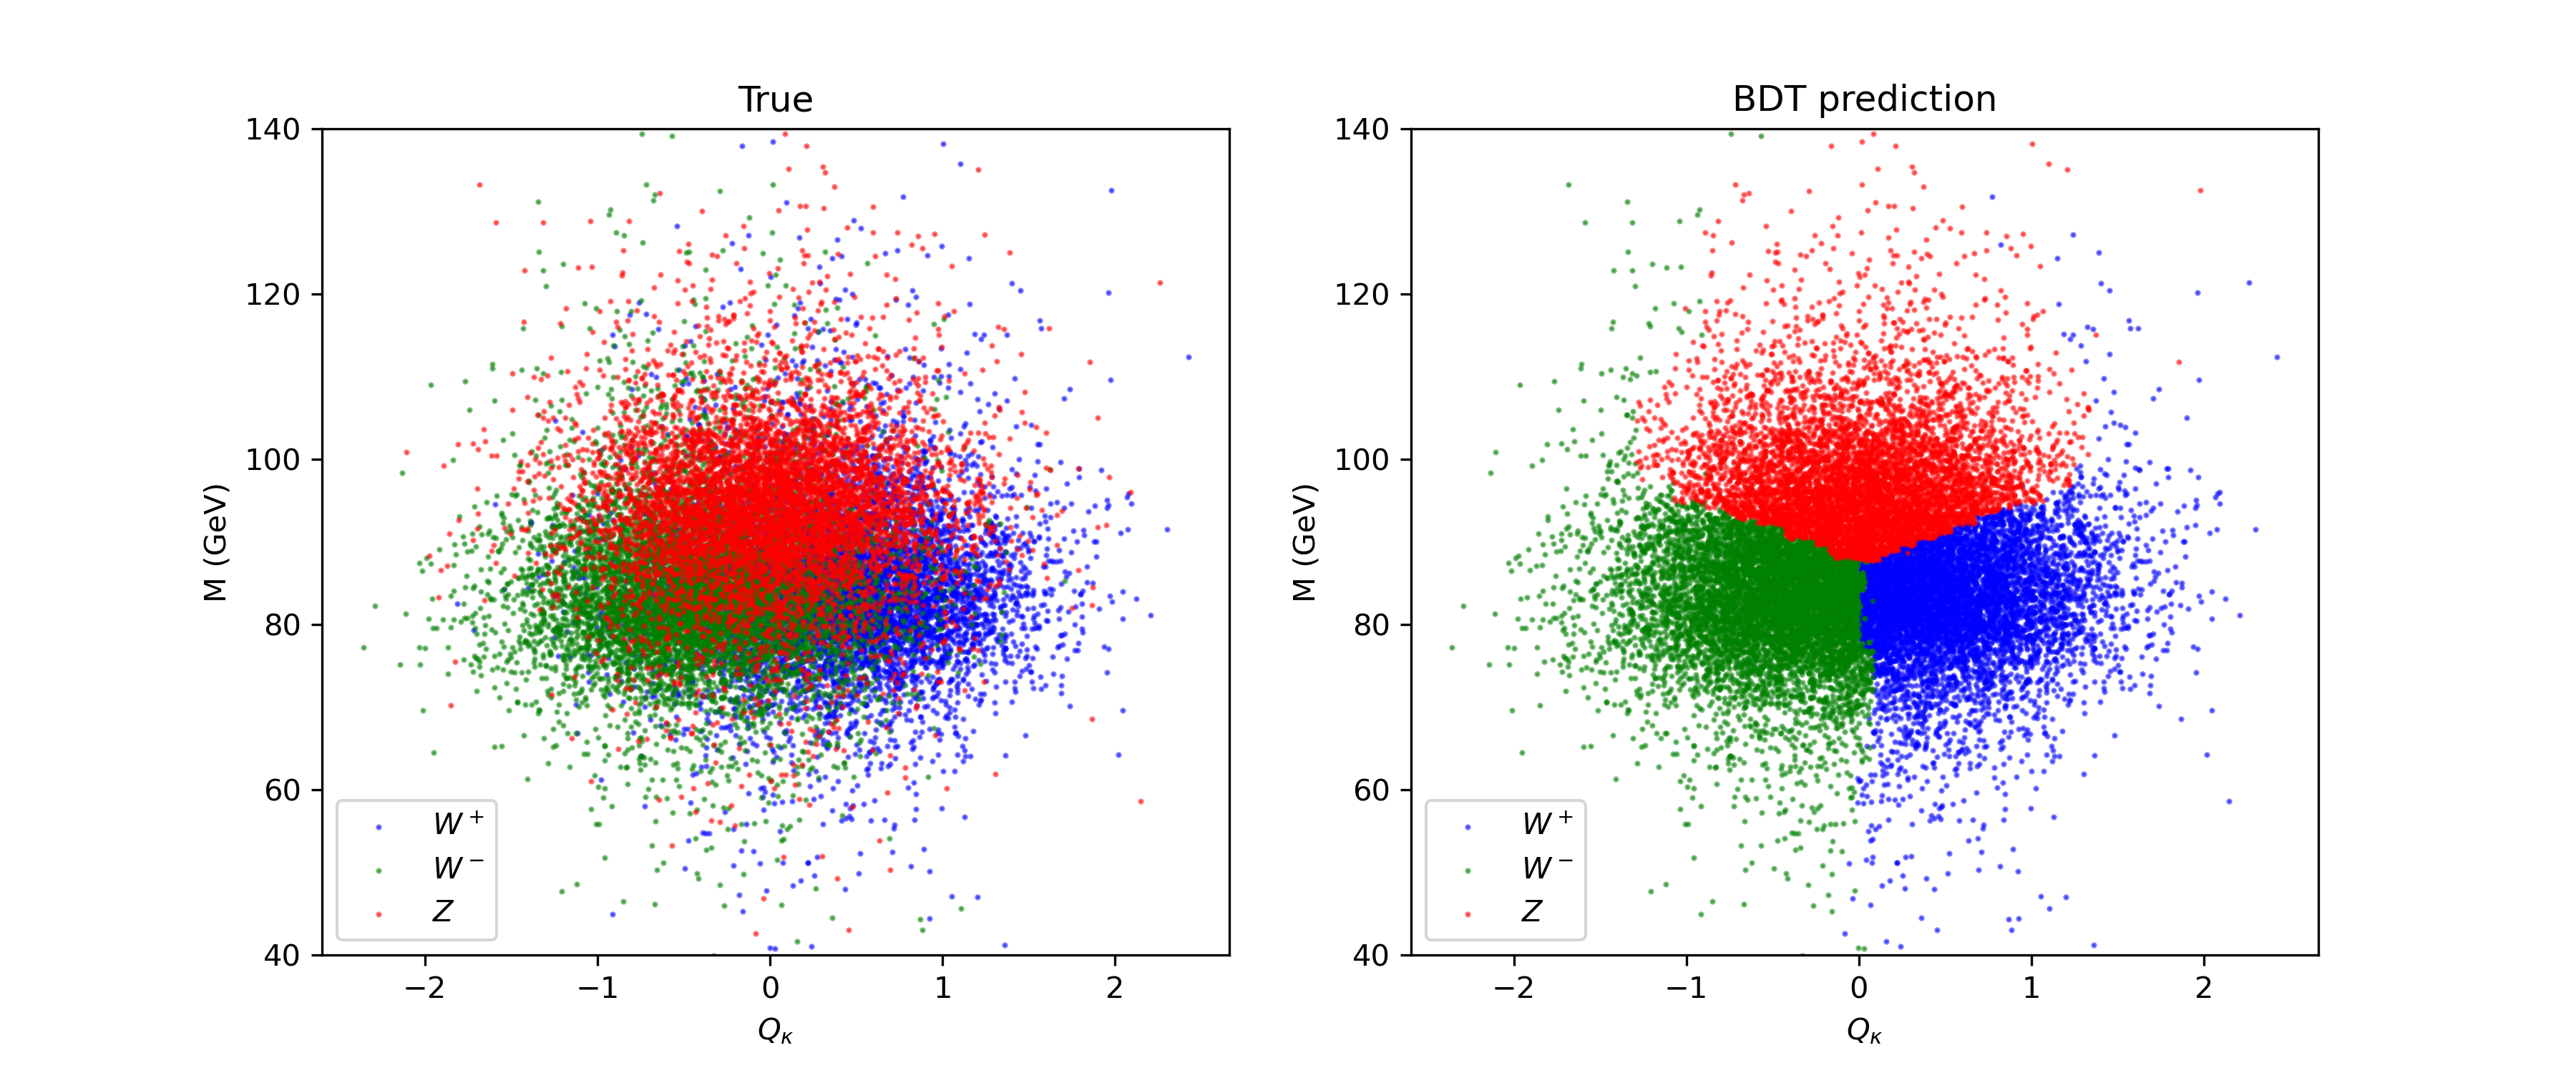
\includegraphics[width=0.9\textwidth]{figures/True_and_BDT_distribution_of_M_Qk.png}
			\caption{The left plot shows the true distributions for $W^{+}, W^{-}, Z$  in the $(\mathcal{Q}_\kappa ,\mathcal{M})$ plane (for $\kappa=0.3$). The right plot is the BDT prediction.}
			\label{fig:M_Qk_distribution}
		\end{figure}

		% subsection bdt_results (end)
% section bdt (end)	
\section{CNN}% (fold)
\label{sec:cnn}
	The inputs are the jet image of $p_T$ and $\mathcal{Q}_\kappa$.
	\subsection{CNN training}% (fold)
	\label{sub:cnn_training}
		The training, validation, and testing sample size are in Table \ref{tab:CNN_sample_size}.
		\begin{table}[htpb]
			\centering
			\caption{The entries in the sum correspond to the $(W^{+}, W^{-}, Z)$ samples.}
			\label{tab:CNN_sample_size}
			\begin{tabular}{c|c|c|c}
			Case & Training set     & Validation set & Testing set   \\ \hline
			1    & $11k+12k+10k$    & $2k+2k+2k$     & $3k+3k+3k$    \\
			2    & $80k+84k+72k$    & $19k+21k+18k$  & $25k+26k+22k$ \\
			3    & $194k+205k+176k$ & $48k+51k+44k$  & $60k+64k+55k$
			\end{tabular}
		\end{table}
	% subsection cnn_training (end)
	\subsection{CNN results}% (fold)
	\label{sub:cnn_results}
		The training results are summarized in Table \ref{tab:CNN_training_result}. The ROC of CNN for $\kappa = 0.15$ is presented in Figure \ref{fig:CNN_of_BDT}.
		\begin{table}[htpb]
			\centering
			\caption{The training results of CNN with different $\kappa$ samples.}
			\label{tab:CNN_training_result}
			\begin{tabular}{c|c|c|cc|cc|cc}
								  &					  &             & \multicolumn{2}{c|}{$W^{+}$} & \multicolumn{2}{c|}{$W^{-}$} & \multicolumn{2}{c}{$Z$} \\
								  & Sample			  & Overall ACC & AUC        & ACC       & AUC        & ACC       & AUC       & ACC       \\ \hline
				CNN $\kappa=0.15$ & \multirow{2}{*}{1}& 0.639 & 0.825 & 0.772 & 0.829 & 0.774 & 0.782 & 0.768 \\
				CNN $\kappa=0.30$ &					  & 0.632 & 0.822 & 0.771 & 0.825 & 0.771 & 0.786 & 0.771 \\ \hline
				CNN $\kappa=0.15$ & \multirow{2}{*}{2}& 0.667 & 0.847 & 0.790 & 0.847 & 0.784 & 0.828 & 0.795 \\
				CNN $\kappa=0.30$ &					  & 0.663 & 0.843 & 0.786 & 0.843 & 0.779 & 0.825 & 0.795 \\ \hline
				CNN $\kappa=0.15$ & \multirow{2}{*}{3}& 0.672 & 0.849 & 0.793 & 0.851 & 0.787 & 0.834 & 0.799 \\
				CNN $\kappa=0.30$ &					  & 0.666 & 0.845 & 0.788 & 0.847 & 0.783 & 0.832 & 0.800 \\
			\end{tabular}
		\end{table}	
		\begin{figure}[htpb]
			\centering
			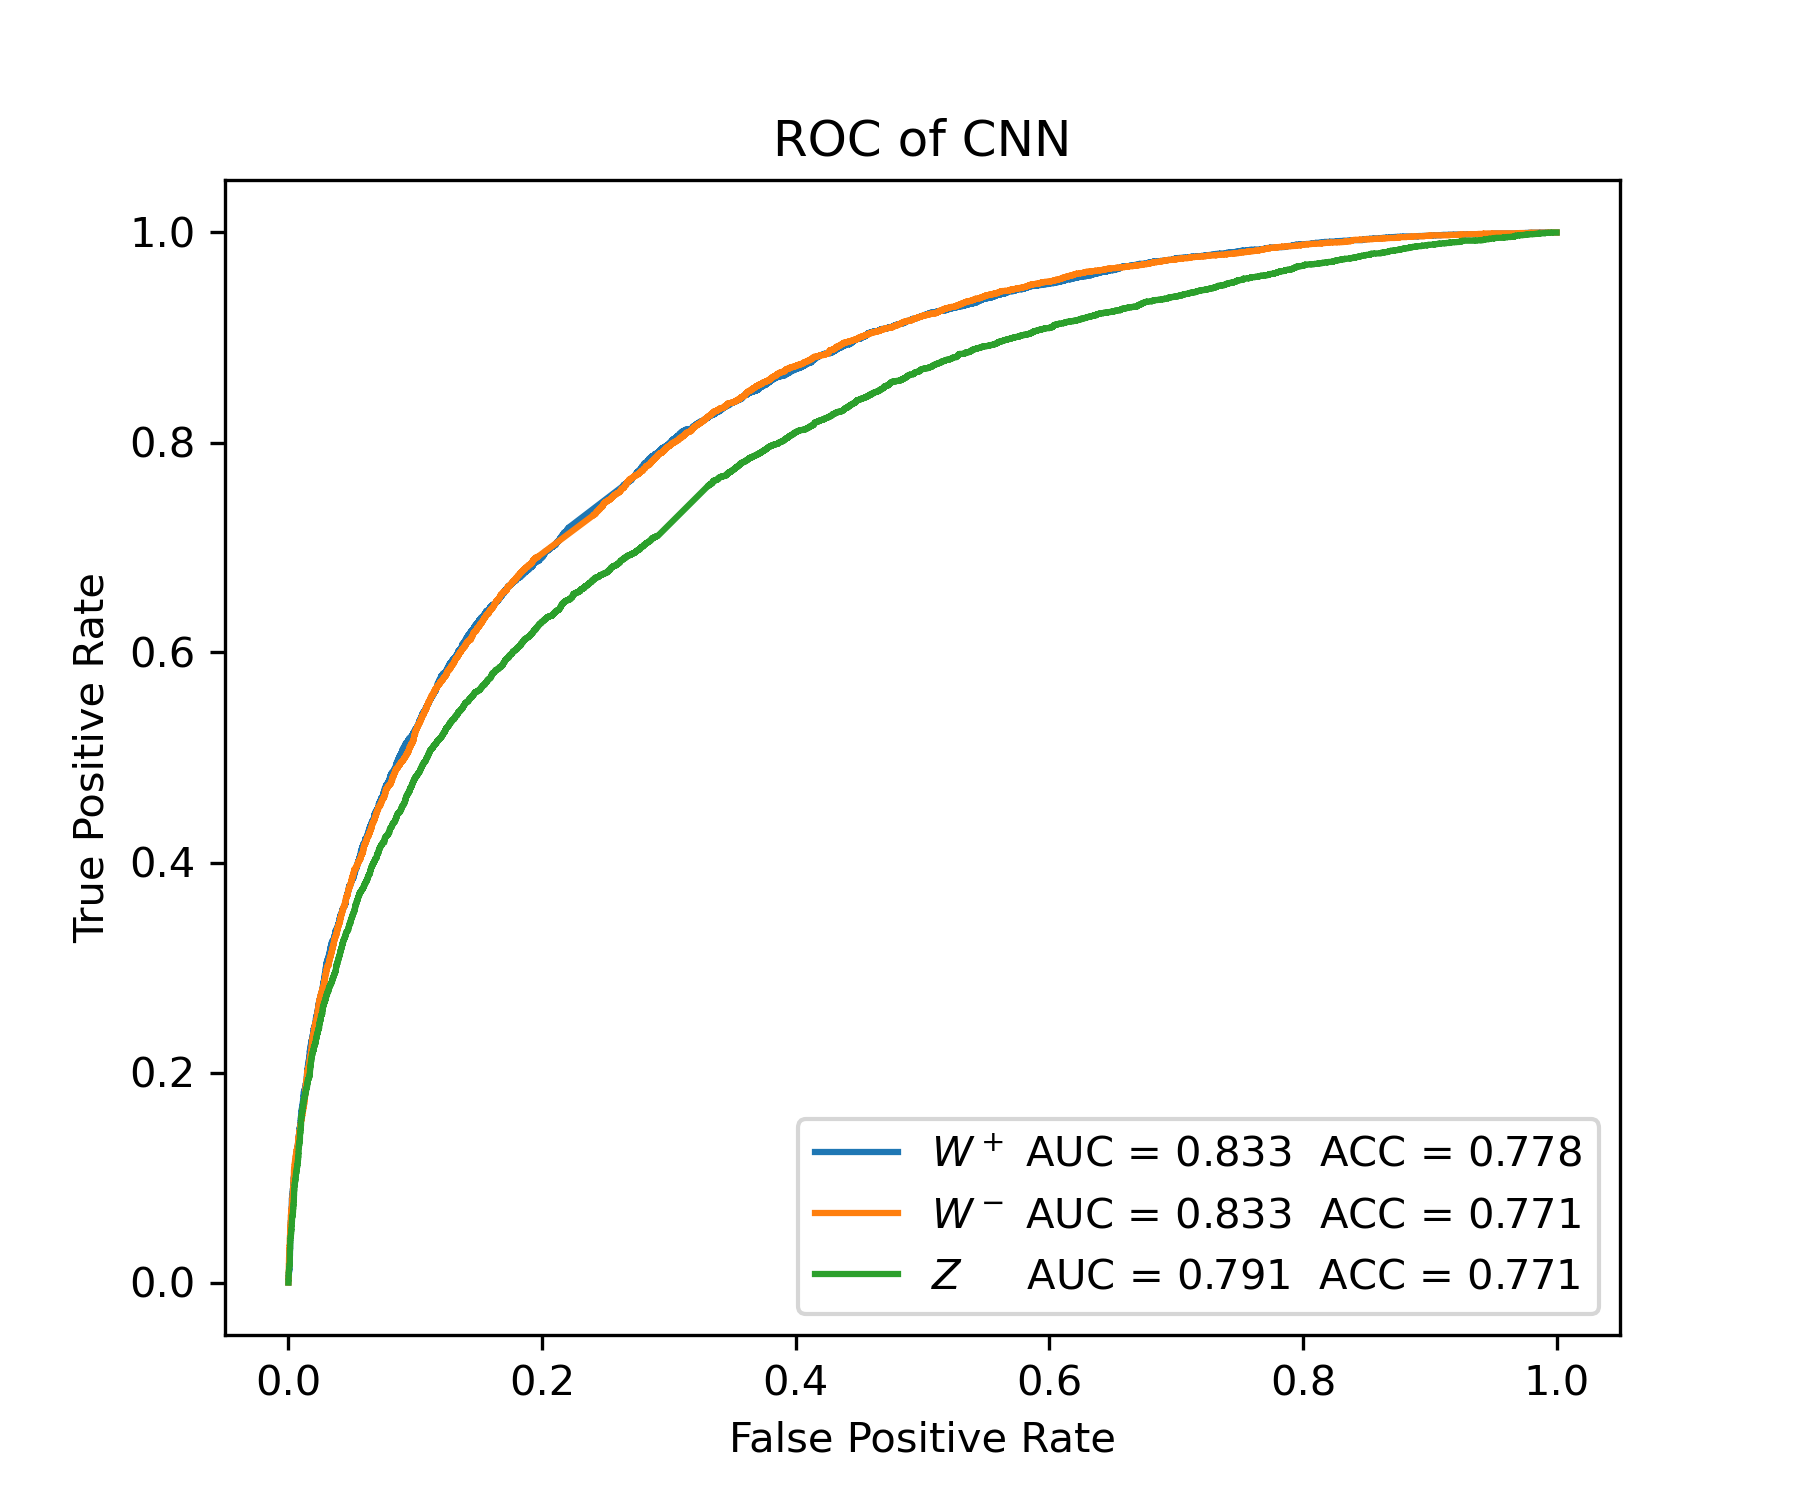
\includegraphics[width=0.8\textwidth]{ROC_CNN.png}
			\caption{The ROC of CNN for $\kappa = 0.15$. Case $W^{+}$ means take $W^{+}$ samples as signal and $W^{-}, Z$ as background.}
			\label{fig:CNN_of_BDT}
		\end{figure}
		
	% subsection cnn_results (end)	
% section CNN (end)		
\section{CNN\texorpdfstring{$^2$}{2}}% (fold)
\label{sec:cnn2}
	\subsection{CNN\texorpdfstring{$^2$}{2} training}% (fold)
	\label{sub:cnn2_training}
		The training, validation, and testing sample size are in Table \ref{tab:CNNsq_sample_size}.
		\begin{table}[htpb]
			\centering
			\caption{The entries in the sum correspond to the $(W^{+}, W^{-}, Z)$ samples.}
			\label{tab:CNNsq_sample_size}
			\begin{tabular}{c|c|c|c}
			Case & Training set     & Validation set & Testing set   \\ \hline
			1    & $11k+12k+10k$    & $2k+2k+2k$     & $3k+3k+3k$    \\
			2    & $80k+84k+72k$    & $19k+21k+18k$  & $25k+26k+22k$ \\
			3    & $194k+205k+176k$ & $48k+51k+44k$  & $60k+64k+55k$
			\end{tabular}
		\end{table}

	% subsection cnn2_training (end)
	\subsection{CNN\texorpdfstring{$^2$}{2} results}% (fold)
	\label{sub:cnn2_results}
		The training results are summarized in Table \ref{tab:CNNsq_training_result}.
		\begin{table}[htpb]
			\centering
			\caption{The training results of $\text{CNN}^2$ for different $\kappa$ samples.}
			\label{tab:CNNsq_training_result}
			\begin{tabular}{c|c|c|cc|cc|cc}
								  &					  &             & \multicolumn{2}{c|}{$W^{+}$} & \multicolumn{2}{c|}{$W^{-}$} & \multicolumn{2}{c}{$Z$} \\
								  & Sample			  & Overall ACC & AUC        & ACC       & AUC        & ACC       & AUC       & ACC       \\ \hline
			$\text{CNN}^2$ $\kappa=0.15$ & \multirow{2}{*}{1}& 0.642 & 0.828 & 0.773 & 0.831 & 0.773 & 0.801 & 0.780 \\
			$\text{CNN}^2$ $\kappa=0.30$ &					 & 0.645 & 0.823 & 0.773 & 0.828 & 0.773 & 0.802 & 0.784 \\ \hline
			$\text{CNN}^2$ $\kappa=0.15$ & \multirow{2}{*}{2}& 0.677 & 0.848 & 0.792 & 0.848 & 0.786 & 0.842 & 0.806 \\
			$\text{CNN}^2$ $\kappa=0.30$ &					 & 0.669 & 0.842 & 0.788 & 0.843 & 0.780 & 0.839 & 0.804 \\ \hline
			$\text{CNN}^2$ $\kappa=0.15$ & \multirow{2}{*}{3}& 0.674 & 0.848 & 0.792 & 0.849 & 0.785 & 0.843 & 0.807 \\
			$\text{CNN}^2$ $\kappa=0.30$ &					 & 0.675 & 0.846 & 0.790 & 0.847 & 0.784 & 0.845 & 0.808 \\
			\end{tabular}
		\end{table}	
		
	% subsection cnn2_results (end)	
% section cnn2 (end)		
\section{Modify preprocess and preselection}% (fold)
\label{sec:modify_preprocess_and_preselection}
	Preprocess: For the vector boson jet which $\phi$ coordinate across the $\phi = \pm\pi$ boundary, plus its $\phi$ coordinate by  $\pi$ such that its center is located around $\phi = 0$.

	Preselection: Include the events with only one jet that can pass the cuts.

	\subsection{CNN results for modified preprocess and preselection}% (fold)
	\label{sub:cnn_results_for_modified_preprocess_and_preselection}
		The training, validation, and testing sample size are in Table \ref{tab:CNN_sample_size_modified}.
		\begin{table}[htpb]
			\centering
			\caption{The entries in the sum correspond to the $(W^{+}, W^{-}, Z)$ samples.}
			\label{tab:CNN_sample_size_modified}
			\begin{tabular}{c|c|c|c}
			Case & Training set     & Validation set & Testing set   \\ \hline
			1    & $313k+323k+307k$ & $78k+80k+76k$  & $97k+100k+96k$ \\
			\end{tabular}
		\end{table}

		The training results are summarized in Table \ref{tab:CNN_training_result_modified}.
		\begin{table}[htpb]
			\centering
			\caption{The training results of CNN with modified preprocessing and preselection.}
			\label{tab:CNN_training_result_modified}
			\begin{tabular}{c|c|c|cc|cc|cc}
								  &					  &             & \multicolumn{2}{c|}{$W^{+}$} & \multicolumn{2}{c|}{$W^{-}$} & \multicolumn{2}{c}{$Z$} \\
								  & Sample			  & Overall ACC & AUC        & ACC       & AUC        & ACC       & AUC       & ACC       \\ \hline
				CNN $\kappa=0.15$ & \multirow{1}{*}{1}& 0.684 & 0.857 & 0.798 & 0.855 & 0.794 & 0.828 & 0.793\\
				CNN${}^2$ $\kappa=0.15$ & \multirow{1}{*}{1}& 0.684 & 0.855 & 0.797 & 0.854 & 0.793 & 0.835 & 0.797\\
			\end{tabular}
		\end{table}	

	% subsection cnn_results_for_modified_preprocess_and_preselection (end)
	\subsection{CNN results for Fishbone}% (fold)
	\label{sub:cnn_results_for_fishbone}
		The training, validation, and testing sample size are in Table \ref{tab:CNN_sample_size_fish}. For case 1, only consider the events with 2 jets that can pass the cuts. For case 2, the events with only 1 jet can pass the cuts are included. 
		\begin{table}[htpb]
			\centering
			\caption{The entries in the sum correspond to the $(W^{+}, W^{-}, Z)$ samples.}
			\label{tab:CNN_sample_size_fish}
			\begin{tabular}{c|c|c|c}
			Case & Training set     & Validation set & Testing set   \\ \hline
			1    & $61k+65k+102k$ & $15k+16k+25k$ & $19k+20k+32k$\\
			2    & $313k+323k+307k$ & $78k+81k+76k$ & $97k+101k+95k$ \\
			\end{tabular}
		\end{table}
		The training results are summarized in Table \ref{tab:CNN_training_result_fish}.
		\begin{table}[htpb]
			\centering
			\caption{The training results of CNN with Fishbone's code.}
			\label{tab:CNN_training_result_fish}
			\begin{tabular}{c|c|c|cc|cc|cc}
								  &					  &             & \multicolumn{2}{c|}{$W^{+}$} & \multicolumn{2}{c|}{$W^{-}$} & \multicolumn{2}{c}{$Z$} \\
								  & Sample			  & Overall ACC & AUC        & ACC       & AUC        & ACC       & AUC       & ACC       \\ \hline
				CNN $\kappa=0.15$ & \multirow{1}{*}{1}& 0.694 & 0.857 & 0.820 & 0.856 & 0.814 & 0.842 & 0.776 \\
				CNN $\kappa=0.15$ & \multirow{1}{*}{2}& 0.682 & 0.856 & 0.797 & 0.854 & 0.793 & 0.827 & 0.791 \\
			\end{tabular}
		\end{table}

	% subsection cnn_results_for_fishbone (end)	
% section modify_preprocess_and_preselection (end)		
\section{Old sample for training}% (fold)
\label{sec:old_sample_for_training}
	This section uses the model \verb+GM_UFO+ and different parameter settings. The model and parameters are the same as the paper. The selection criteria are the same as Sec.\ref{sub:sample_selection}. The events with only one vector boson passing the criteria are included.

	Following are the MadGraph scripts for generating $W^{+}$ sample:
	\begin{verbatim}
	import model GM_UFO
	define v = z w+ w-
	generate p p > H5pp j j $$v, (H5pp > w+ w+, (w+ > j j), (w+ > j j))
	output VBF_H5pp_ww_jjjj-J

	launch VBF_H5pp_ww_jjjj-J

	shower=Pythia8
	detector=Delphes
	analysis=OFF
	done

	set param_card tanth 2.234400e+01
	set param_card lam2 1.040100e+00
	set param_card lam3 8.829540e+00
	set param_card lam4 -2.232270e+00
	set param_card lam5 7.672600e+00
	set param_card M1coeff 1.000000e+02
	set param_card M2coeff 1.000000e+02

	set param_card wt 1.000000e+00
	set param_card wz 1.000000e+00
	set param_card ww 1.000000e+00
	set param_card wh Auto
	set param_card wh__2 Auto
	set param_card wh3p Auto
	set param_card wh3z Auto
	set param_card wh5pp Auto
	set param_card wh5p Auto
	set param_card wh5z Auto

	set run_card nevents 10000
	set run_card ebeam1 6500.0
	set run_card ebeam2 6500.0

	/home/r10222035/boosted_V_ML_test/Cards/delphes_card.dat

	done
	\end{verbatim}

	\subsection{Training results}% (fold)
	\label{sub:training_results}
		The training, validation, and testing sample size are in Table \ref{tab:sample_size_old}.
		\begin{table}[htpb]
			\centering
			\caption{The entries in the sum correspond to the $(W^{+}, W^{-}, Z)$ samples.}
			\label{tab:sample_size_old}
			\begin{tabular}{c|c|c|c}
			Case & Training set     & Validation set & Testing set   \\ \hline
			1    & $112k+116k+101k$ & $27k+29k+25k$ & $34k+36k+31k$ \\
			2    & $224k+232k+201k$ & $56k+58k+50k$ & $69k+72k+63k$ \\
			\end{tabular}
		\end{table}

		The training results are summarized in Table \ref{tab:training_result_old}.
		\begin{table}[htpb]
			\centering
			\caption{The training results of CNN with modified preprocessing and preselection.}
			\label{tab:training_result_old}
			\begin{tabular}{c|c|c|cc|cc|cc}
										&					  &             & \multicolumn{2}{c|}{$W^{+}$} & \multicolumn{2}{c|}{$W^{-}$} & \multicolumn{2}{c}{$Z$} \\
										& Sample			  & Overall ACC & AUC        & ACC       & AUC        & ACC       & AUC       & ACC       \\ \hline
				CNN $\kappa=0.15$		& \multirow{2}{*}{1}  & 0.690 & 0.861 & 0.798 & 0.858 & 0.793 & 0.830 & 0.808 \\
				CNN${}^2$ $\kappa=0.15$ &					  & 0.693 & 0.860 & 0.797 & 0.859 & 0.794 & 0.838 & 0.816 \\ \hline
				CNN $\kappa=0.15$		& \multirow{2}{*}{2}  & 0.697 & 0.864 & 0.801 & 0.863 & 0.796 & 0.837 & 0.812 \\
				CNN${}^2$ $\kappa=0.15$ &					  & 0.698 & 0.863 & 0.800 & 0.862 & 0.797 & 0.844 & 0.818 \\ \hline
			\end{tabular}
		\end{table}
		The results are better than the Sec.\ref{sub:cnn_results_for_modified_preprocess_and_preselection}.
	% subsection training_results (end)

% section old_sample_for_training (end)		
\section{Full event sample}% (fold)
\label{sec:full_event_sample}
	For the full event case, there are six processes: $H_5^{\pm\pm} \to W^{\pm}W^{\pm} \to jjjj$, $H_5^{\pm} \to W^{\pm}Z \to jjjj$, $H_5\to ZZ \to jjjj$, $H_5\to W^{+}W^{-} \to jjjj$.

	\subsection{Full event sample selection}% (fold)
	\label{sub:full_event_sample_selection}	
		Only the events that satisfy the following requirements will be used for training.
		\begin{enumerate}
			\item The transverse momentum of vector boson jets are required $p_\text{T} \in (350, 450) \text{ GeV}$ and in range $\abs{\eta}<1$.
			\item Merging: The angular distance between the two quarks decayed from the vector boson is required $\Delta R(q_1,q_2) < 0.6$.
			\item Matching: The vector boson and jet are matched if $\Delta R(V,j) < 0.1$. The events with less than two matching jets will be discarded.
		\end{enumerate}
	
	% subsection full_event_sample_selection (end)
	\subsection{Full event sample pre-processing}% (fold)
	\label{sub:full_event_sample_pre_processing}
		\subsubsection{Event image}% (fold)
		\label{subs:event_image}
			After the sample selection, we can construct the event image. The event image contains 2 vector boson jets and 2 forward jets. The vector boson jets are selected by the merging requirement. The forward jets are selected by the highest $p_\text{T}$ jets from the remaining jets. The event image is constructed by the following steps:
			\begin{enumerate}
				\item Centralization: Calculating the $p_\text{T}$ weighted center in $\phi$ coordinate, then shift this point to origin.
				\item Flipping: Flip the highest intensity quadrant to the first quadrant. 
				\item Pixelating in $\Delta\eta = \Delta\phi = 6$ box, with $75\times 75$ pixels.
			\end{enumerate}
		% subsubsection event_image (end)	
	% subsection full_event_sample_pre_processing (end)	
	\subsection{Event sample plots}% (fold)
	\label{sub:event_sample_plots}
		Figure \ref{fig:single_event_image_PT}, \ref{fig:single_event_image_Qk} are the single event images of $p_\text{T}$ and $\mathcal{Q}_\kappa$. Figure \ref{fig:event_image_PT}, \ref{fig:event_image_Qk} are the average event images of $p_\text{T}$ and $\mathcal{Q}_\kappa$.
		\begin{figure}[htpb]
			\centering
			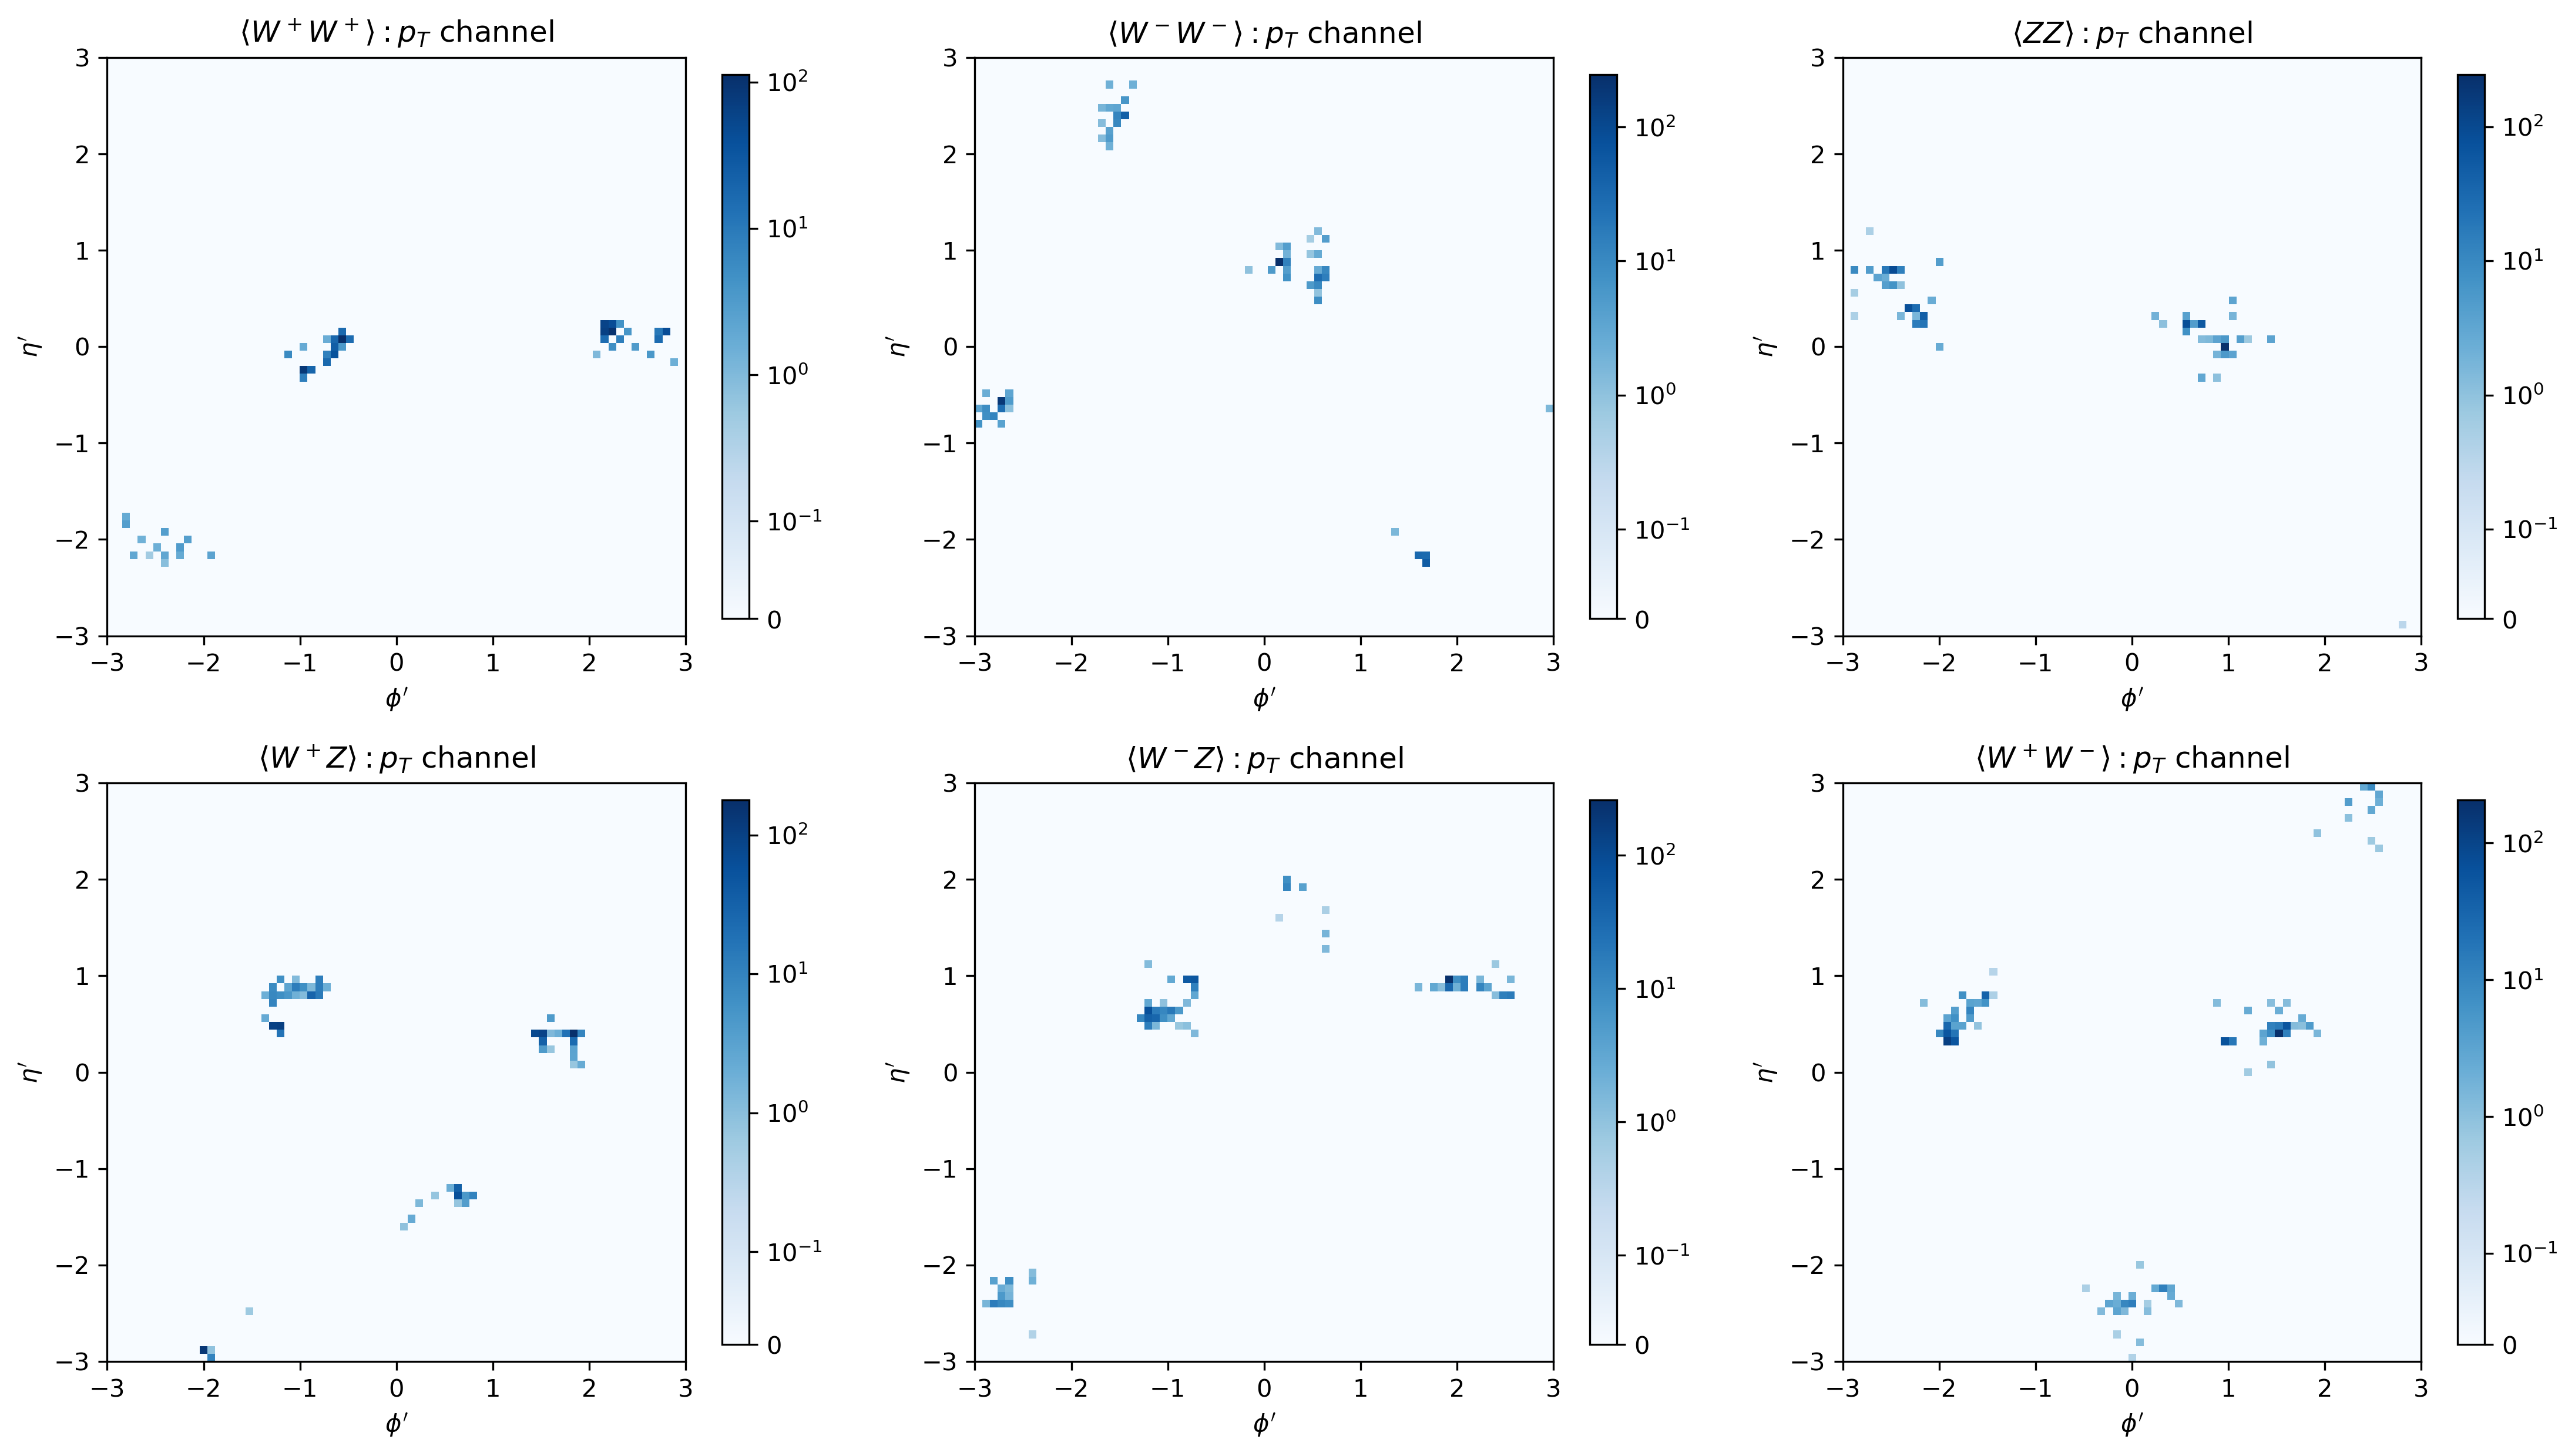
\includegraphics[width=0.95\textwidth]{single_event_image_PT.png}
			\caption{Single event images in the $p_\text{T}$ channel.}
			\label{fig:single_event_image_PT}
		\end{figure}
		\begin{figure}[htpb]
			\centering
			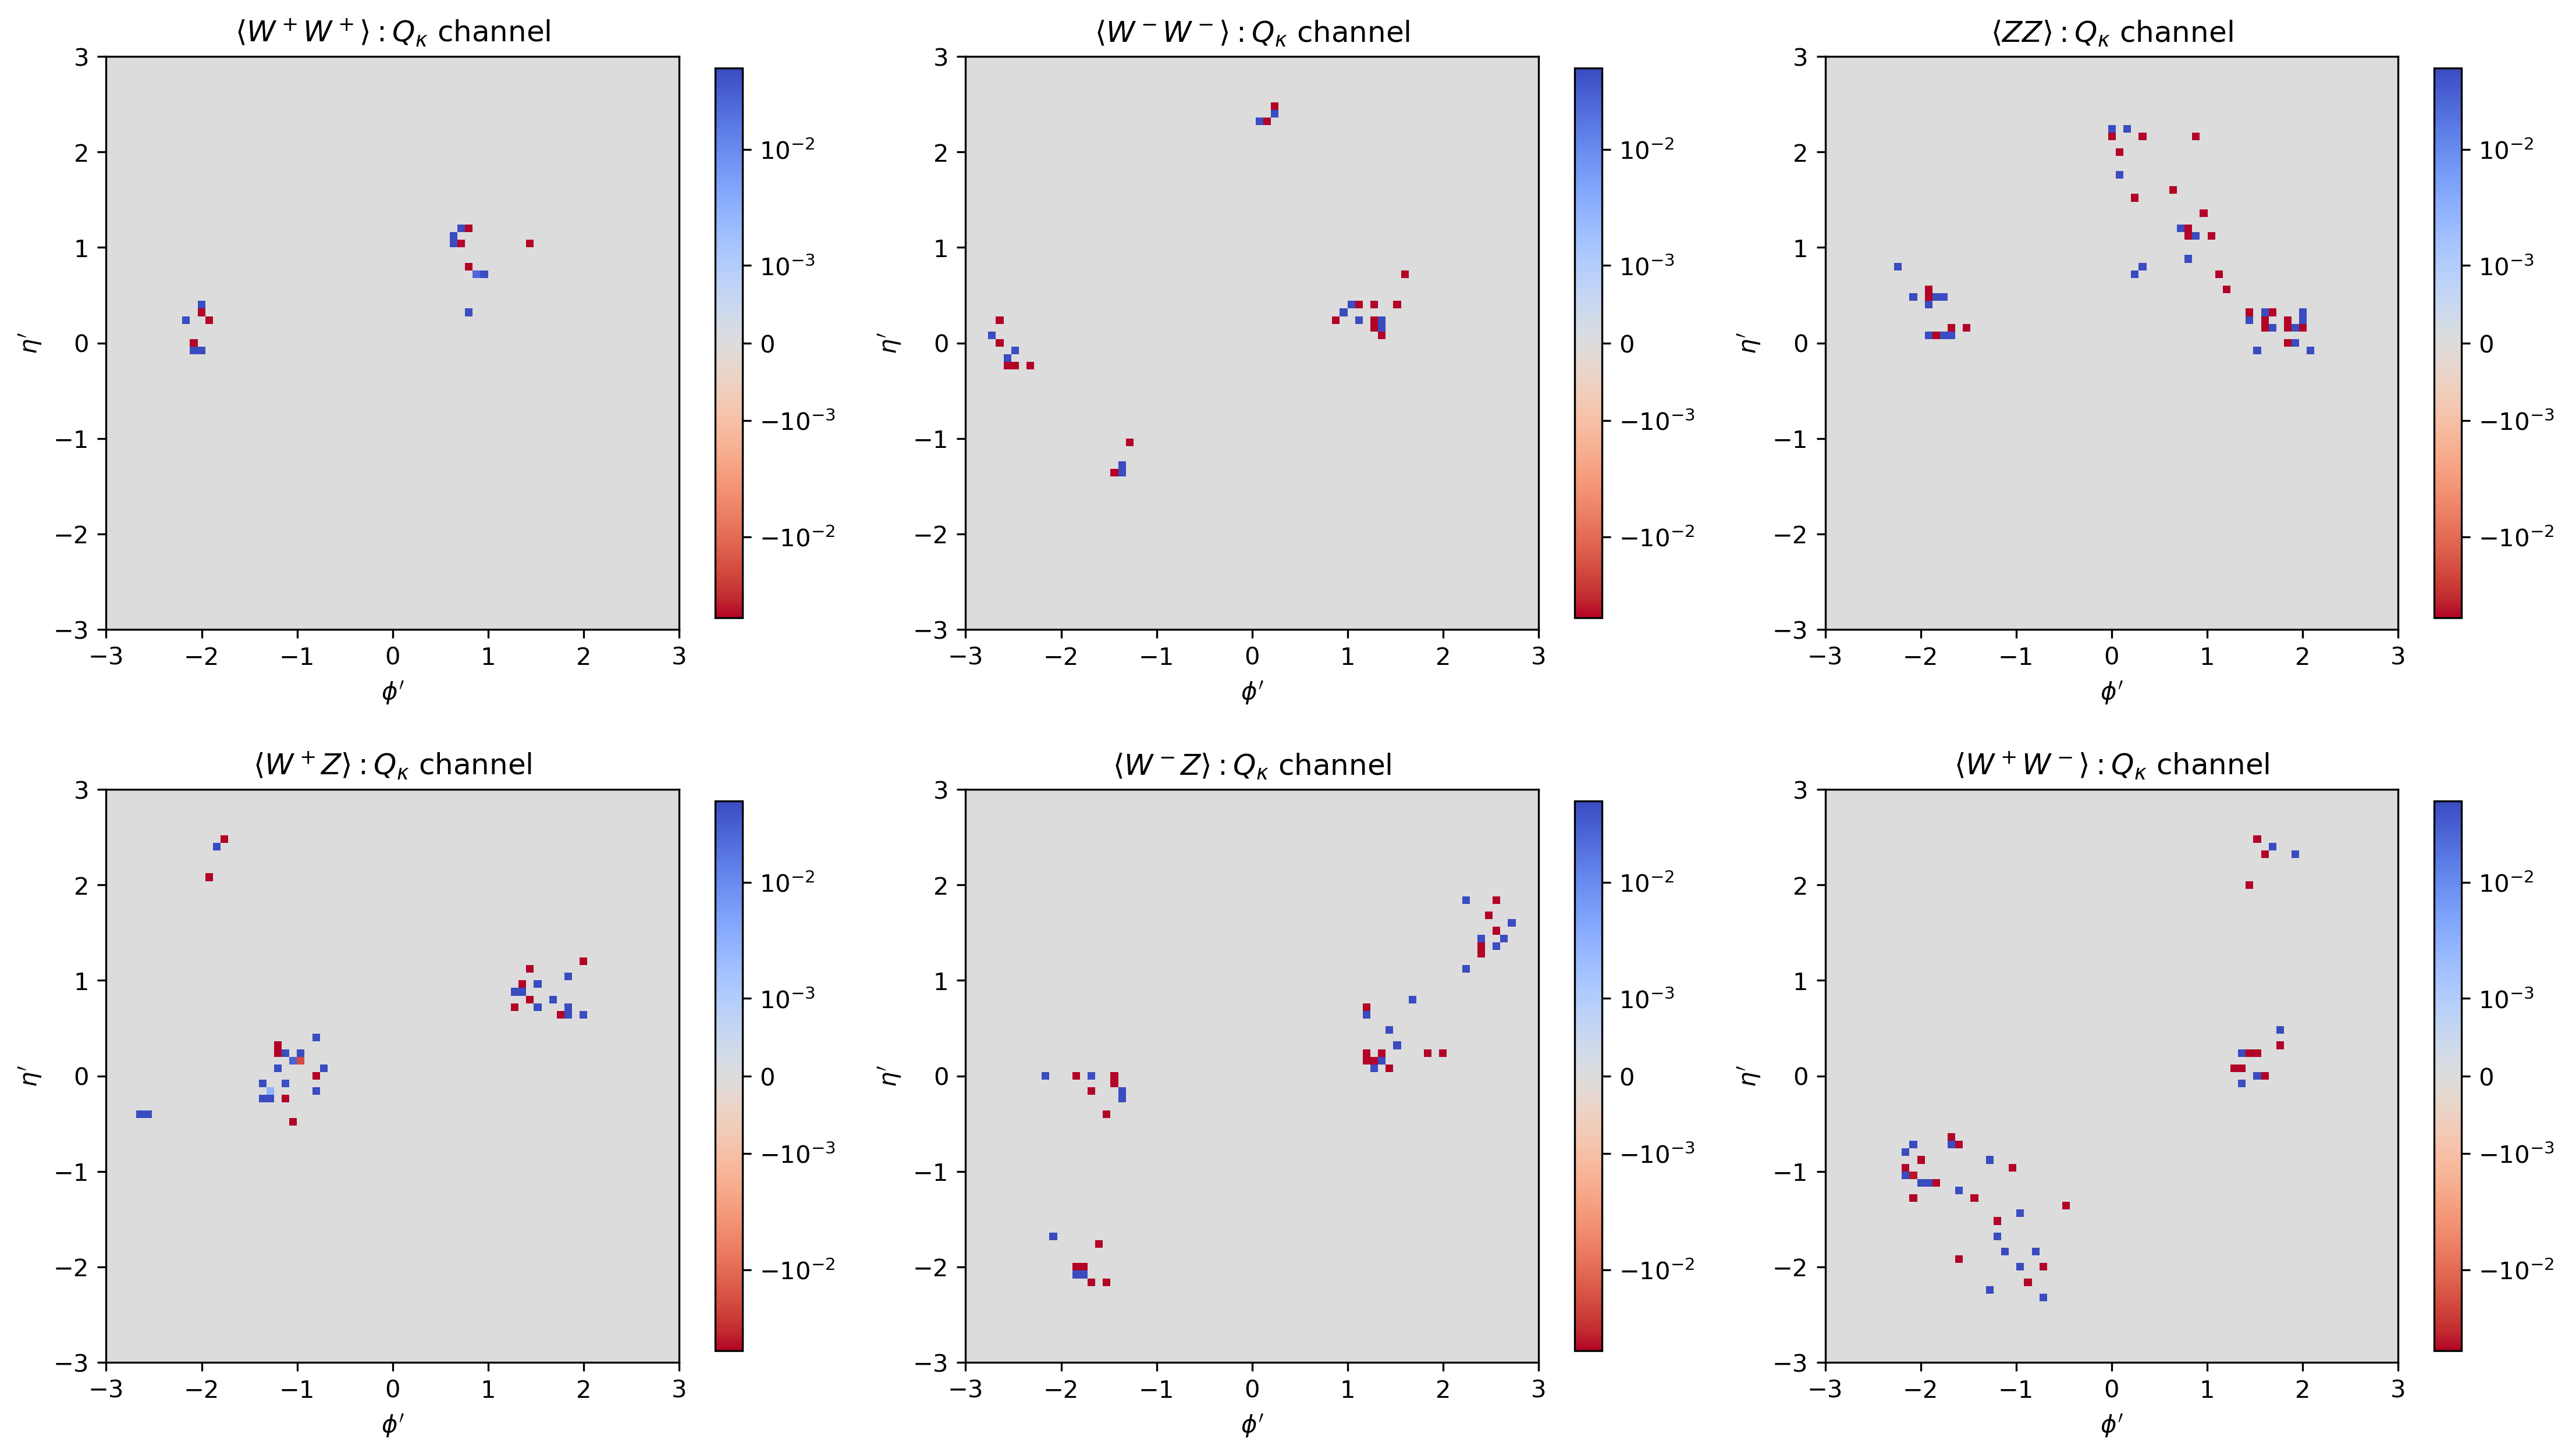
\includegraphics[width=0.95\textwidth]{single_event_image_Qk.png}
			\caption{Single event images in the $\mathcal{Q}_\kappa$ channel, with $\kappa = 0.15$.}
			\label{fig:single_event_image_Qk}
		\end{figure}
		\begin{figure}[htpb]
			\centering
			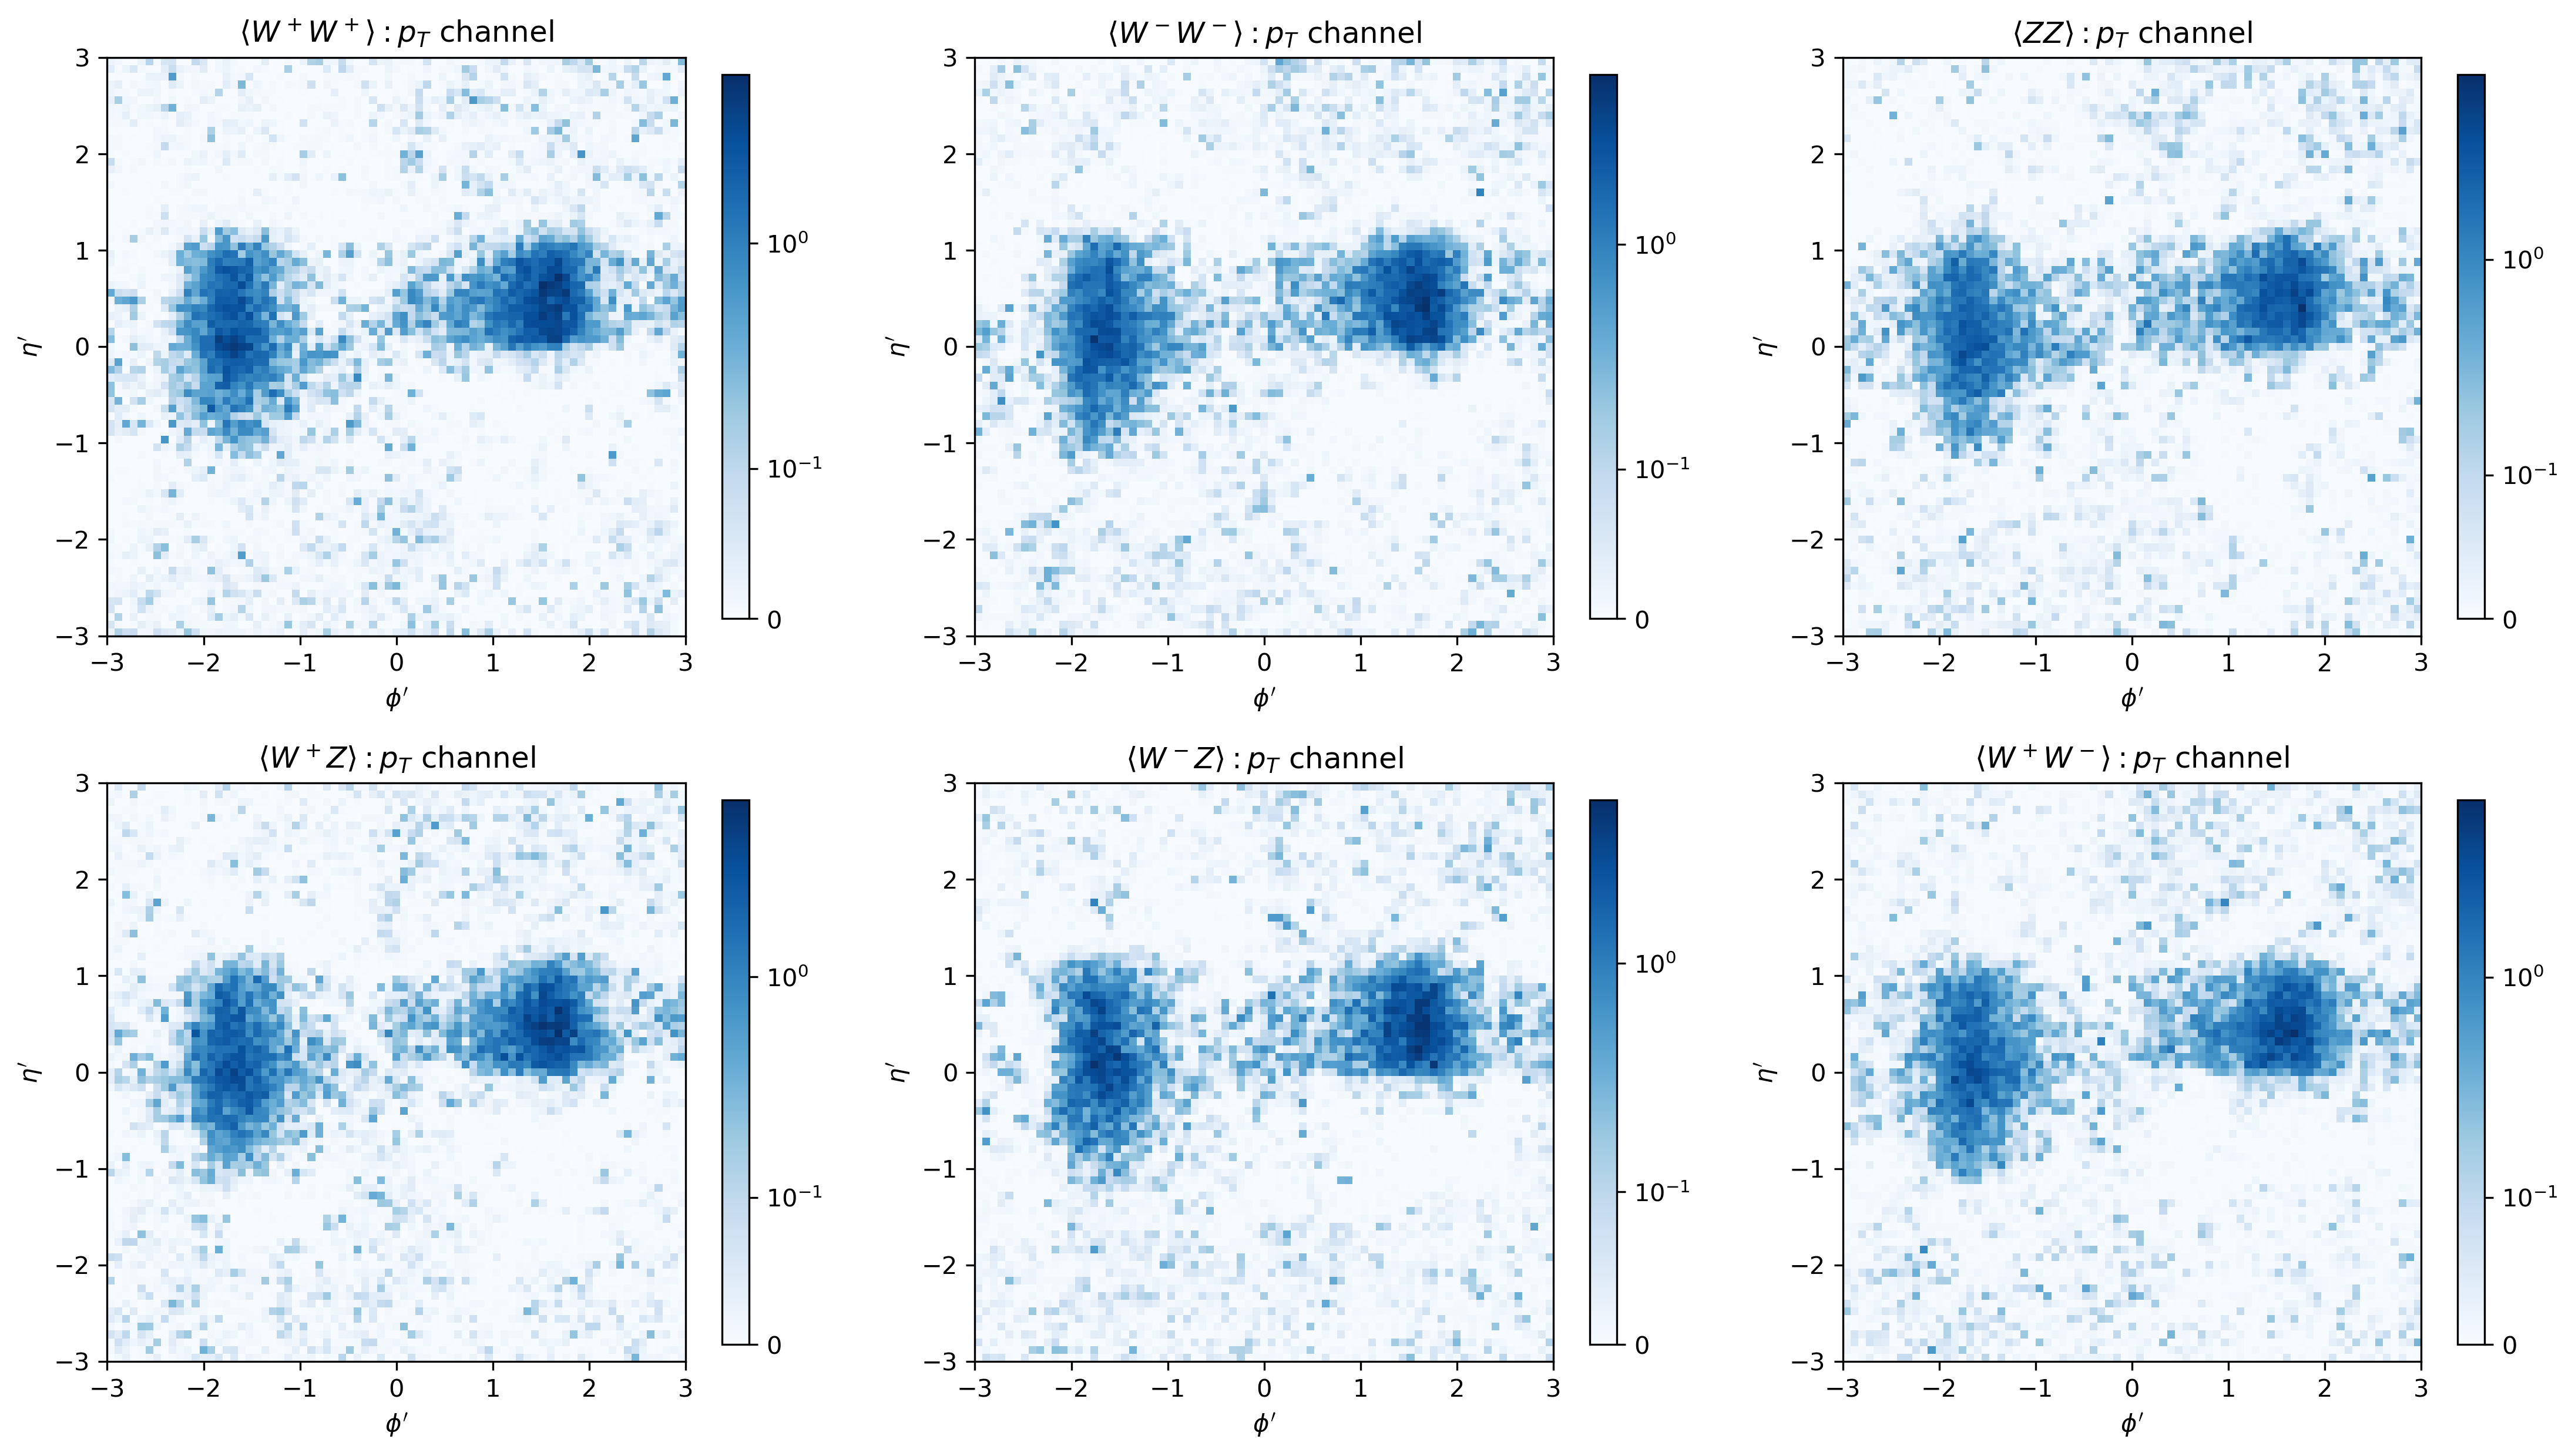
\includegraphics[width=0.95\textwidth]{event_image_PT.png}
			\caption{Average of event images in the $p_\text{T}$ channel.}
			\label{fig:event_image_PT}
		\end{figure}
		\begin{figure}[htpb]
			\centering
			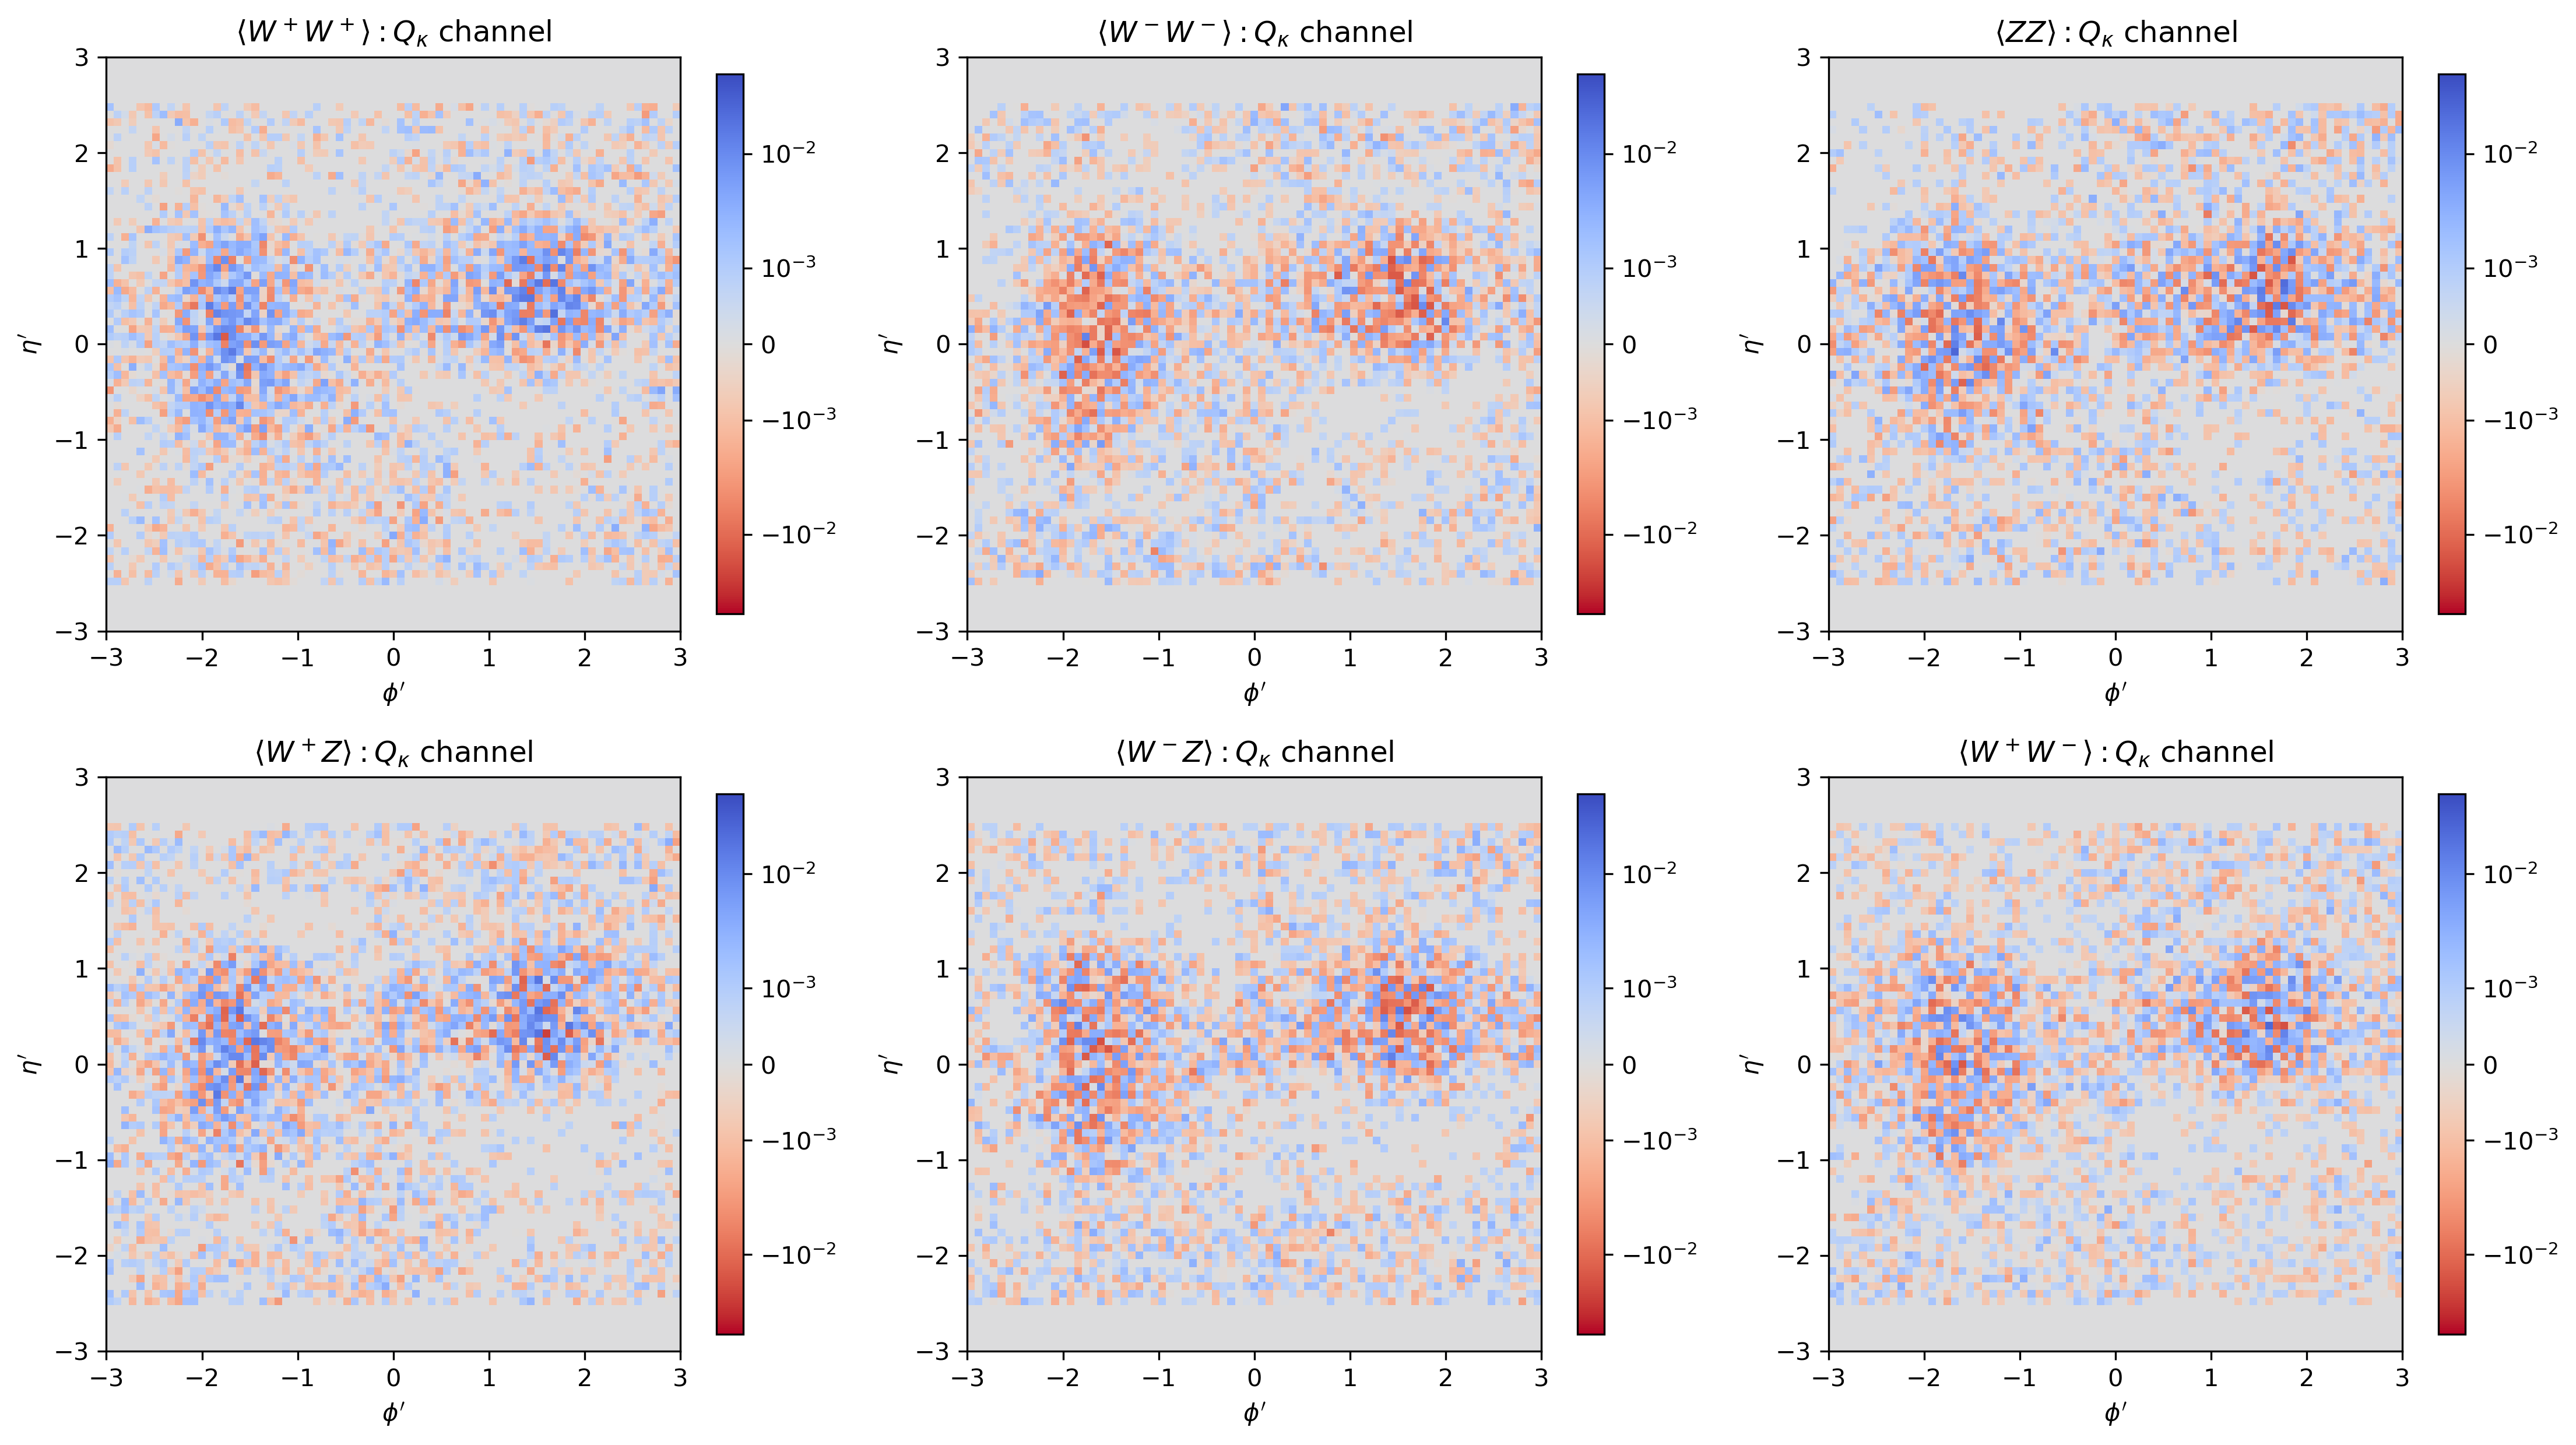
\includegraphics[width=0.95\textwidth]{event_image_Qk.png}
			\caption{Average of event images in the $\mathcal{Q}_\kappa$ channel, with $\kappa = 0.15$.}
			\label{fig:event_image_Qk}
		\end{figure}

		Figure \ref{fig:event_image_PT_ZZ-W+W+} is the $ZZ$ event image minus $W^{+}W^{+}$ event image in $p_\text{T}$ channel.
		\begin{figure}[htpb]
			\centering
			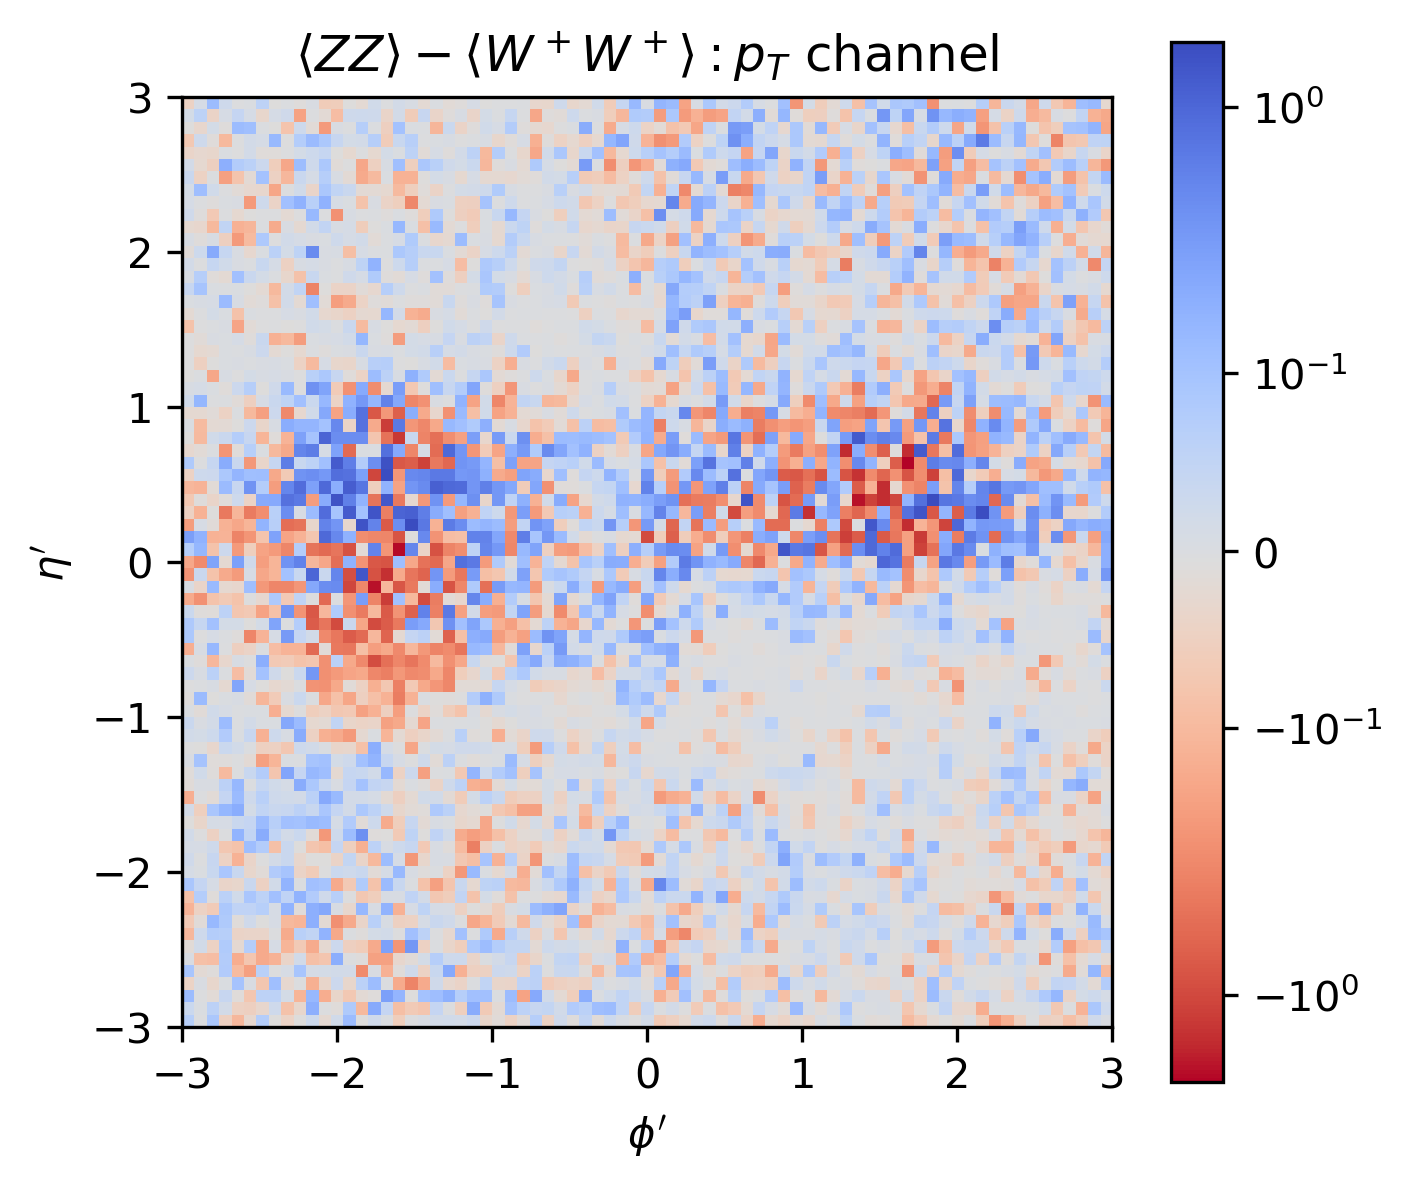
\includegraphics[width=0.5\textwidth]{event_image_PT_ZZ-W+W+.png}
			\caption{The difference between the $ZZ$ and $W^{+}W^{+}$ average event images in $p_\text{T}$ channel.}
			\label{fig:event_image_PT_ZZ-W+W+}
		\end{figure}

	% subsection event_sample_plots (end)		
% section full_event_sample (end)		
\section{Correct decay width sample}% (fold)
\label{sec:correct_decay_width_sample}
	In this section, the samples are generated with the correct decay widths, i.e., the decay width of $t, W$, and $Z$ do not change and the exotic Higgses in the GM model are set to “Auto”, meaning the decay widths are calculated by MadGraph.

	Following are the MadGraph scripts for generating $W^{+}$ sample:
	\begin{verbatim}
	import model GM_UFO
	define v = z w+ w-
	generate p p > H5pp j j $$v, (H5pp > w+ w+, (w+ > j j), (w+ > j j))
	output VBF_H5pp_ww_jjjj

	launch VBF_H5pp_ww_jjjj

	shower=Pythia8
	detector=Delphes
	analysis=OFF
	done

	set param_card tanth 2.234400e+01
	set param_card lam2 1.040100e+00
	set param_card lam3 8.829540e+00
	set param_card lam4 -2.232270e+00
	set param_card lam5 7.672600e+00
	set param_card M1coeff 1.000000e+02
	set param_card M2coeff 1.000000e+02

	set param_card wh Auto
	set param_card wh__2 Auto
	set param_card wh3p Auto
	set param_card wh3z Auto
	set param_card wh5pp Auto
	set param_card wh5p Auto
	set param_card wh5z Auto

	set run_card nevents 10000
	set run_card ebeam1 6500.0
	set run_card ebeam2 6500.0

	/home/r10222035/boosted_V_ML_test/Cards/delphes_card.dat

	done
	\end{verbatim}
	\subsection{Training results}% (fold)
	\label{sub:training_results_correct_decay_width}
		The training, validation, and testing sample size are in Table \ref{tab:sample_size_correct_decay_width}.
		\begin{table}[htpb]
			\centering
			\caption{The entries in the sum correspond to the $(W^{+}, W^{-}, Z)$ samples.}
			\label{tab:sample_size_correct_decay_width}
			\begin{tabular}{c|c|c|c}
			Case & Training set     & Validation set & Testing set   \\ \hline
			1    & $223k+232k+202k$ & $56k+57k+50k$ & $69k+72k+62k$\\
			\end{tabular}
		\end{table}

		The training results are summarized in Table \ref{tab:training_result_correct_decay_width}.
		\begin{table}[htpb]
			\centering
			\caption{The training results of correct decay width sample. The training results of CNN and CNN$^2$ are presented with an average and a standard deviation. These values are derived from 10 times training with the same dataset. Yet, the ACC value of each boson is only derived from a single result.}
			\label{tab:training_result_correct_decay_width}
			\resizebox{\textwidth}{!}{
			\begin{tabular}{c|c|c|cc|cc|cc}
										&					  &             & \multicolumn{2}{c|}{$W^{+}$} & \multicolumn{2}{c|}{$W^{-}$} & \multicolumn{2}{c}{$Z$} \\
										& Sample			  & Overall ACC & AUC        & ACC       & AUC        & ACC       & AUC       & ACC       \\ \hline
				BDT $\kappa=0.30$       &\multirow{3}{*}{1}    & 65.1 & 82.6 & 77.5 & 82.5 & 77.0 & 79.2 & 77.4\\
				CNN $\kappa=0.15$       &					   & 68.24$\pm$0.04 & 85.72$\pm$0.02 & (79.5) & 85.58$\pm$0.02 & (79.1) & 81.64$\pm$0.05 & (79.8)\\
				CNN$^2$ $\kappa=0.15$   &					   & 68.26$\pm$0.13 & 85.55$\pm$0.04 & (79.5) & 85.41$\pm$0.05 & (79.0) & 82.22$\pm$0.08 & (80.2)\\
			\end{tabular}
			}
		\end{table}
		The results are similar to the Sec.\ref{sub:cnn_results_for_modified_preprocess_and_preselection} but worse than Sec.\ref{sub:training_results}. It seems that the decay width of $t, W$, and  $Z$ will affect the training results.

		Figure \ref{fig:CNN learning curve_correct_decay_width} is CNN's loss and accuracy curve. Figure \ref{fig:CNN roc curve_correct_decay_width} is CNN's ROC.
		\begin{figure}[htpb]
			\centering
			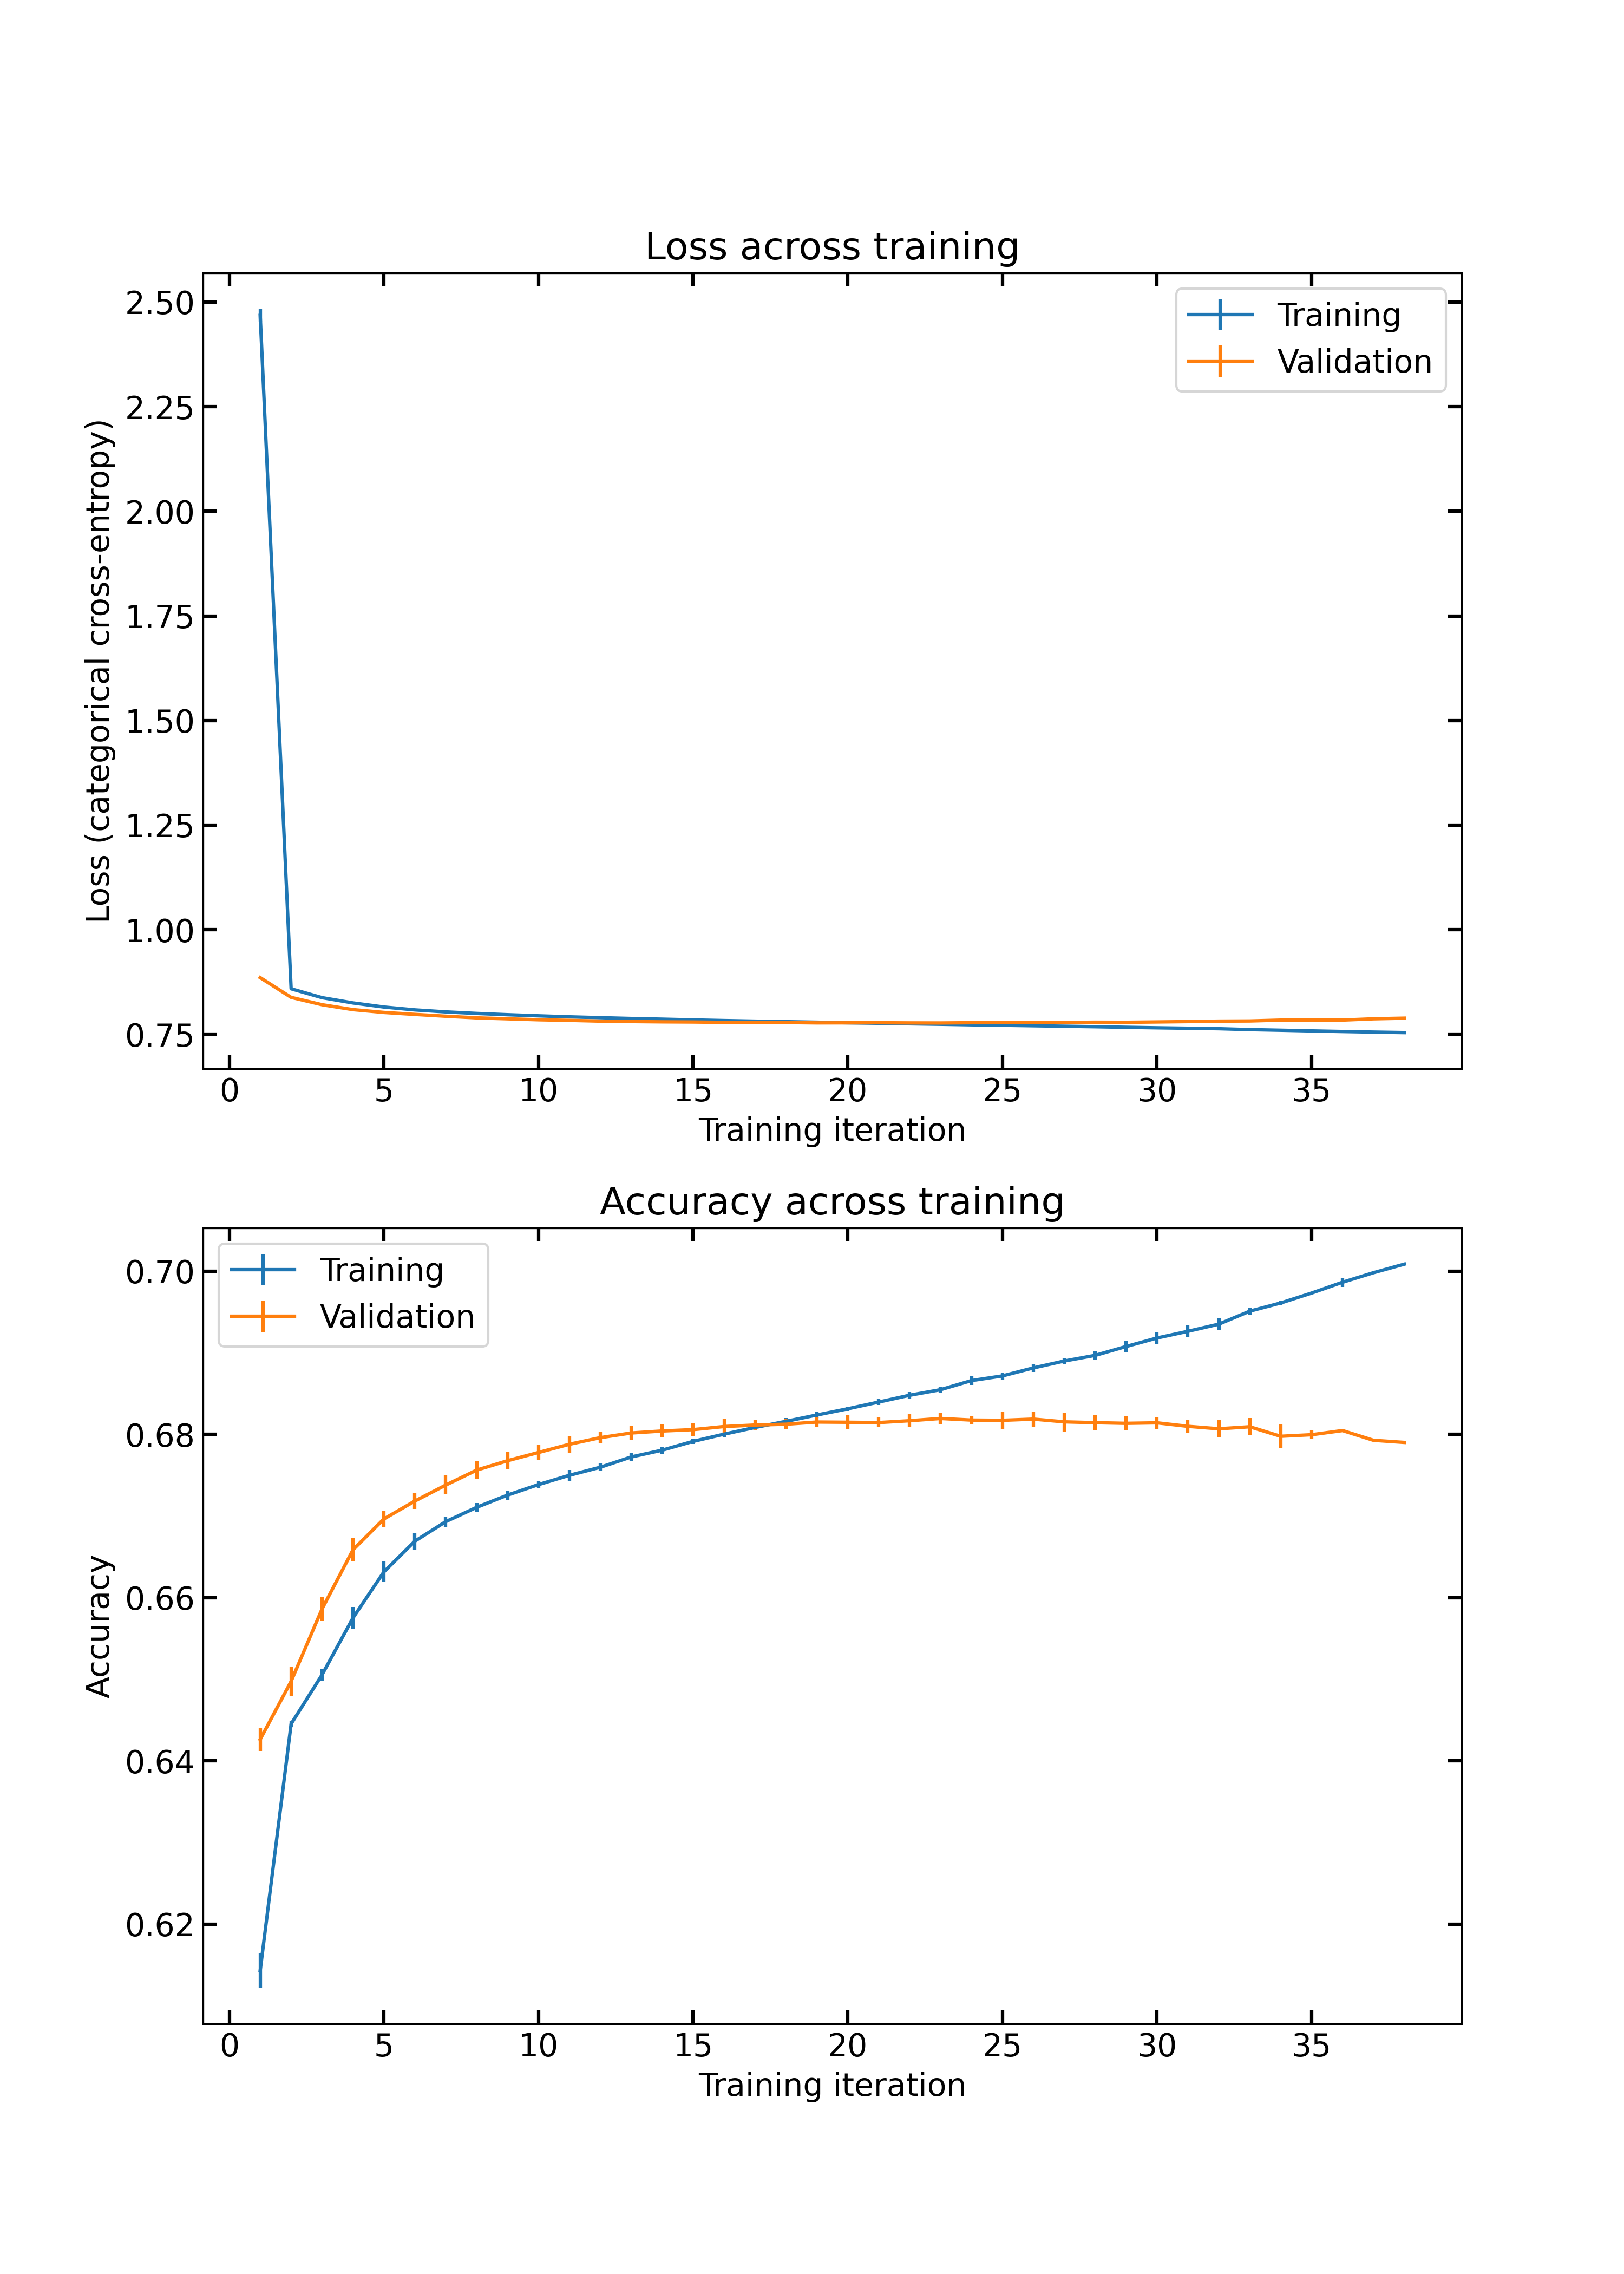
\includegraphics[width=0.90\textwidth]{CNN_loss_and_accuracy_correct_width.png}
			\caption{The loss and accuracy curve for the CNN model. Both of them are demonstrated with the average value (solid curve) and the first standard deviation range (error bar).}
			\label{fig:CNN learning curve_correct_decay_width}
		\end{figure}
		\begin{figure}[htpb]
			\centering
			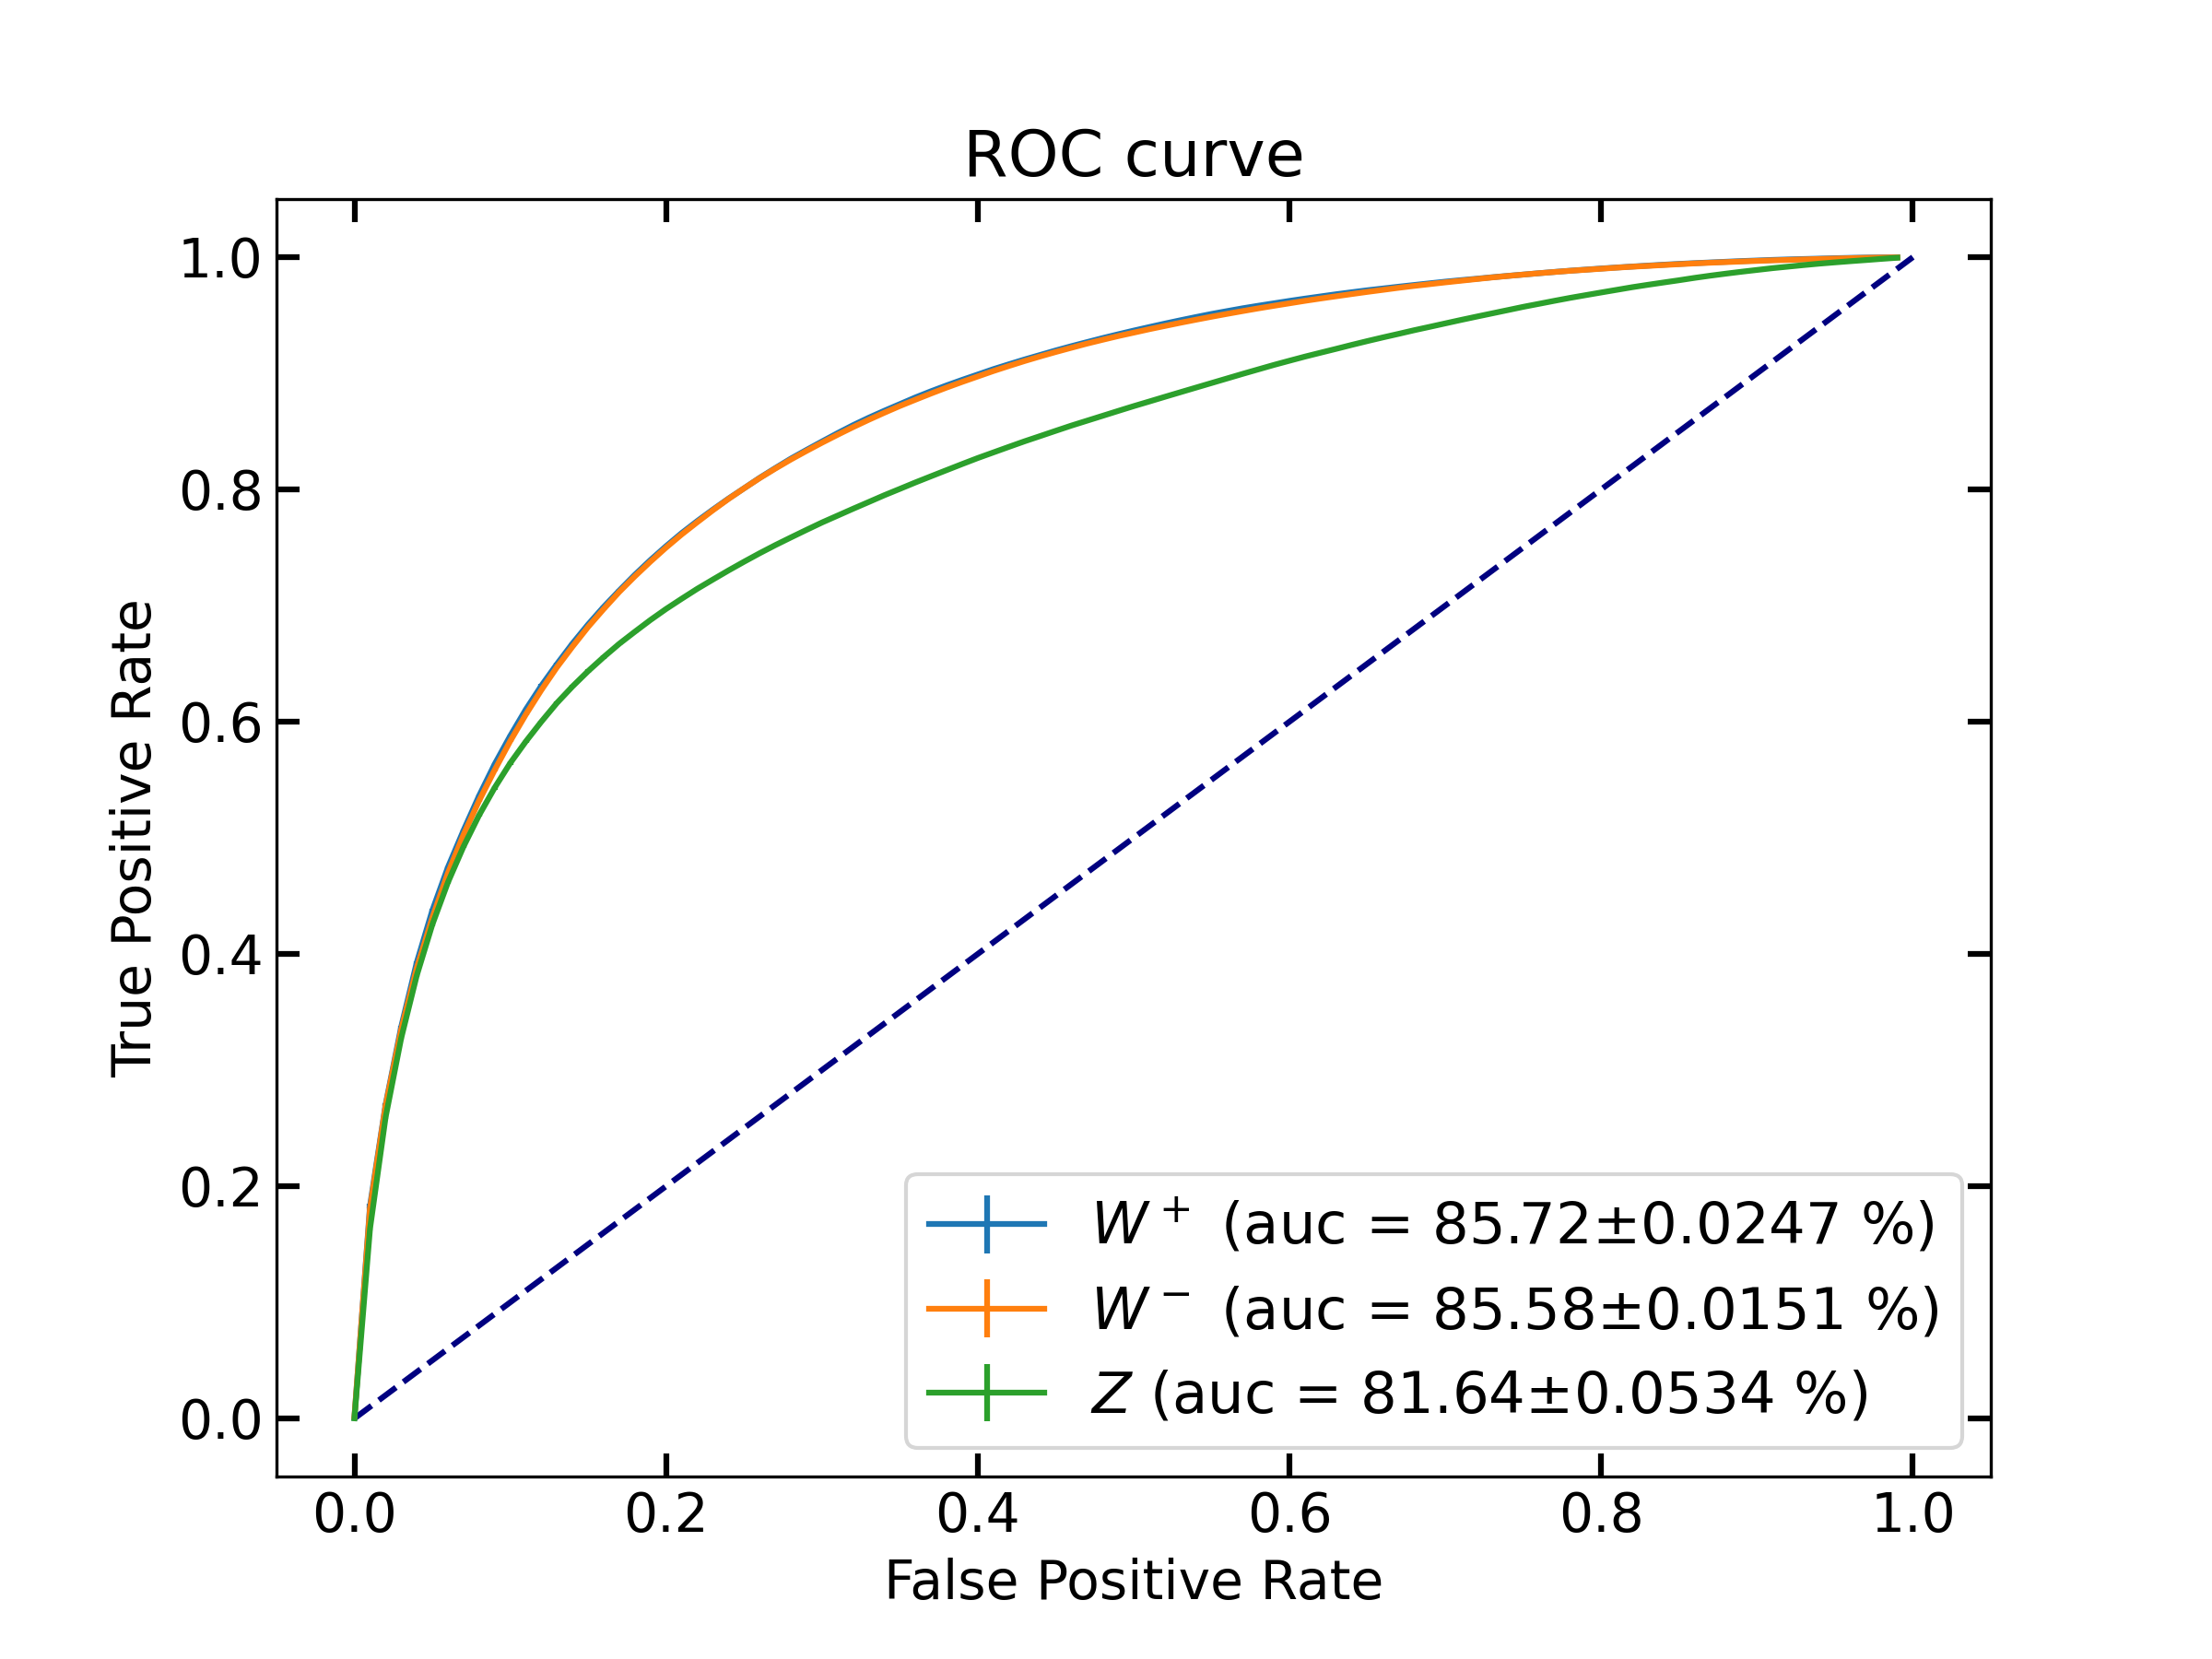
\includegraphics[width=0.70\textwidth]{CNN_roc_auc_correct_width.png}
			\caption{The ROC curve of each vector boson for the CNN model. The plotting scheme is the same as Figure \ref{fig:CNN learning curve_correct_decay_width}.}
			\label{fig:CNN roc curve_correct_decay_width}
		\end{figure}
		
		Figure \ref{fig:CNNsq learning curve_correct_decay_width} is CNN${}^2$'s loss and accuracy curve. Figure \ref{fig:CNNsq roc curve_correct_decay_width} is CNN${}^2$'s ROC.
		\begin{figure}[htpb]
			\centering
			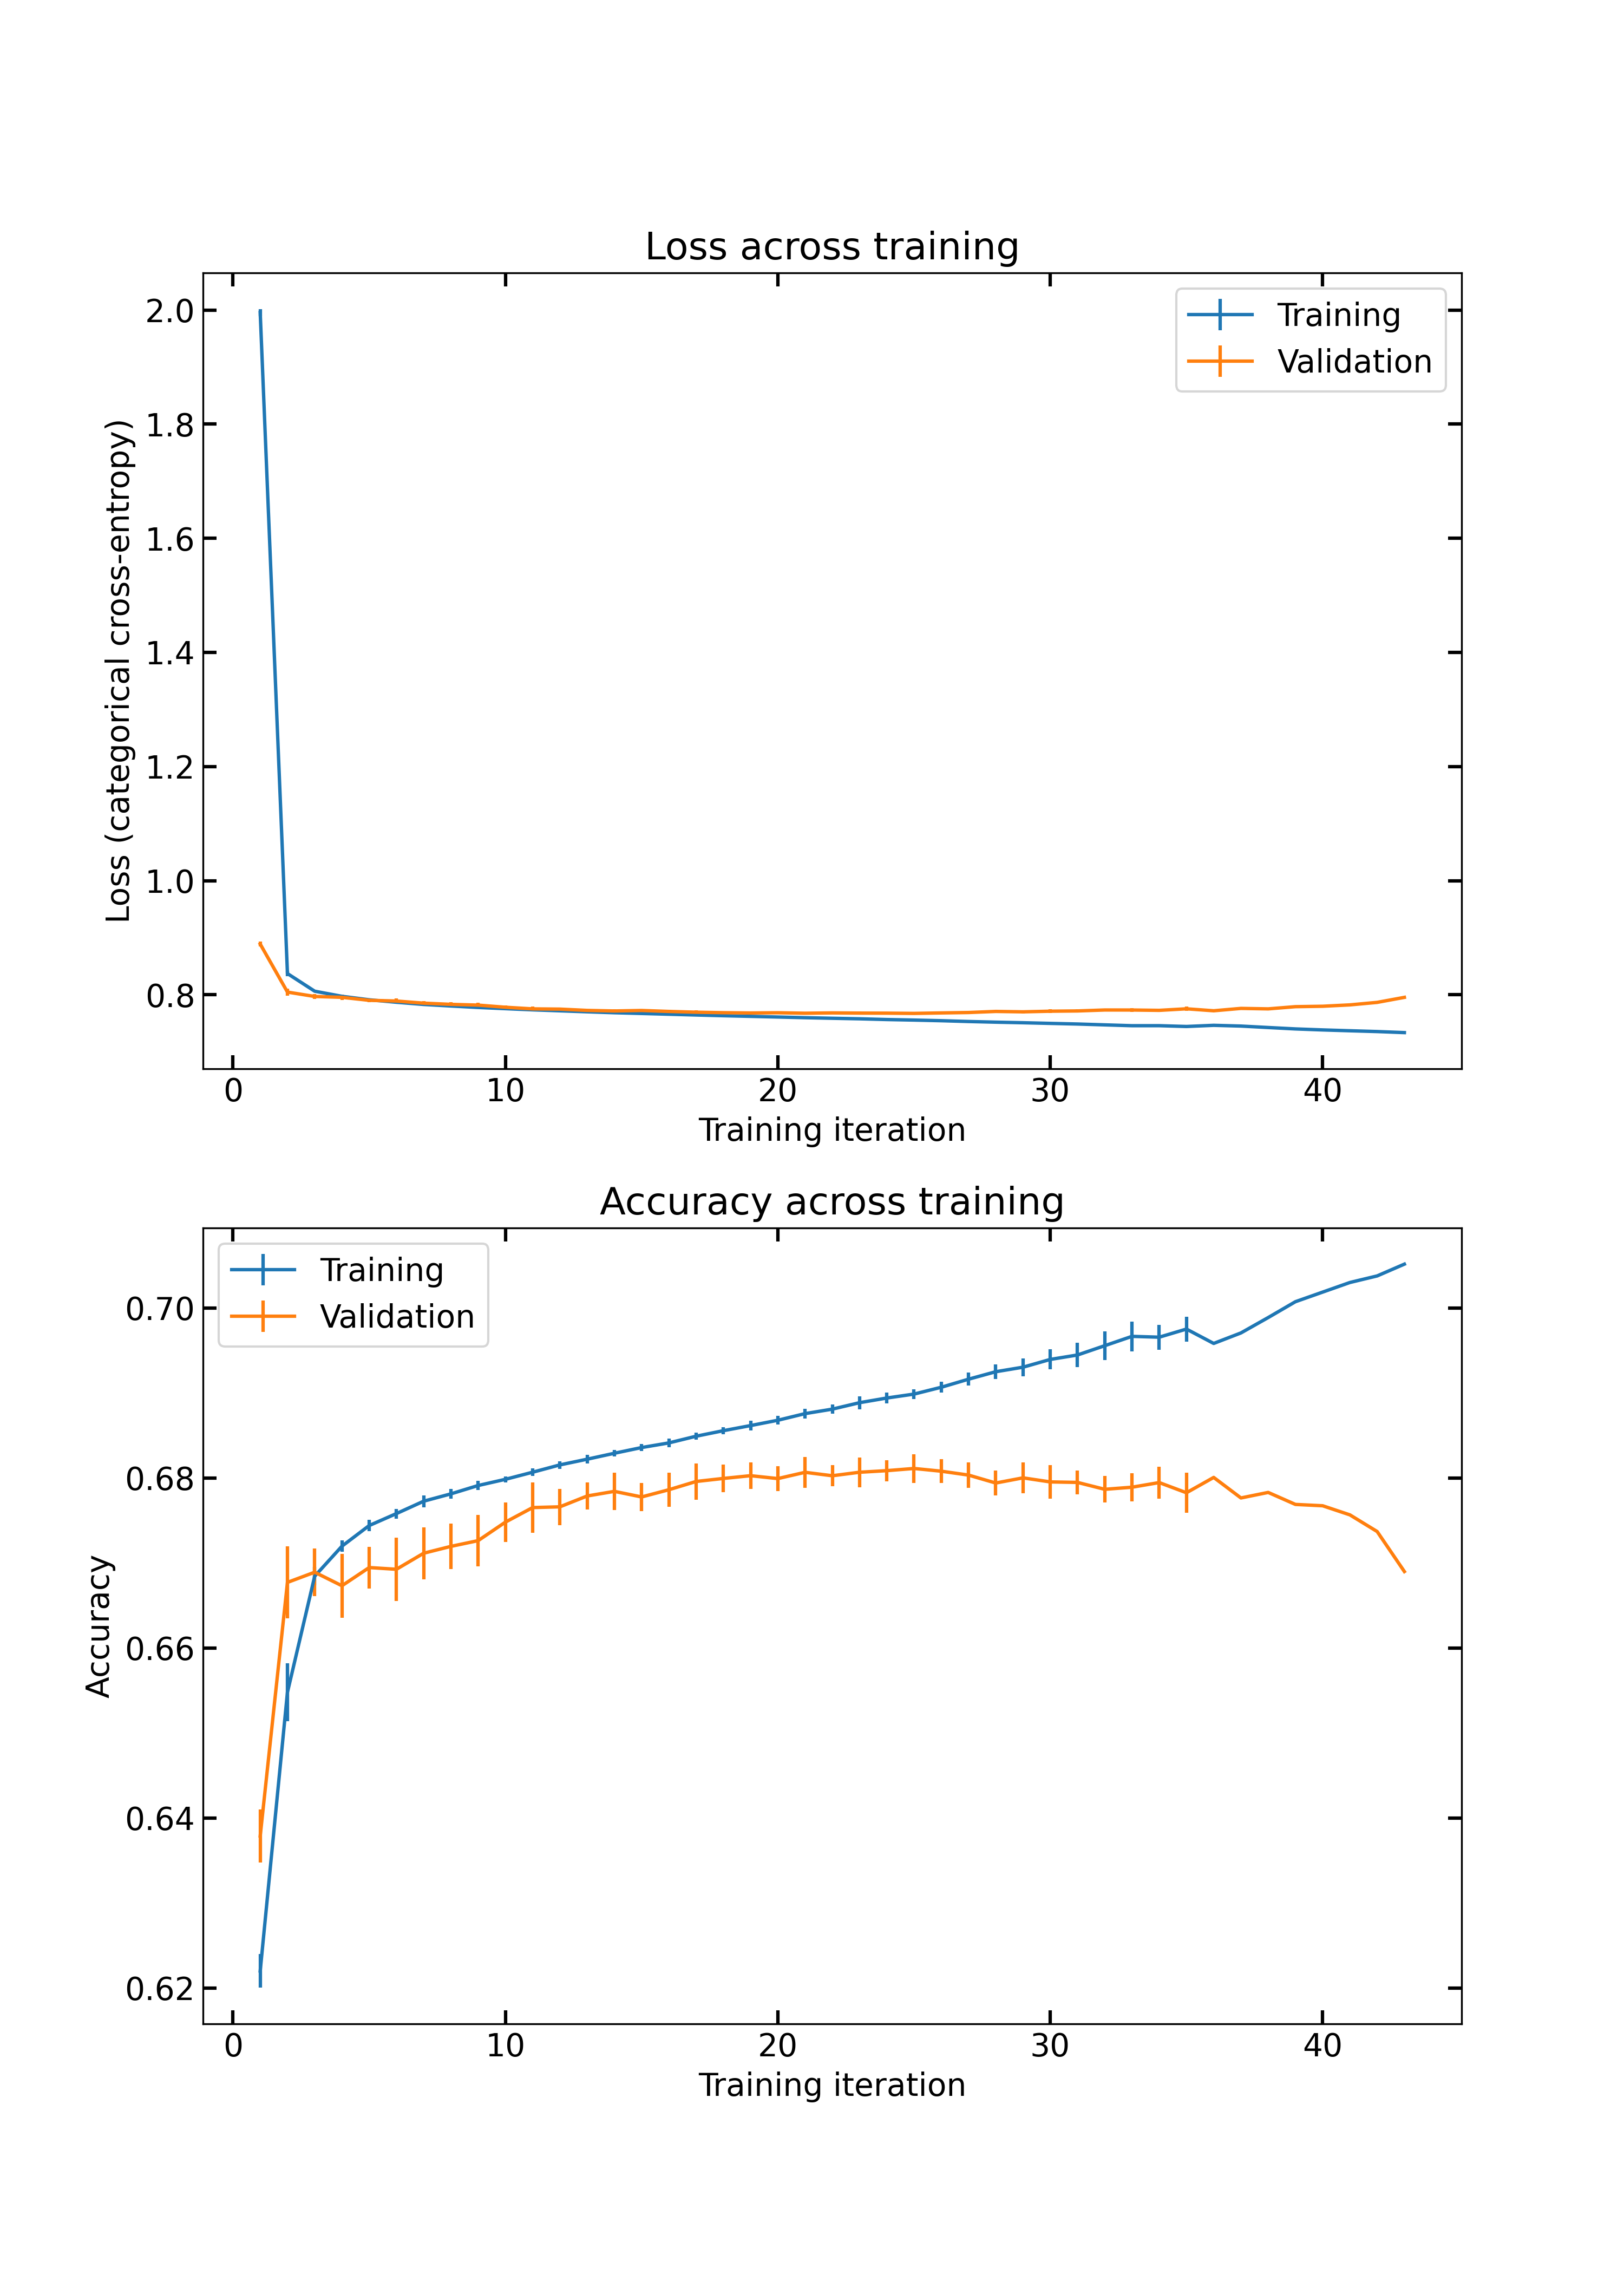
\includegraphics[width=0.90\textwidth]{CNNsq_loss_and_accuracy_correct_width.png}
			\caption{The loss and accuracy curve for the CNN$^2$ model. The plotting scheme is the same as Figure \ref{fig:CNN learning curve_correct_decay_width}.}
			\label{fig:CNNsq learning curve_correct_decay_width}
		\end{figure}
		\begin{figure}[htpb]
			\centering
			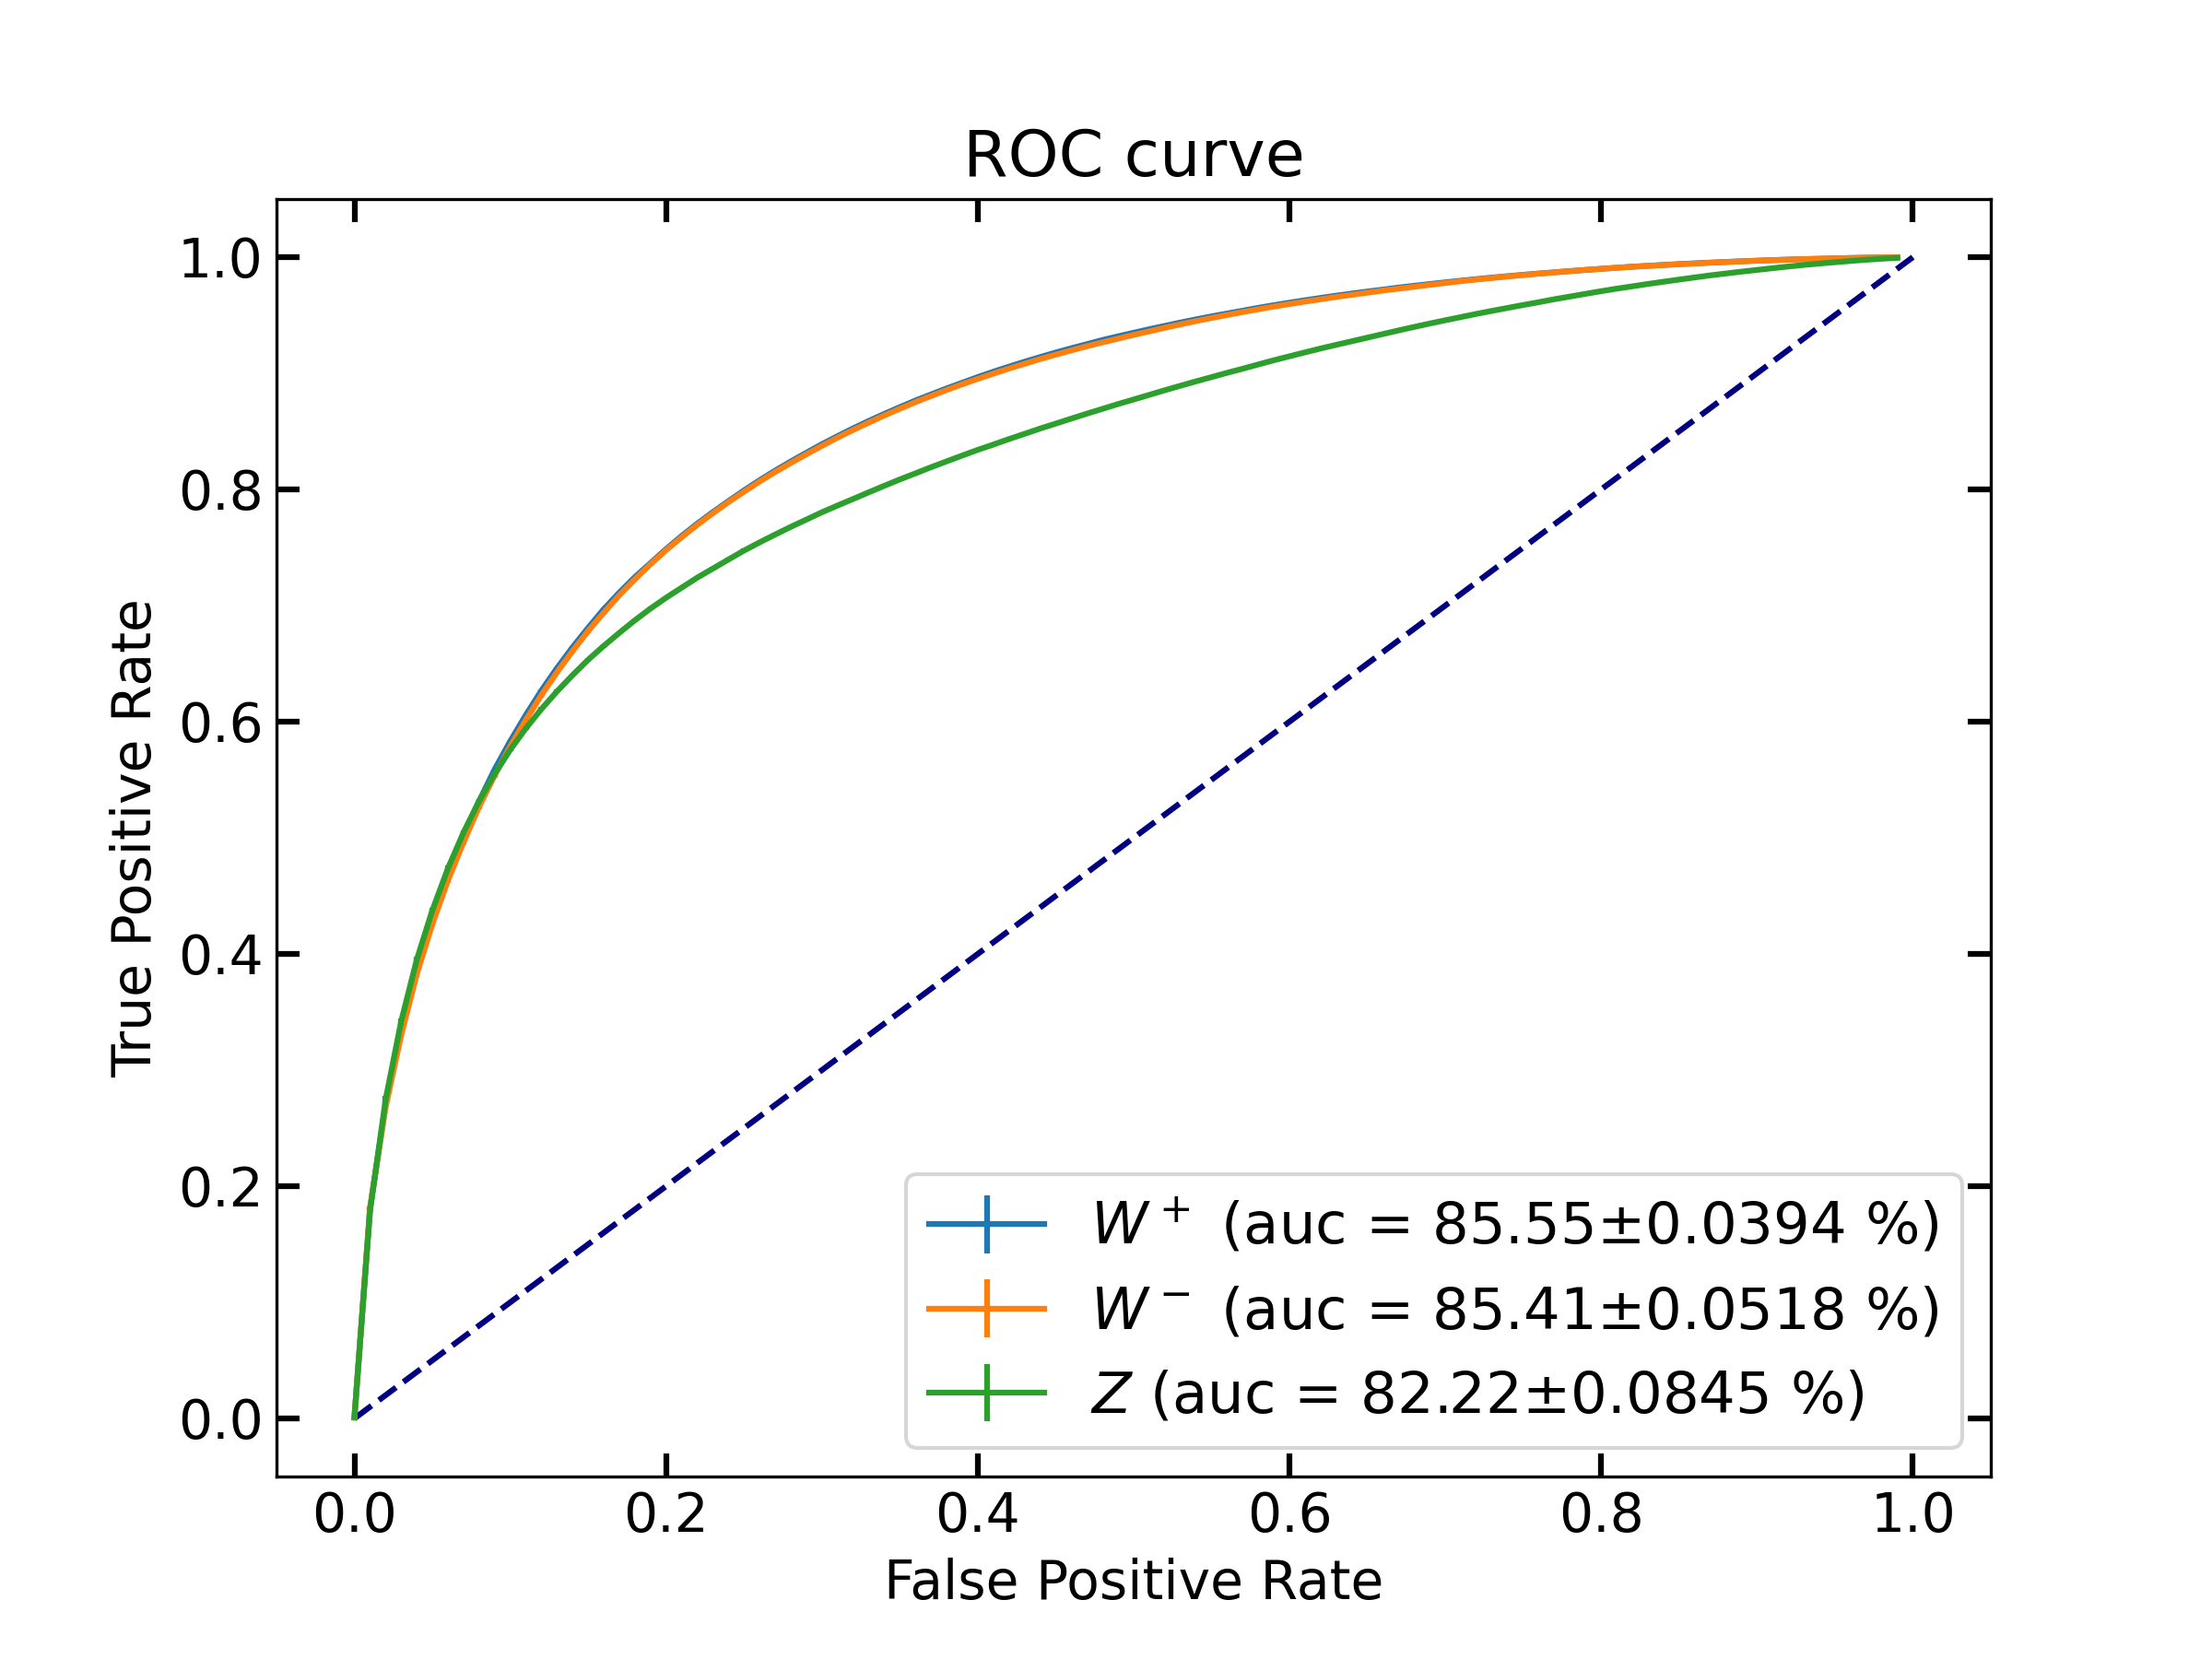
\includegraphics[width=0.70\textwidth]{CNNsq_roc_auc_correct_width.png}
			\caption{The ROC curve of each vector boson for the CNN$^2$ model. The plotting scheme is the same as Figure \ref{fig:CNN learning curve_correct_decay_width}.}
			\label{fig:CNNsq roc curve_correct_decay_width}
		\end{figure}

		\begin{figure}[htpb]
			\centering
			\subfloat[Paper]{
				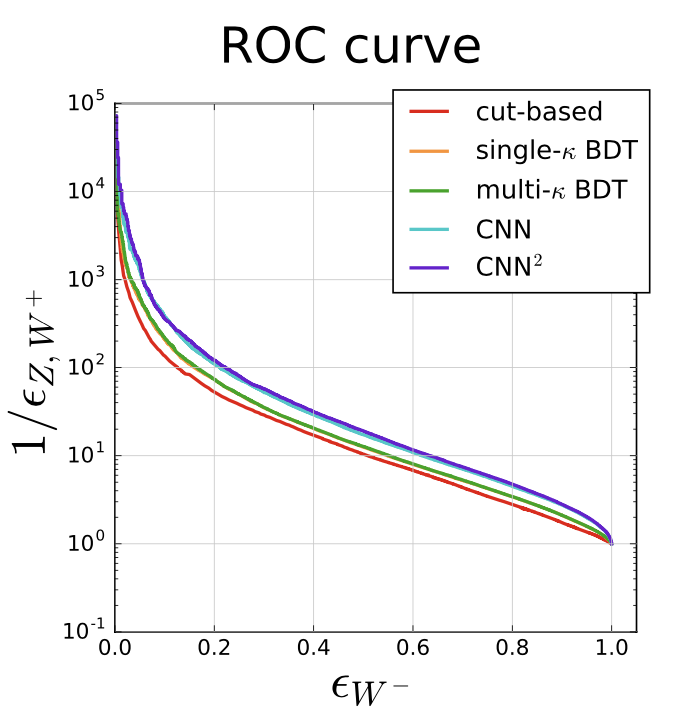
\includegraphics[width=0.4\textwidth]{ROC-paper-wm.png}
			}
			\subfloat[Ours]{
				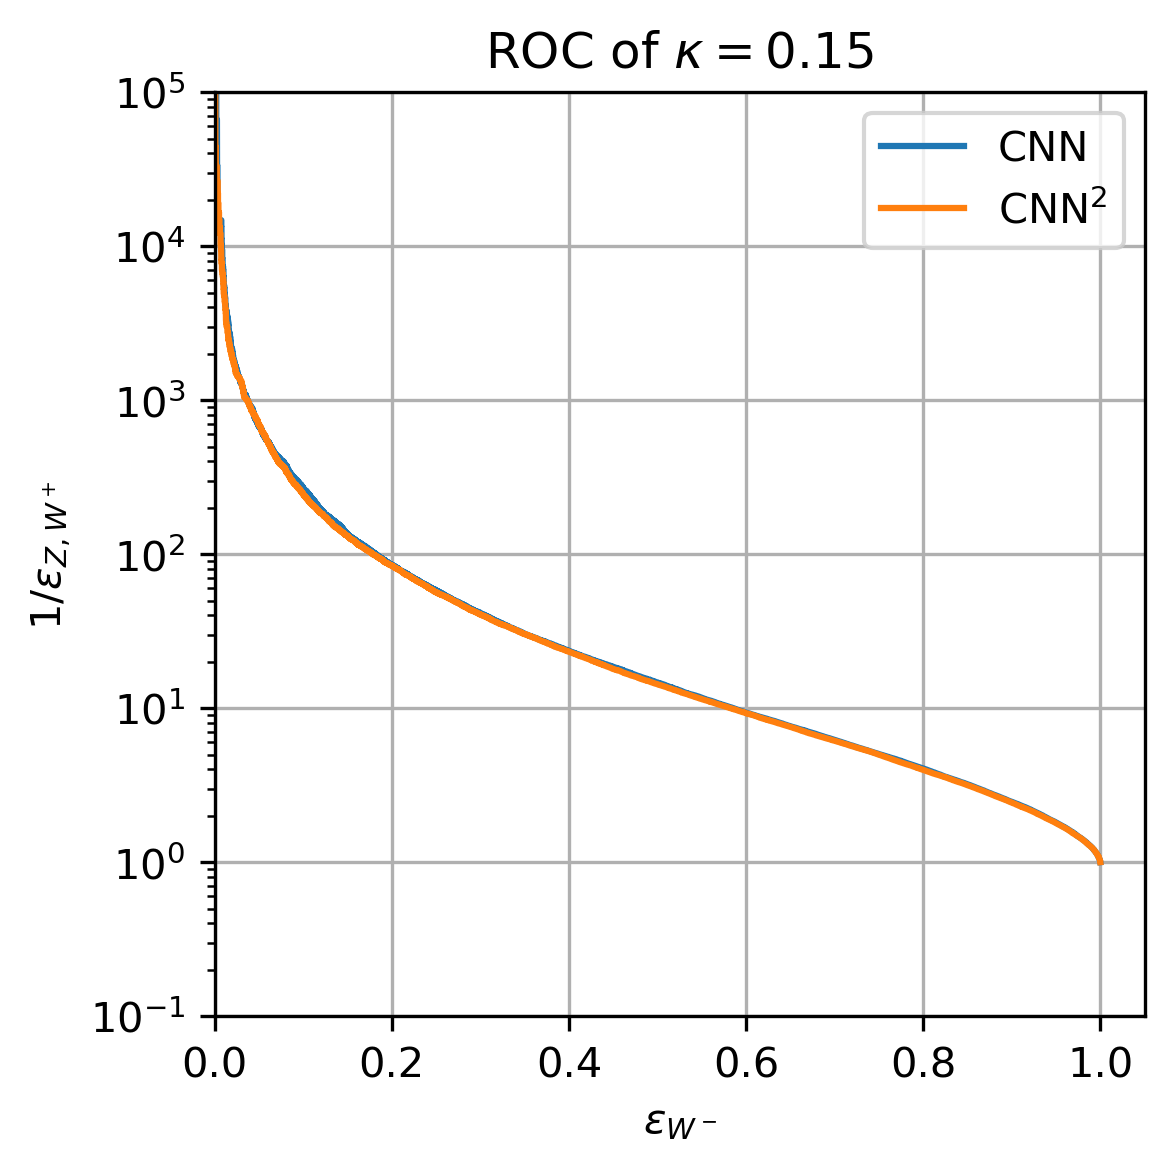
\includegraphics[width=0.4\textwidth]{ROC_kappa0.15-1000k-pstyle-wm.png}
			}
			\caption{The signal $W^{-}$ ROCs. Left is paper. Right is my result.}
			\label{fig:ROCs_wm}
		\end{figure}
		\begin{figure}[htpb]
			\centering
			\subfloat[Paper]{
				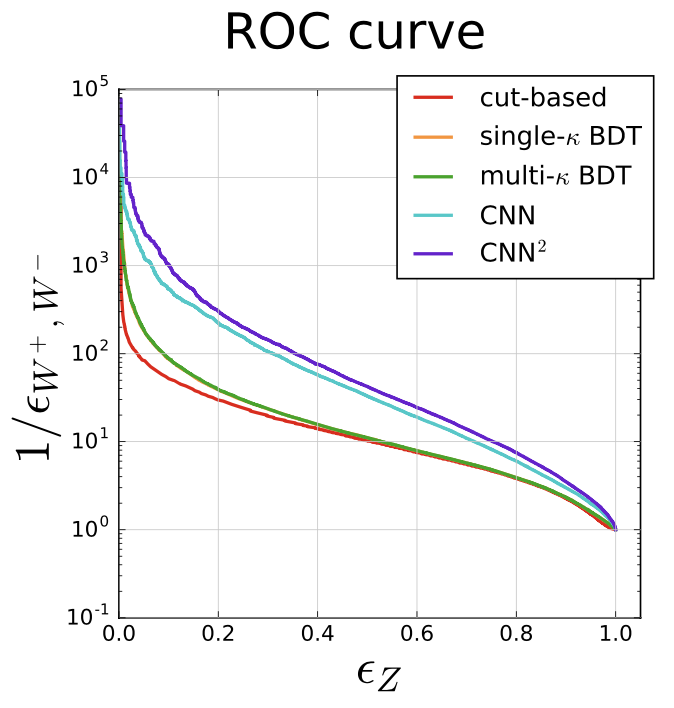
\includegraphics[width=0.4\textwidth]{ROC-paper-z.png}
			}
			\subfloat[Ours]{
				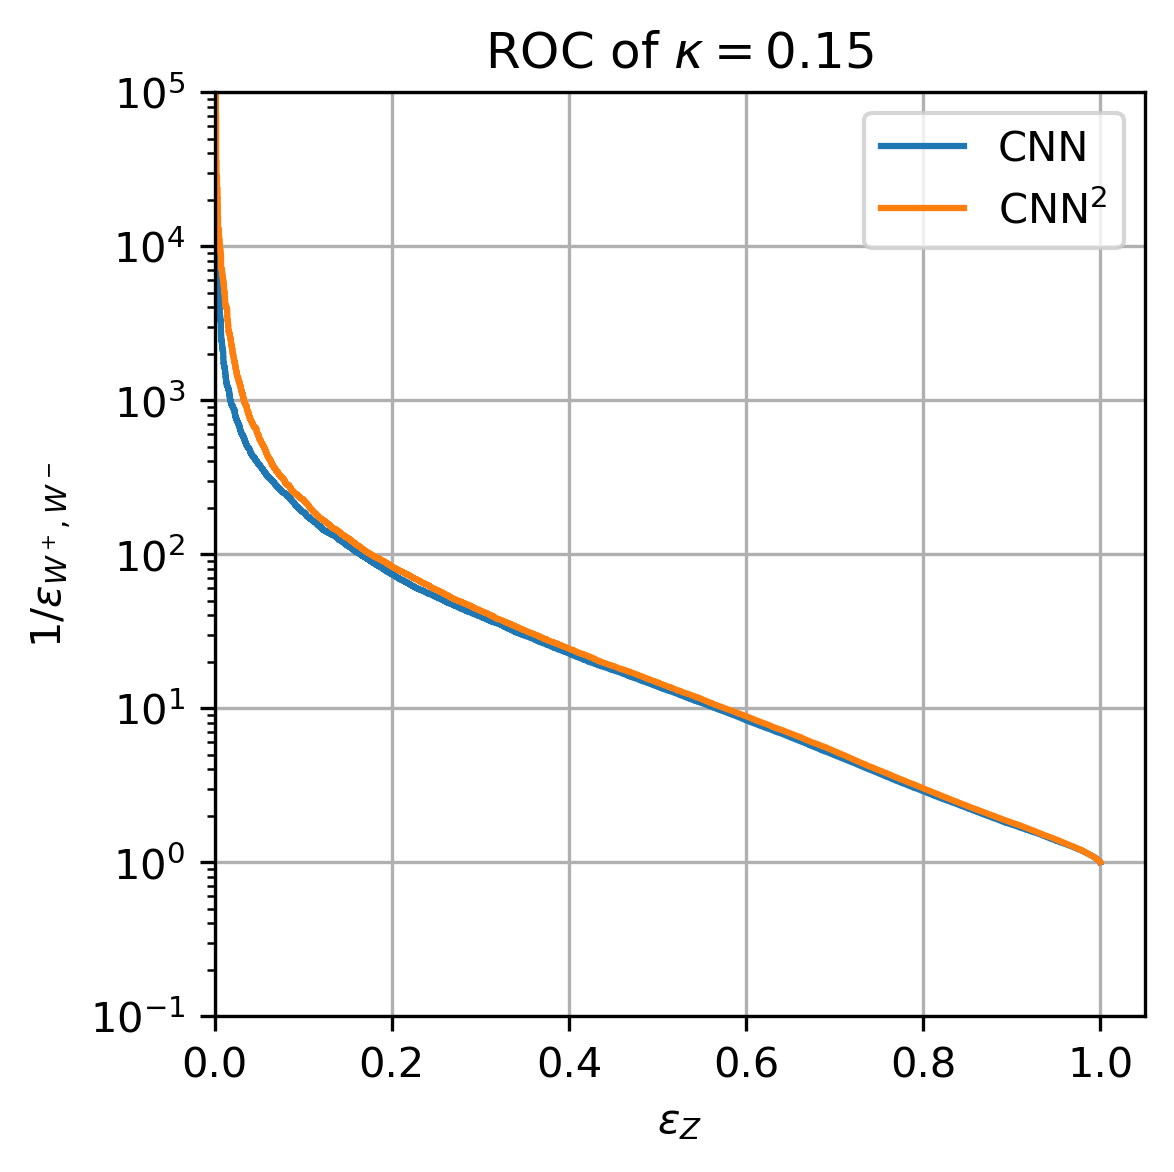
\includegraphics[width=0.4\textwidth]{ROC_kappa0.15-1000k-pstyle-z.png}
			}
			\caption{The signal $Z$ ROCs. Left is paper. Right is my result.}
			\label{fig:ROCs_z}
		\end{figure}

		\begin{figure}[htpb]
			\centering
			\subfloat[CNN]{
				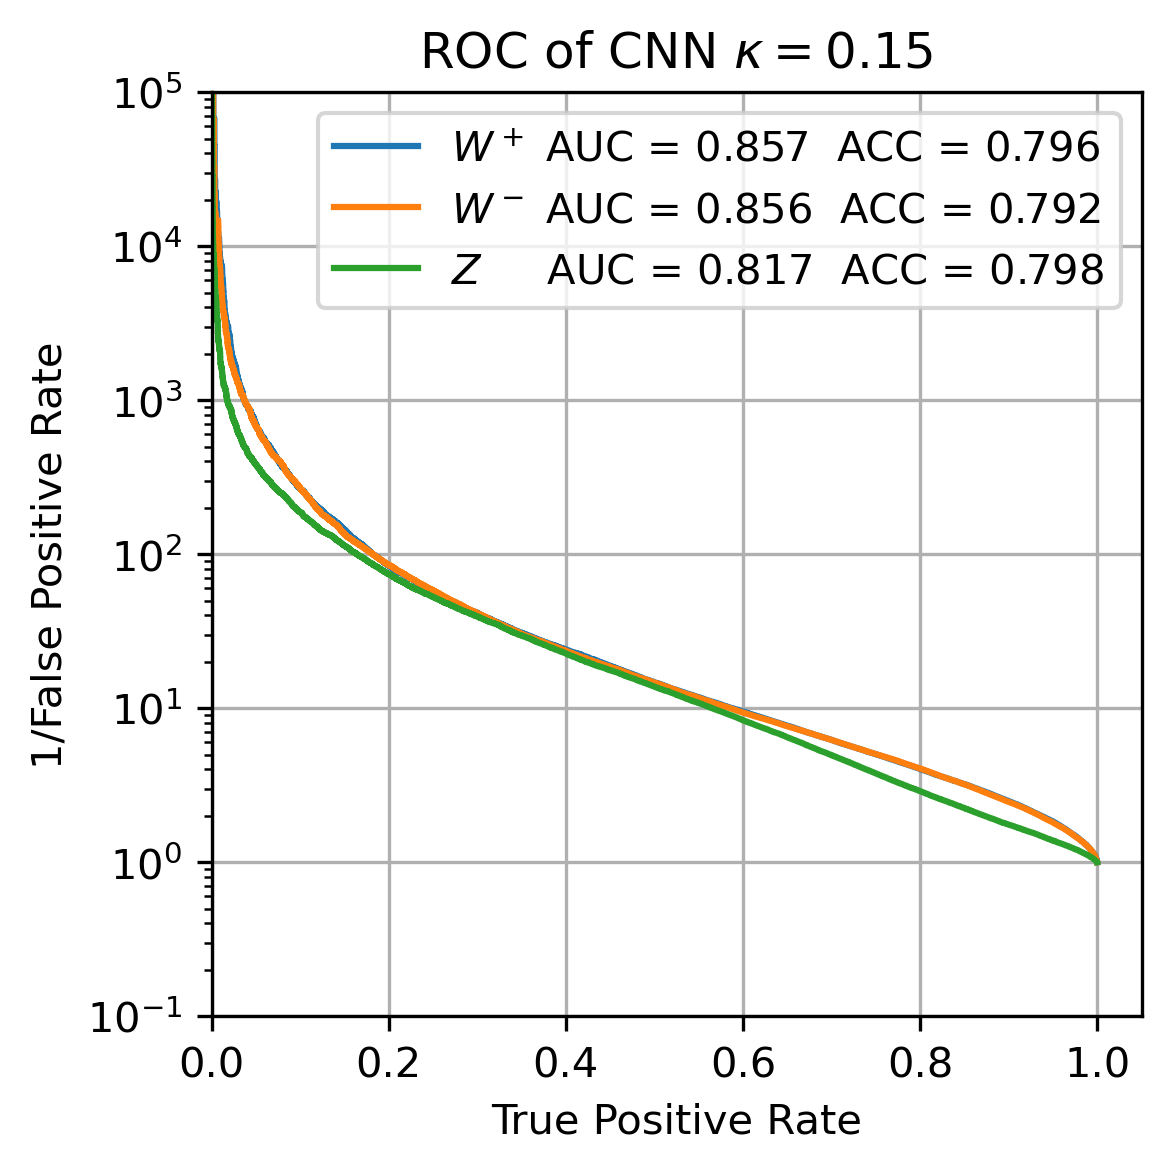
\includegraphics[width=0.4\textwidth]{ROC_CNN_kappa0.15-1000k-pstyle.png}
			}
			\subfloat[CNN${}^2$]{
				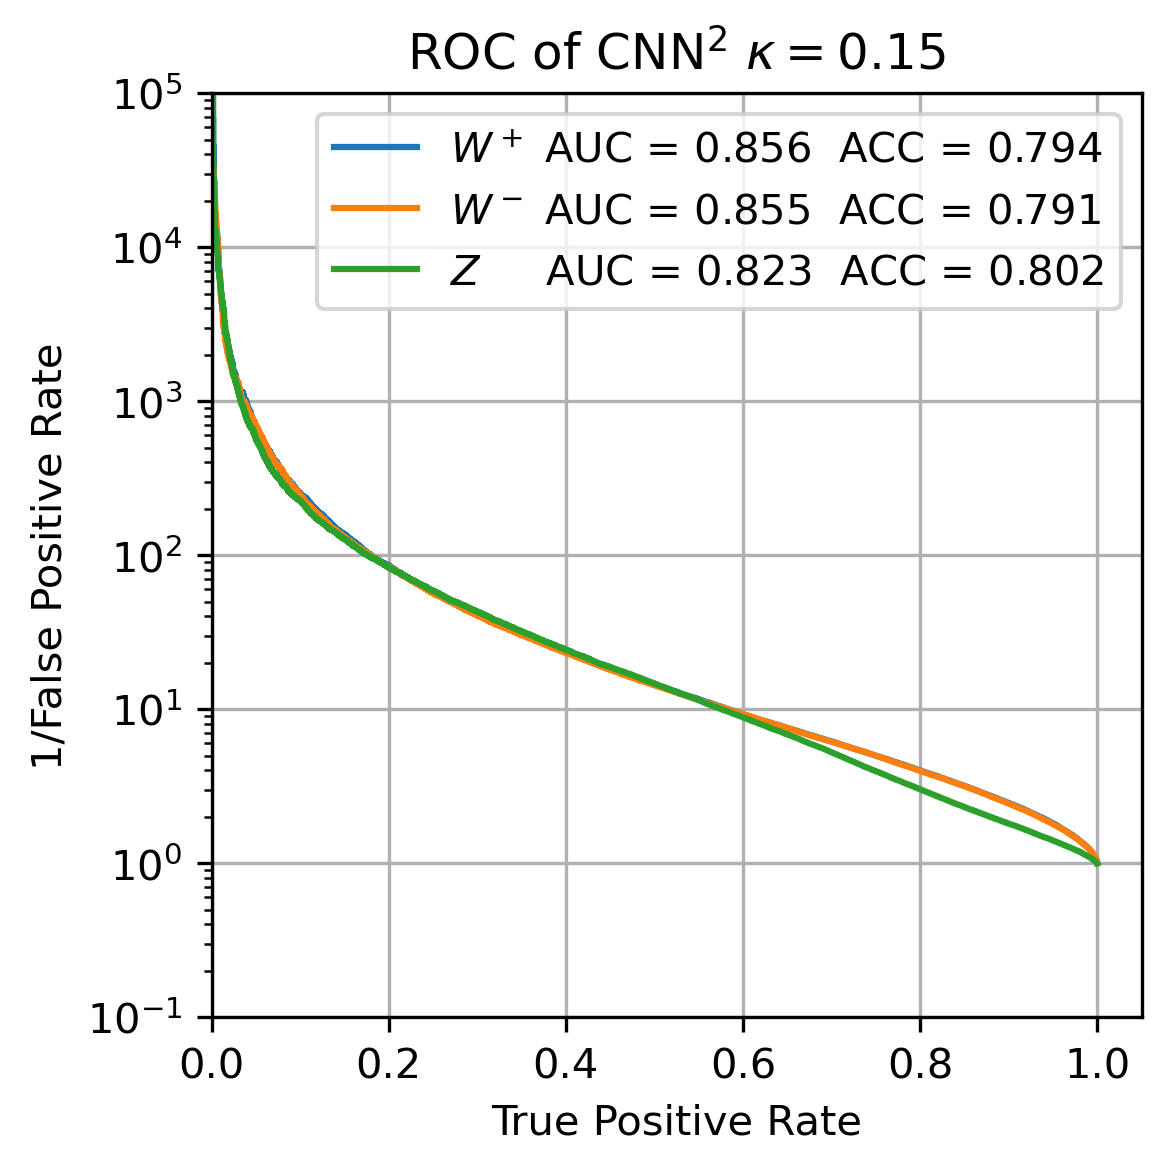
\includegraphics[width=0.4\textwidth]{ROC_CNNsq_kappa0.15-1000k-pstyle.png}
			}
			\caption{The ROCs of my training results. For the left one, the model is CNN. For right one, the model is CNN${}^{2}$.}
			\label{fig:ROCs_my}
		\end{figure}

	% subsection training_results (end)
% section correct_decay_width_sample (end)		
\section{Full event training}% (fold)
\label{sec:full_event_training}
	\subsection{Training sample size}% (fold)
	\label{sub:full_event_training_sample_size}
		The event sample size for each type is presented in Table \ref{tab:full_event_sample_size}
		\begin{table}[htpb]
			\centering
			\caption{The sample size for each type. 80\% samples are used in training, and 20\% samples are used in testing.}
			\label{tab:full_event_sample_size}
			\begin{tabular}{c|c|c|c|c|c|c|c}
			Case &$\kappa$& $W^+W^+$ & $W^-W^-$ & $ZZ$ & $W^+Z$ & $W^-Z$ & $W^+W^-$ \\ \hline
			1    & 0.15   & 47k      & 51k      & 38k  & 42k    & 44k    & 48k     
			\end{tabular}
		\end{table}
	% subsection full_event_training_sample_size (end)
	\subsection{Training results}% (fold)
	\label{sub:full_event_training_results}
		The training results are summarized in Table \ref{tab:training_result_event}.
		\begin{table}[htpb]
			\centering
			\caption{The training results of the full event.}
			\label{tab:training_result_event}
			\resizebox{\textwidth}{!}{
			\begin{tabular}{c|c|c|cc|cc|cc|cc|cc|cc}
										 &                    & Overall & \multicolumn{2}{c}{$W^+W^+$} & \multicolumn{2}{c}{$W^-W^-$} & \multicolumn{2}{c}{$ZZ$} & \multicolumn{2}{c}{$W^+Z$} & \multicolumn{2}{c}{$W^-Z$} & \multicolumn{2}{c}{$W^+W^-$} \\
					  & Sample             & ACC   & AUC   & ACC   & AUC   & ACC   & AUC   & ACC   & AUC   & ACC   & AUC   & ACC   & AUC   & ACC   \\ \hline
			CNN       & \multirow{2}{*}{1} & 0.451 & 0.860 & 0.858 & 0.855 & 0.850 & 0.797 & 0.868 & 0.740 & 0.845 & 0.737 & 0.842 & 0.741 & 0.830 \\
			CNN${}^2$ &                    & 0.379 & 0.830 & 0.846 & 0.822 & 0.837 & 0.684 & 0.858 & 0.687 & 0.842 & 0.686 & 0.840 & 0.690 & 0.826
			\end{tabular}			
			}
		\end{table}

		For CNN, the overall accuracy is 45.1\%. For $\text{CNN}^2$, the overall accuracy is only $37.9 \%$.

		Figure \ref{fig:CNN_event_roc_015} is CNN's ROC.  Figure \ref{fig:CNNsq_event_roc_015} is CNN${}^2$'s ROC.
		\begin{figure}[htpb]
			\centering
			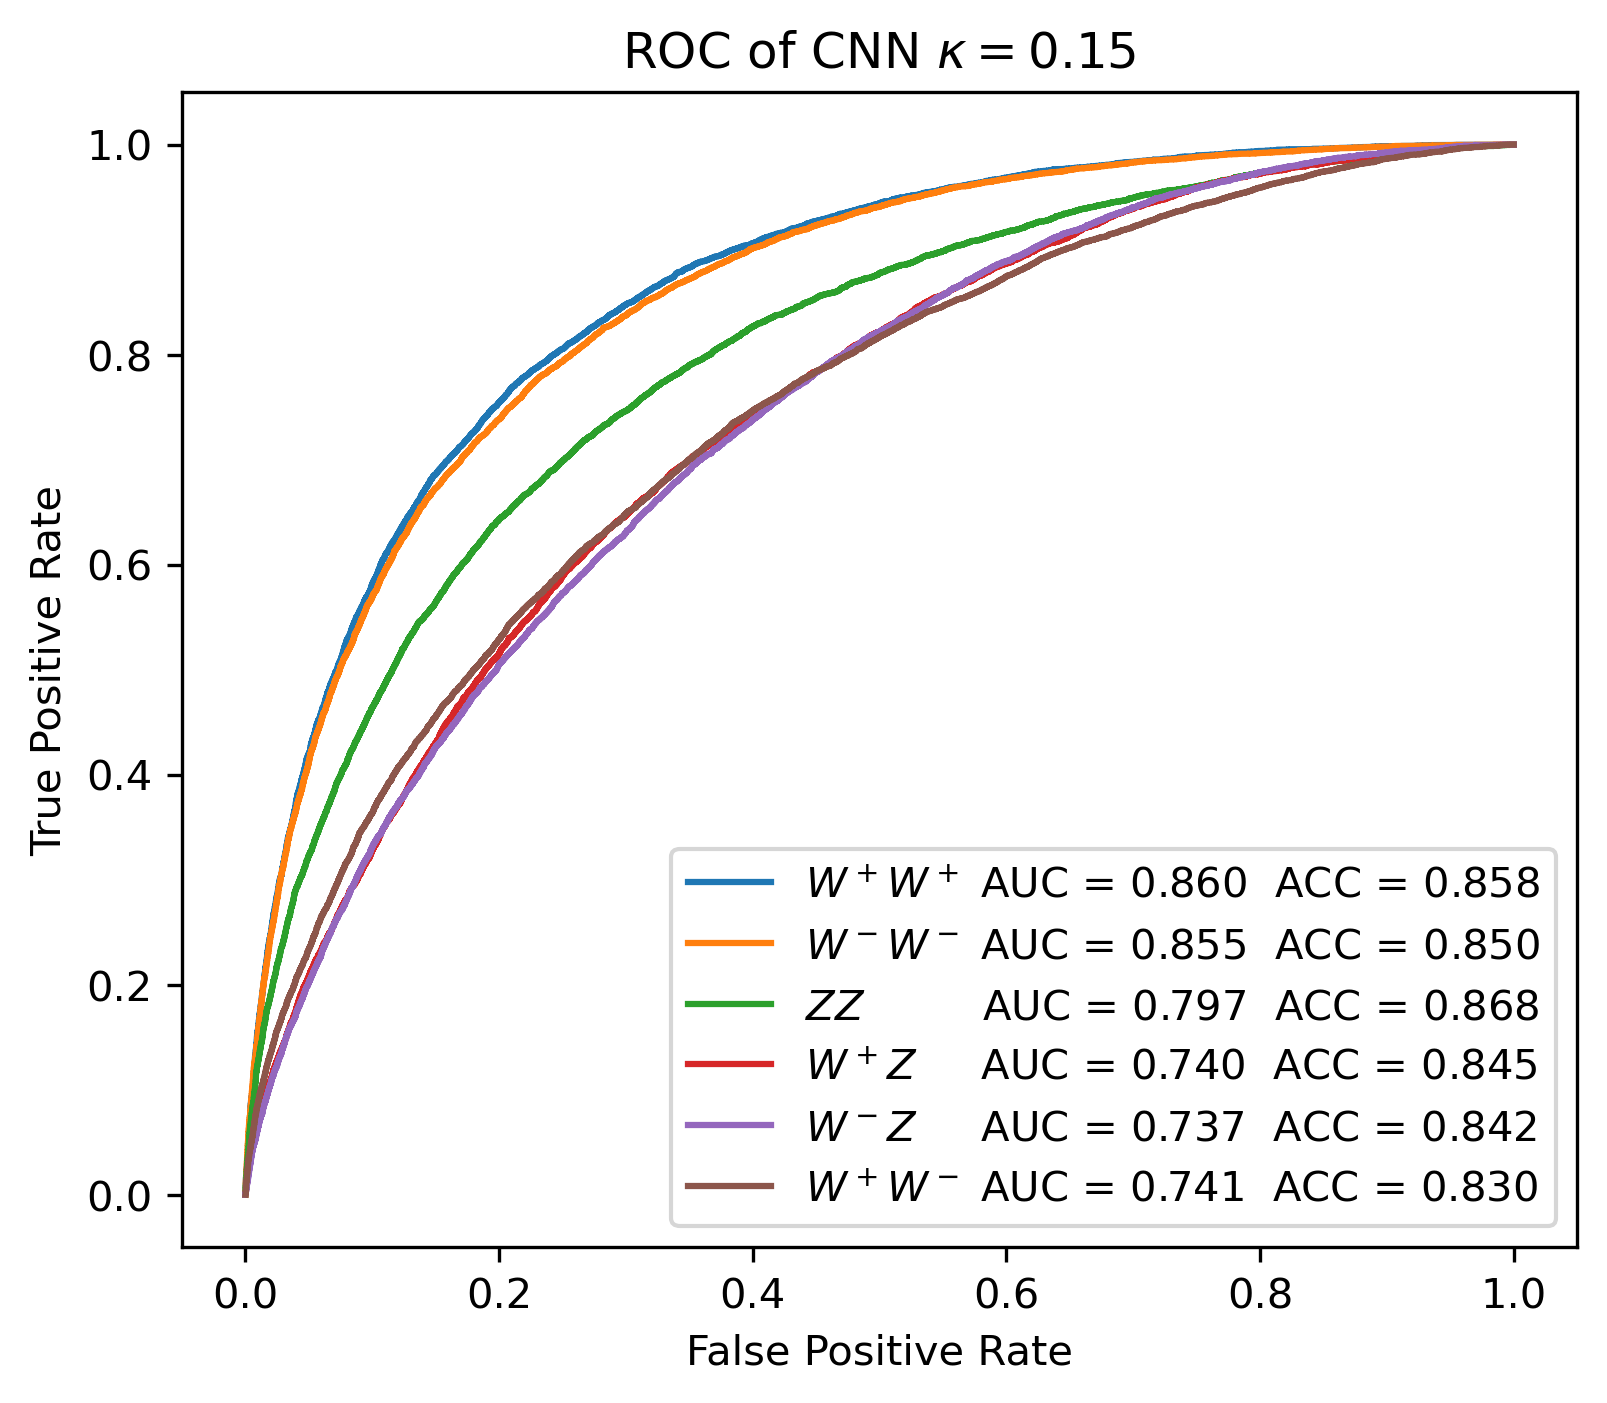
\includegraphics[width=0.65\textwidth]{event_ROC_CNN_kappa0.15-1000k.png}
			\caption{CNN's ROC of each event type. $\kappa=0.15$.}
			\label{fig:CNN_event_roc_015}
		\end{figure}
		\begin{figure}[htpb]
			\centering
			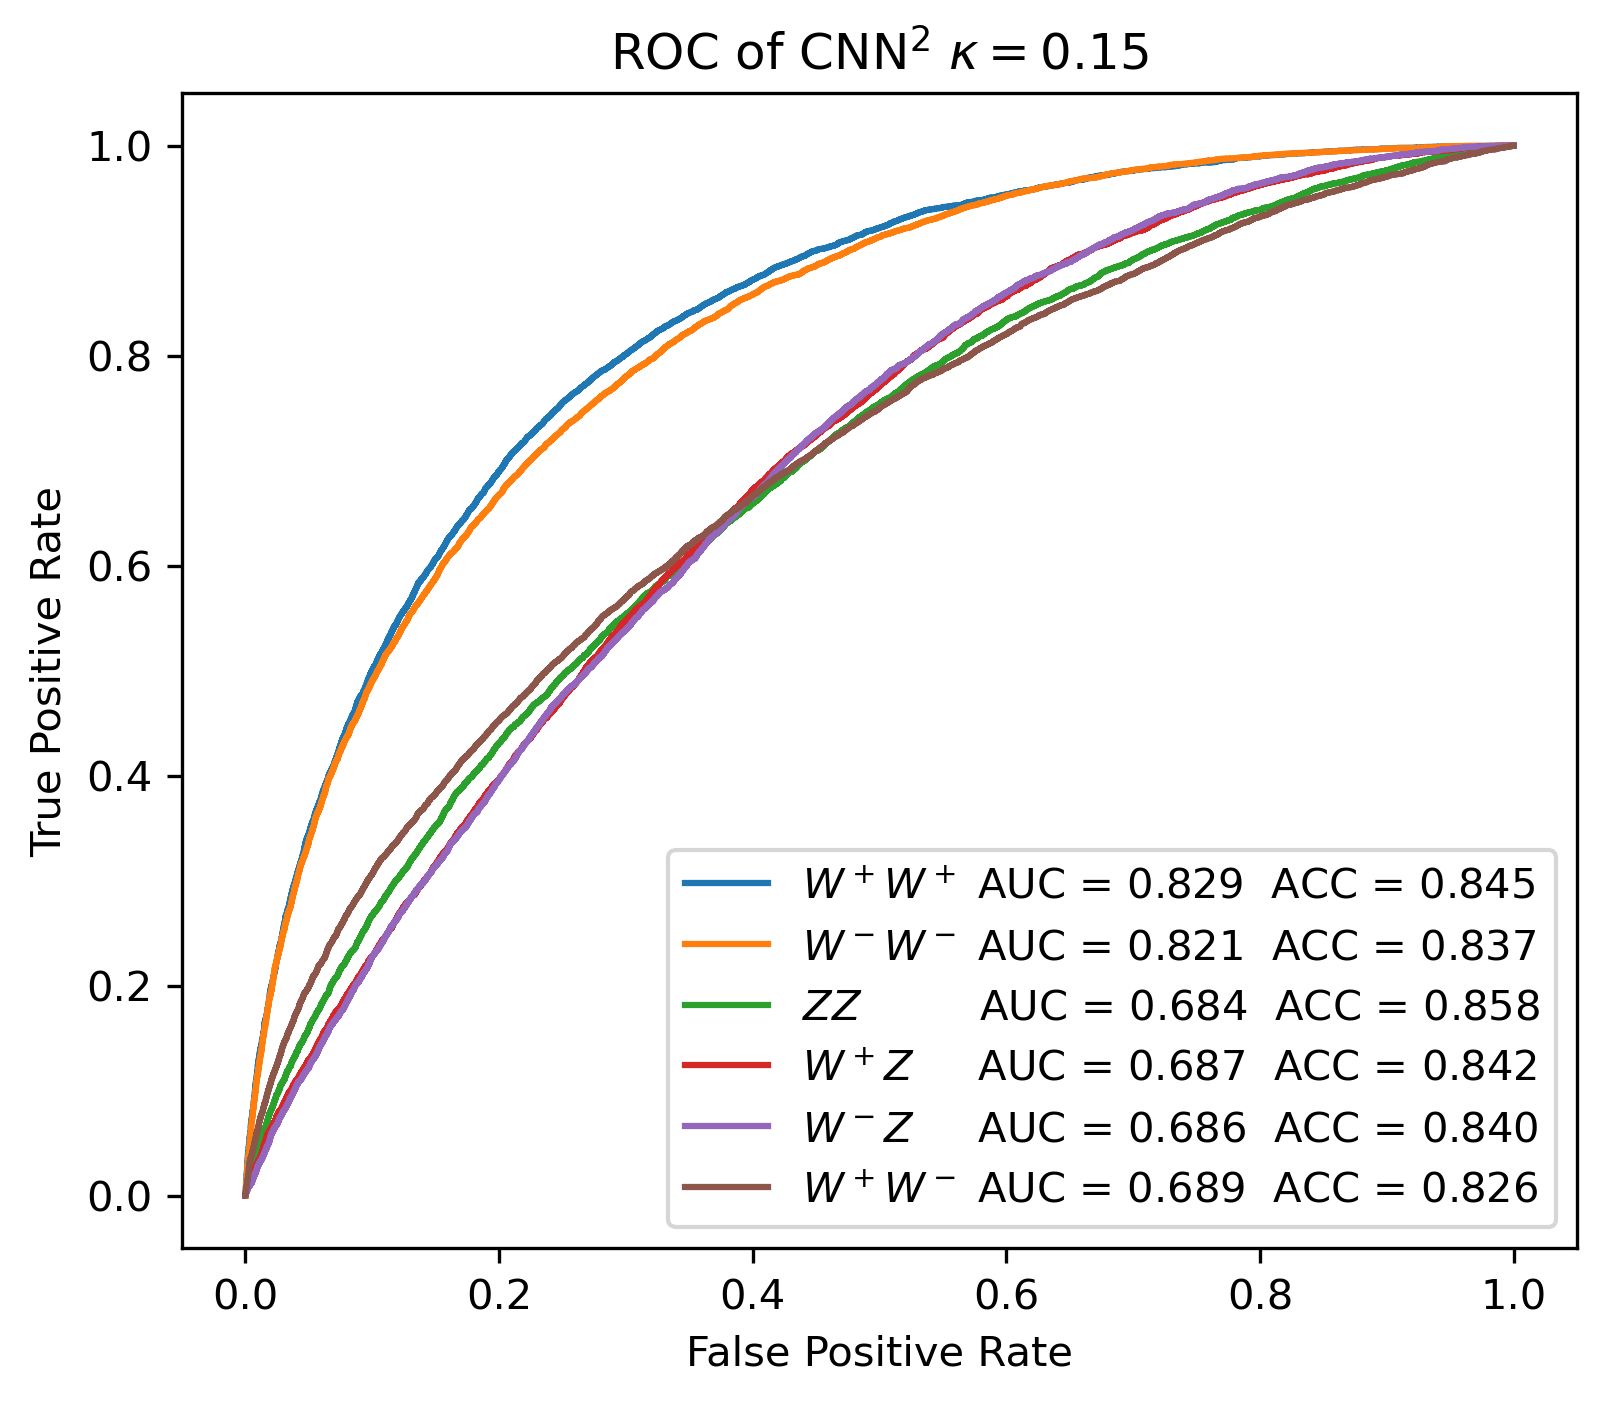
\includegraphics[width=0.65\textwidth]{event_ROC_CNNsq_kappa0.15-1000k.png}
			\caption{CNN$^2$'s ROC of each event type. $\kappa=0.15$.}
			\label{fig:CNNsq_event_roc_015}
		\end{figure}
	% subsection full_event_training_results (end)	
% section full_event_training (end)		
\section{Requirements of forward jet}% (fold)
\label{sec:requirements_of_forward_jet}
	In this section, the event selection criteria are modified. The $\Delta \eta$ and $p_\text{T}$ cuts on the forward jets were applied. The event image constructed method remained the same as the Sec. \ref{sub:full_event_sample_pre_processing}. 
	\subsection{Full event sample selection}% (fold)
	\label{sub:full_event_sample_selection_modified}
		The requirements of vector boson jet:
		\begin{enumerate}
			\item The transverse momentum of vector boson jets are required $p_\text{T} \in (350, 450) \text{ GeV}$ and in range $\abs{\eta}<1$.
			\item Merging: The angular distance between the two quarks decayed from the vector boson is required $\Delta R(q_1,q_2) < 0.6$.
			\item Matching: The vector boson and jet are matched if $\Delta R(V,j) < 0.1$.
		\end{enumerate}
		The events with less than two matching vector boson jets will be discarded.

		The forward jets are selected by the two highest $p_\text{T}$ jets from the remaining jets and need to satisfy the following requirements:
		\begin{enumerate}
			\item The transverse momentum of forward jets are required $p_\text{T} > \text{30 GeV}$.
			\item The difference of pseudorapidity of the two forward jets is required $\abs{\Delta \eta} > 2$.
		\end{enumerate}
		The event will be discarded if the forward jets can not pass the above requirements.
	% subsection full_event_sample_selection_modified (end)
	\subsection{Training results}% (fold)
	\label{sub:training_results}
		Select the samples again, where the forward jet cuts were applied. The event sample size for each type is presented in Table \ref{tab:full_event_sample_size_forward_jet_cut}
		\begin{table}[htpb]
			\centering
			\caption{The sample size for each type. 80\% samples are used in training, and 20\% samples are used in testing.}
			\label{tab:full_event_sample_size_forward_jet_cut}
			\begin{tabular}{c|c|c|c|c|c|c|c}
			Case & $\kappa$ & $W^+W^+$ & $W^-W^-$ & $ZZ$ & $W^+Z$ & $W^-Z$ & $W^+W^-$ \\ \hline
			1    & 0.15     & 36k      & 37k      & 29k  & 32k    & 33k    & 36k      
			\end{tabular}
		\end{table}

		The training results are summarized in Table \ref{tab:training_result_event_forward_jet_cut}. The training results are a little worse than Table \ref{tab:training_result_event}.
		\begin{table}[htpb]
			\centering
			\caption{The training results of the full event. The forward jet cuts were applied to the samples.}
			\label{tab:training_result_event_forward_jet_cut}
			\resizebox{\textwidth}{!}{
			\begin{tabular}{c|c|c|cc|cc|cc|cc|cc|cc}
										 &                    & Overall & \multicolumn{2}{c}{$W^+W^+$} & \multicolumn{2}{c}{$W^-W^-$} & \multicolumn{2}{c}{$ZZ$} & \multicolumn{2}{c}{$W^+Z$} & \multicolumn{2}{c}{$W^-Z$} & \multicolumn{2}{c}{$W^+W^-$} \\
					  & Sample             & ACC   & AUC   & ACC   & AUC   & ACC   & AUC   & ACC   & AUC   & ACC   & AUC   & ACC   & AUC   & ACC   \\ \hline
			CNN       & \multirow{2}{*}{1} & 0.440 & 0.858 & 0.858 & 0.849 & 0.849 & 0.791 & 0.868 & 0.731 & 0.845 & 0.729 & 0.837 & 0.736 & 0.827 \\
			CNN${}^2$ &                    & 0.374 & 0.831 & 0.846 & 0.818 & 0.837 & 0.679 & 0.858 & 0.684 & 0.844 & 0.683 & 0.836 & 0.690 & 0.824			
			\end{tabular}			
			}
		\end{table}

	% subsection training_results (end)	
% section requirements_of_forward_jet (end)	
\section{Change the resolution}% (fold)
\label{sec:change_the_resolution}
	This section changes the resolution of the event image. In the pixelating step, the $15 \times 15$ and $25 \times 25$ are used. 
	\subsection{Training results of different resolution}% (fold)
	\label{sub:training_results_of_different_resolution}
		The resolution in the pixelating step was changed to $15 \times 15$ and $25 \times 25$. Then use these samples to train the model. The training results are summarized in Table \ref{tab:training_result_event_resolution}. When the resolution decrease, the overall accuracy also decreases.

		The samples rescaled after pixelating are used in training to reduce the image size effect. For example, the image is pixelated with size $15 \times 15$, then rescale back to $75 \times 75$.  The training results are shown in Table \ref{tab:training_result_event_resolution_rescale}.
		\begin{table}[htpb]
			\centering
			\caption{The training results of the full event. The $N \times N$ means the resolution in the pixelating step.}
			\label{tab:training_result_event_resolution}
			\resizebox{\textwidth}{!}{
			\begin{tabular}{c|c|c|cc|cc|cc|cc|cc|cc}
										 &                    & Overall & \multicolumn{2}{c}{$W^+W^+$} & \multicolumn{2}{c}{$W^-W^-$} & \multicolumn{2}{c}{$ZZ$} & \multicolumn{2}{c}{$W^+Z$} & \multicolumn{2}{c}{$W^-Z$} & \multicolumn{2}{c}{$W^+W^-$} \\
			    & Sample         & ACC   & AUC   & ACC   & AUC   & ACC   & AUC   & ACC   & AUC   & ACC   & AUC   & ACC   & AUC   & ACC   \\ \hline
			CNN & $75 \times 75$ & 0.440 & 0.858 & 0.858 & 0.849 & 0.849 & 0.791 & 0.868 & 0.731 & 0.845 & 0.729 & 0.837 & 0.736 & 0.827 \\
			CNN & $25 \times 25$ & 0.378 & 0.830 & 0.845 & 0.820 & 0.838 & 0.692 & 0.856 & 0.685 & 0.841 & 0.687 & 0.836 & 0.690 & 0.827 \\
			CNN & $15 \times 15$ & 0.349 & 0.814 & 0.843 & 0.806 & 0.832 & 0.614 & 0.857 & 0.668 & 0.839 & 0.668 & 0.835 & 0.669 & 0.827			
			\end{tabular}			
			}
		\end{table}

		\begin{table}[htpb]
			\centering
			\caption{The training results of the full event. The samples are rescaled back to $75 \times  75$.}
			\label{tab:training_result_event_resolution_rescale}
			\resizebox{\textwidth}{!}{
			\begin{tabular}{c|c|c|cc|cc|cc|cc|cc|cc}
										 &                    & Overall & \multicolumn{2}{c}{$W^+W^+$} & \multicolumn{2}{c}{$W^-W^-$} & \multicolumn{2}{c}{$ZZ$} & \multicolumn{2}{c}{$W^+Z$} & \multicolumn{2}{c}{$W^-Z$} & \multicolumn{2}{c}{$W^+W^-$} \\
			    & Sample         & ACC   & AUC   & ACC   & AUC   & ACC   & AUC   & ACC   & AUC   & ACC   & AUC   & ACC   & AUC   & ACC   \\ \hline
			CNN & $75 \times 75$ & 0.440 & 0.858 & 0.858 & 0.849 & 0.849 & 0.791 & 0.868 & 0.731 & 0.845 & 0.729 & 0.837 & 0.736 & 0.827 \\
			CNN & $25 \times 25 \to 75 \times 75$ & 0.390 & 0.837 & 0.845 & 0.826 & 0.839 & 0.706 & 0.858 & 0.694 & 0.846 & 0.694 & 0.837 & 0.697 & 0.826 \\
			CNN & $15 \times 15 \to 75 \times 75$ & 0.362 & 0.823 & 0.843 & 0.812 & 0.833 & 0.654 & 0.854 & 0.676 & 0.844 & 0.674 & 0.838 & 0.677 & 0.828
			\end{tabular}			
			}
		\end{table}

		Compared to these two Tables, there is an improvement when the image size was rescaled back to $75 \times  75$.
	% subsection training_results_of_different_resolution (end)
% section change_the_resolution (end)		
\section{Middle layer output}% (fold)
\label{sec:middle_layer_output}
	In this section, the middle layer outputs of the event image are printed out. The different resolution samples are used and the rescaled samples are also used. The same CNN structure is used for training.

	The results are summarized in Figure \ref{fig:CNN_middle_layer_output}. 
	\begin{figure}[htpb]
		\centering
		\subfloat[$75\times 75$]{
			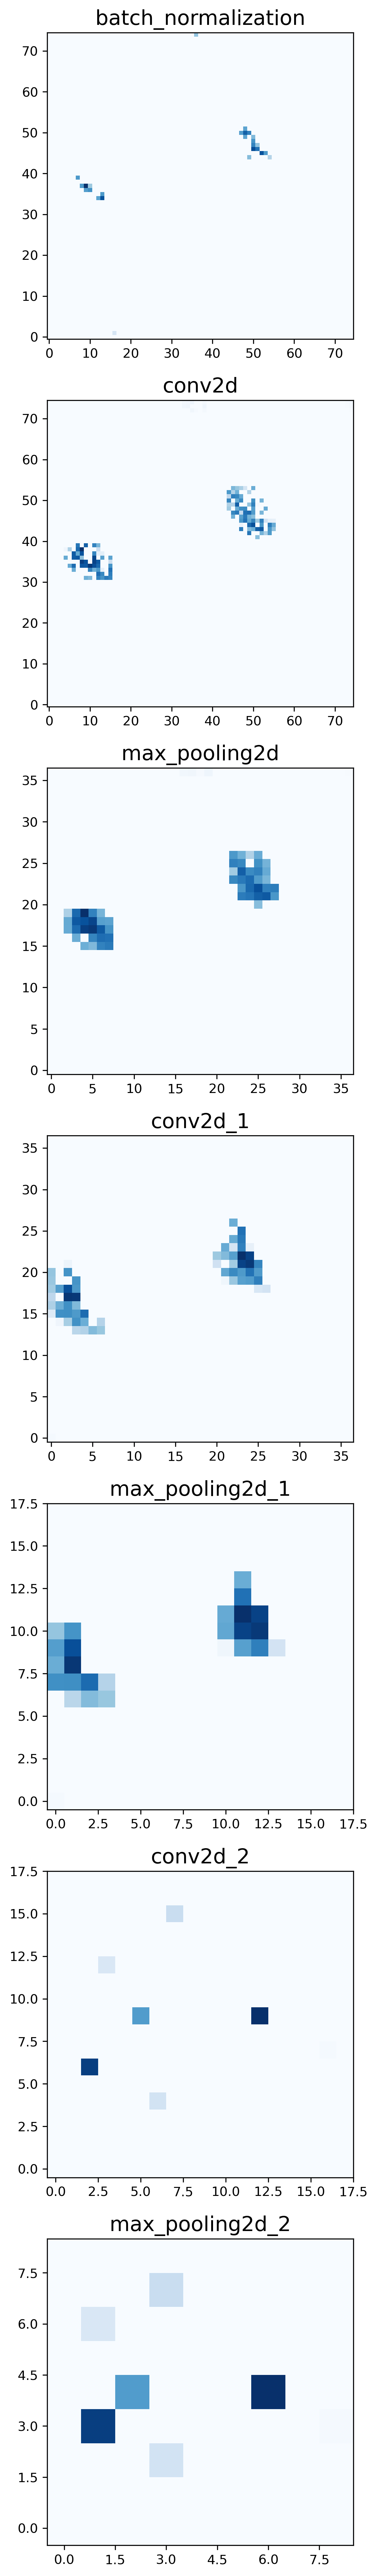
\includegraphics[width=0.17\textwidth]{CNN_middle_layer_output_75x75.png}
		}
		\subfloat[$25\times 25$]{
			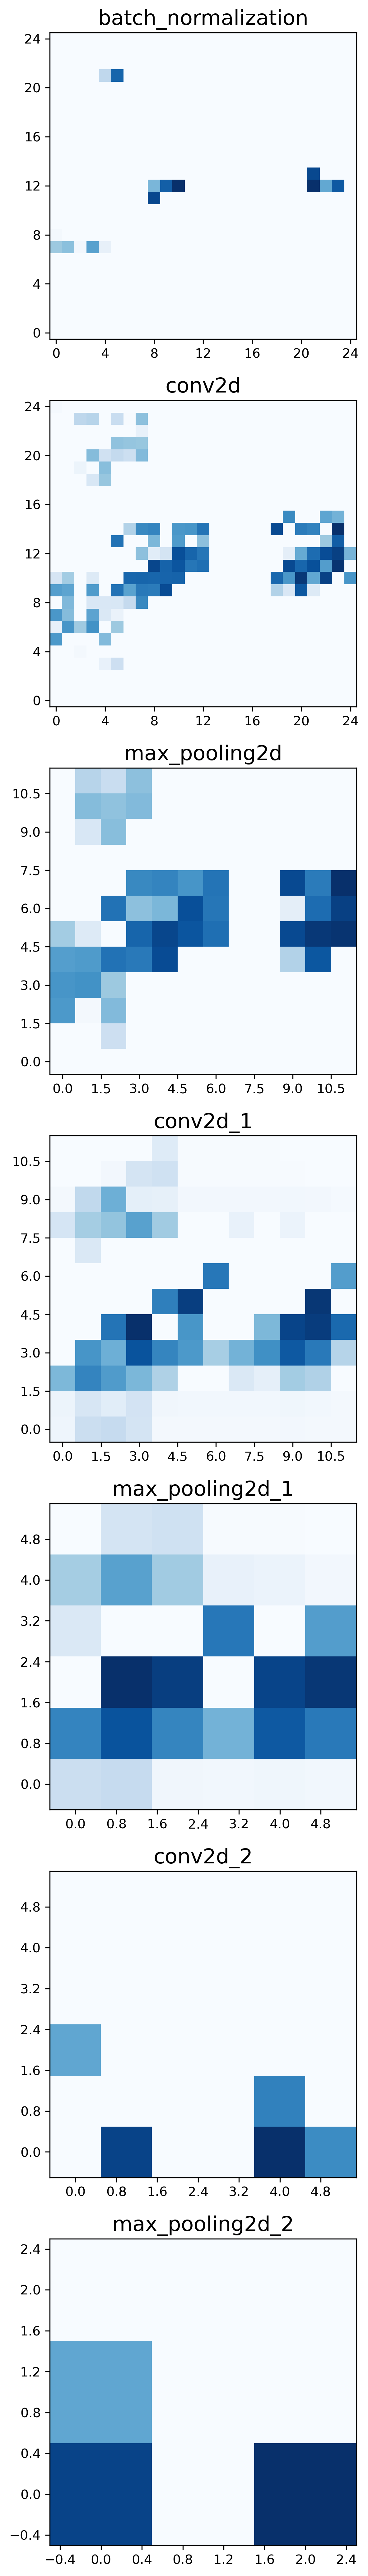
\includegraphics[width=0.17\textwidth]{CNN_middle_layer_output_25x25.png}
		}
		\subfloat[$25 \times 25 \to 75 \times 75$]{
			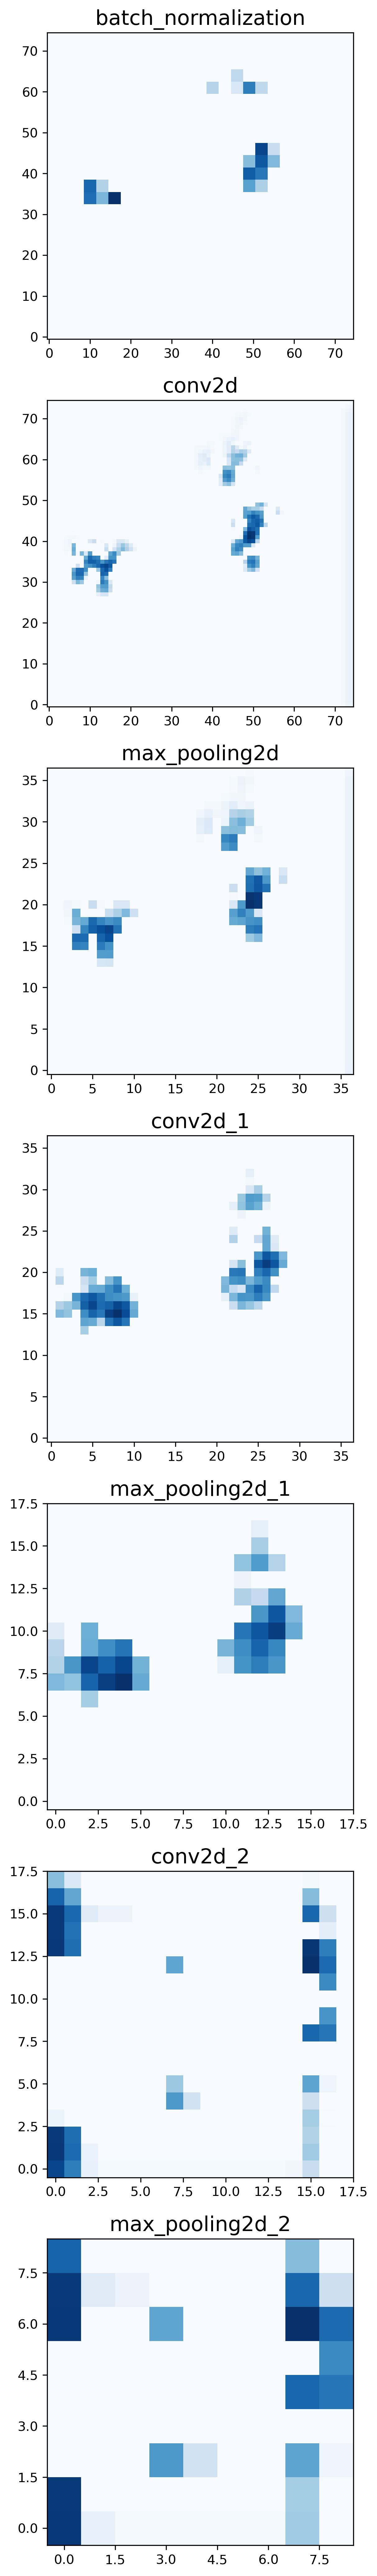
\includegraphics[width=0.17\textwidth]{CNN_middle_layer_output_25x25-75x75.png}
		}
		\subfloat[$15 \times 15$]{
			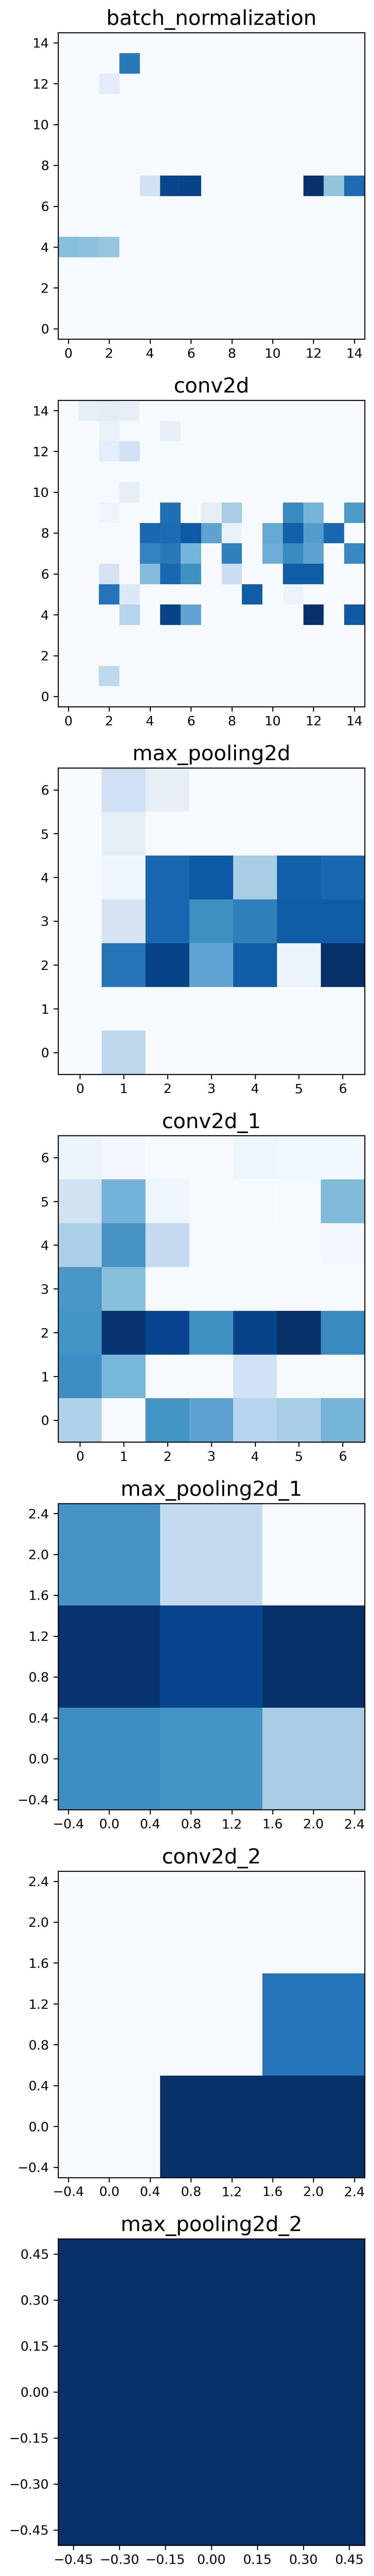
\includegraphics[width=0.17\textwidth]{CNN_middle_layer_output_15x15.png}
		}
		\subfloat[$15 \times 15 \to 75 \times 75$]{
			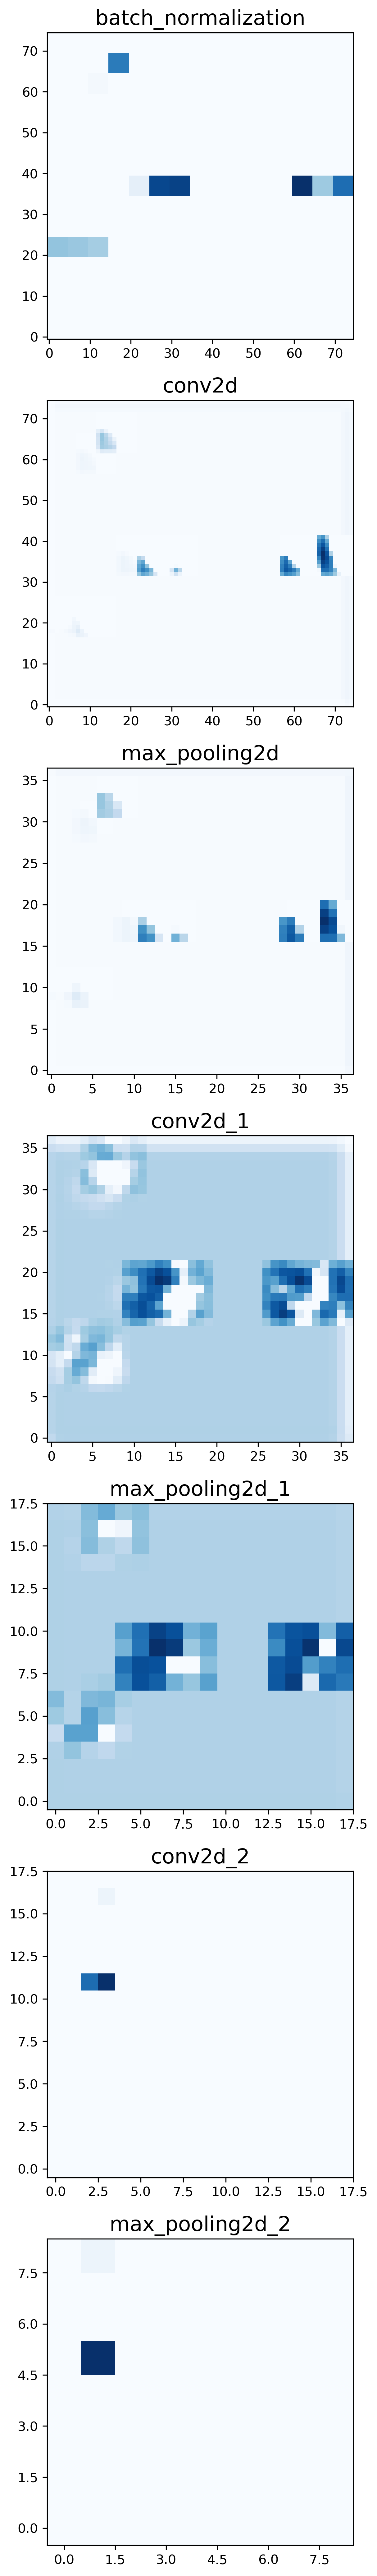
\includegraphics[width=0.17\textwidth]{CNN_middle_layer_output_15x15-75x75.png}
		}
		\caption{The middle layer output of event image. The resolution $75\times 75$, $25\times 25$, and $15\times 15$ are used. The rescaled ones are also shown for resolution $25\times 25$ and $15\times 15$.}
		\label{fig:CNN_middle_layer_output}
	\end{figure}
% section middle_layer_output (end)		
\end{document} 
